% ******************************* PhD Thesis Template **************************
% Please have a look at the README.md file for info on how to use the template

\documentclass[a4paper,12pt,times,authoryear,print,index]{PhDThesisPSnPDF}

\setlength{\parskip}{6pt}%
% \setlength{\parindent}{0pt}%

% ******************************************************************************
% ******************************* Class Options ********************************
% *********************** See README for more details **************************
% ******************************************************************************

% `a4paper'(The University of Cambridge PhD thesis guidelines recommends a page
% size a4 - default option) or `a5paper': A5 Paper size is also allowed as per
% the Cambridge University Engineering Deparment guidelines for PhD thesis
%
% `11pt' or `12pt'(default): Font Size 10pt is NOT recommended by the University
% guidelines
%
% `oneside' or `twoside'(default): Printing double side (twoside) or single
% side.
%
% `print': Use `print' for print version with appropriate margins and page
% layout. Leaving the options field blank will activate Online version.
%
% `index': For index at the end of the thesis
%
% `draftclassic': For draft mode without loading any images (same as draft in book)
%
% `draft': Special draft mode with line numbers, images, and water mark with
% timestamp and custom text. Position of the text can also be modified.
%
% `abstract': To generate only the title page and abstract page with
% dissertation title and name, to submit to the Student Registry
%
% `chapter`: This option enables only the specified chapter and it's references
%  Useful for review and corrections.
%
% ************************* Custom Page Margins ********************************
%
% `custommargin`: Use `custommargin' in options to activate custom page margins,
% which can be defined in the preamble.tex. Custom margin will override
% print/online margin setup.
%
% *********************** Choosing the Fonts in Class Options ******************
%
% `times' : Times font with math support. (The Cambridge University guidelines
% recommend using times)
%
% `fourier': Utopia Font with Fourier Math font (Font has to be installed)
%            It's a free font.
%
% `customfont': Use `customfont' option in the document class and load the
% package in the preamble.tex
%
% default or leave empty: `Latin Modern' font will be loaded.
%
% ********************** Choosing the Bibliography style ***********************
%
% `authoryear': For author-year citation eg., Krishna (2013)
%
% `numbered': (Default Option) For numbered and sorted citation e.g., [1,5,2]
%
% `custombib': Define your own bibliography style in the `preamble.tex' file.
%              `\RequirePackage[square, sort, numbers, authoryear]{natbib}'.
%              This can be also used to load biblatex instead of natbib
%              (See Preamble)
%
% **************************** Choosing the Page Style *************************
%
% `default (leave empty)': For Page Numbers in Header (Left Even, Right Odd) and
% Chapter Name in Header (Right Even) and Section Name (Left Odd). Blank Footer.
%
% `PageStyleI': Chapter Name next & Page Number on Even Side (Left Even).
% Section Name & Page Number in Header on Odd Side (Right Odd). Footer is empty.
%
% `PageStyleII': Chapter Name on Even Side (Left Even) in Header. Section Number
% and Section Name in Header on Odd Side (Right Odd). Page numbering in footer

% Uncomment to change page style
%\pagestyle{PageStyleII}

% ********************************** Preamble **********************************
% Preamble: Contains packages and user-defined commands and settings
% ******************************************************************************
% ****************************** Custom Margin *********************************

% Add `custommargin' in the document class options to use this section
% Set {innerside margin / outerside margin / topmargin / bottom margin}  and
% other page dimensions
\ifsetCustomMargin
  \RequirePackage[left=37mm,right=30mm,top=35mm,bottom=30mm]{geometry}
  \setFancyHdr % To apply fancy header after geometry package is loaded
\fi

% Add spaces between paragraphs
%\setlength{\parskip}{0.5em}
% Ragged bottom avoids extra whitespaces between paragraphs
\raggedbottom
% To remove the excess top spacing for enumeration, list and description
%\usepackage{enumitem}
%\setlist[enumerate,itemize,description]{topsep=0em}

% *****************************************************************************
% ******************* Fonts (like different typewriter fonts etc.)*************

% Add `customfont' in the document class option to use this section

\ifsetCustomFont
  % Set your custom font here and use `customfont' in options. Leave empty to
  % load computer modern font (default LaTeX font).
  %\RequirePackage{helvet}

  % For use with XeLaTeX
  %  \setmainfont[
  %    Path              = ./libertine/opentype/,
  %    Extension         = .otf,
  %    UprightFont = LinLibertine_R,
  %    BoldFont = LinLibertine_RZ, % Linux Libertine O Regular Semibold
  %    ItalicFont = LinLibertine_RI,
  %    BoldItalicFont = LinLibertine_RZI, % Linux Libertine O Regular Semibold Italic
  %  ]
  %  {libertine}
  %  % load font from system font
  %  \newfontfamily\libertinesystemfont{Linux Libertine O}
\fi

% *****************************************************************************
% **************************** Custom Packages ********************************

% ************************* Algorithms and Pseudocode **************************

%\usepackage{algpseudocode}


% ********************Captions and Hyperreferencing / URL **********************

% Captions: This makes captions of figures use a boldfaced small font.
%\RequirePackage[small,bf]{caption}

\RequirePackage[labelsep=space,tableposition=top]{caption}
\renewcommand{\figurename}{Fig.} %to support older versions of captions.sty


% *************************** Graphics and figures *****************************

%\usepackage{rotating}
%\usepackage{wrapfig}

% Uncomment the following two lines to force Latex to place the figure.
% Use [H] when including graphics. Note 'H' instead of 'h'
%\usepackage{float}
%\restylefloat{figure}

% Subcaption package is also available in the sty folder you can use that by
% uncommenting the following line
% This is for people stuck with older versions of texlive
%\usepackage{sty/caption/subcaption}
\usepackage{subcaption}

% ********************************** Tables ************************************
\usepackage{booktabs} % For professional looking tables
\usepackage{multirow}
\usepackage{amsmath}
%\usepackage{multicol}
%\usepackage{longtable}
%\usepackage{tabularx}

\usepackage{bm}
%bold Greek letters
\usepackage{pdfrender}
\newcommand*{\boldgreek}[1]{%
  \textpdfrender{%
    TextRenderingMode=FillStroke,%
    LineWidth=.35pt,%
  }{#1}%
}
%algorithms
\usepackage{algorithm}
\usepackage[noend]{algpseudocode}

%theorems
\newtheorem{theorem}{Theorem}[section]

%dates
\usepackage{datetime}
\newdate{date}{12}{08}{2019}
\date{\displaydate{date}}
% circle with numbers
\usepackage{IEEEtrantools,stackengine}
\stackMath
\usepackage{tikz}
\newcommand\encircle[1]{%
  \tikz[baseline=(X.base)] 
    \node (X) [draw, shape=circle, inner sep=0] {\strut #1};}
% *********************************** SI Units *********************************
\usepackage{siunitx} % use this package module for SI units
\usepackage{wrapfig}

% ******************************* Line Spacing *********************************

% Choose linespacing as appropriate. Default is one-half line spacing as per the
% University guidelines

% \doublespacing
% \onehalfspacing
% \singlespacing


% ************************ Formatting / Footnote *******************************

% Don't break enumeration (etc.) across pages in an ugly manner (default 10000)
%\clubpenalty=500
%\widowpenalty=500

%\usepackage[perpage]{footmisc} %Range of footnote options


% *****************************************************************************
% *************************** Bibliography  and References ********************

%\usepackage{cleveref} %Referencing without need to explicitly state fig /table

% Add `custombib' in the document class option to use this section
\ifuseCustomBib
   \RequirePackage[square, sort, numbers, authoryear]{natbib} % CustomBib

% If you would like to use biblatex for your reference management, as opposed to the default `natbibpackage` pass the option `custombib` in the document class. Comment out the previous line to make sure you don't load the natbib package. Uncomment the following lines and specify the location of references.bib file

% \RequirePackage[backend=biber, style=numeric-comp, citestyle=numeric, sorting=nty, natbib=true]{biblatex}
% \addbibresource{References/references} %Location of references.bib only for biblatex, Do not omit the .bib extension from the filename.

\fi

% changes the default name `Bibliography` -> `References'
\renewcommand{\bibname}{References}


% ******************************************************************************
% ************************* User Defined Commands ******************************
% ******************************************************************************

% *********** To change the name of Table of Contents / LOF and LOT ************

%\renewcommand{\contentsname}{My Table of Contents}
%\renewcommand{\listfigurename}{My List of Figures}
%\renewcommand{\listtablename}{My List of Tables}


% ********************** TOC depth and numbering depth *************************

\setcounter{secnumdepth}{2}
\setcounter{tocdepth}{2}


% ******************************* Nomenclature *********************************

% To change the name of the Nomenclature section, uncomment the following line

%\renewcommand{\nomname}{Symbols}


% ********************************* Appendix ***********************************

% The default value of both \appendixtocname and \appendixpagename is `Appendices'. These names can all be changed via:

%\renewcommand{\appendixtocname}{List of appendices}
%\renewcommand{\appendixname}{Appndx}

% *********************** Configure Draft Mode **********************************

% Uncomment to disable figures in `draft'
%\setkeys{Gin}{draft=true}  % set draft to false to enable figures in `draft'

% These options are active only during the draft mode
% Default text is "Draft"
%\SetDraftText{DRAFT}

% Default Watermark location is top. Location (top/bottom)
%\SetDraftWMPosition{bottom}

% Draft Version - default is v1.0
%\SetDraftVersion{v1.1}

% Draft Text grayscale value (should be between 0-black and 1-white)
% Default value is 0.75
%\SetDraftGrayScale{0.8}


% ******************************** Todo Notes **********************************
%% Uncomment the following lines to have todonotes.

%\ifsetDraft
%	\usepackage[colorinlistoftodos]{todonotes}
%	\newcommand{\mynote}[1]{\todo[author=kks32,size=\small,inline,color=green!40]{#1}}
%\else
%	\newcommand{\mynote}[1]{}
%	\newcommand{\listoftodos}{}
%\fi

% Example todo: \mynote{Hey! I have a note}

% ******************************** Highlighting Changes **********************************
%% Uncomment the following lines to be able to highlight text/modifications.
%\ifsetDraft
%  \usepackage{color, soul}
%  \newcommand{\hlc}[2][yellow]{{\sethlcolor{#1} \hl{#2}}}
%  \newcommand{\hlfix}[2]{\texthl{#1}\todo{#2}}
%\else
%  \newcommand{\hlc}[2]{}
%  \newcommand{\hlfix}[2]{}
%\fi

% Example highlight 1: \hlc{Text to be highlighted}
% Example highlight 2: \hlc[green]{Text to be highlighted in green colour}
% Example highlight 3: \hlfix{Original Text}{Fixed Text}

% *****************************************************************************
% ******************* Better enumeration my MB*************
\usepackage{enumitem}


% ************************ Thesis Information & Meta-data **********************
% Thesis title and author information, refernce file for biblatex
% ************************ Thesis Information & Meta-data **********************
%% The title of the thesis
\title{Disentangling Sources of Uncertainty for Active Exploration}

% \subtitle{Using the CUED template}

%% The full name of the author
\author{David Lines}

%% Department (eg. Department of Engineering, Maths, Physics)
\dept{Department of Engineering}

%% University and Crest
\university{University of Cambridge}
% Crest minimum should be 30mm.
\crest{
\includegraphics[width=0.2\textwidth]{Figs/UniversityShield/University_Crest.pdf}}
%% Use this crest, if you are using the college crest
%% Crest long miminum should be 65mm
%\crest{
\includegraphics[width=0.45\textwidth]{University_Crest_Long}}

%% College shield [optional] 
% Crest minimum should be 30mm.
\collegeshield{
\includegraphics[width=0.25\textwidth]{Figs/CollegeShield/magdalene-crest.jpg}}


%% Supervisor (optional)
%% for multiple supervisors, append each supervisor with the \newline command
\supervisor{Prof. C.E. Rasmussen\newline
Dr M. Van Der Wilk}

%% Supervisor Role (optional) - Supervisor (default) or advisor
% \supervisorrole{\textbf{Supervisors: }}
%% if no title is desired:
% \supervisorrole{}

%% Supervisor line width: required to align supervisors
%\supervisorlinewidth{0.35\textwidth}

%% Advisor (optional)
%% for multiple advisors, append each advisor with the \newline command
%\advisor{Dr. A. Advisor\newline
%Dr. B. Advisor}
     
%% Advisor Role (optional) - Advisor (default) or leave empty
% \advisorrole{Advisors: }
%% if no title is required
% \advisorrole{}

%% Advisor line width: required to align supervisors
%\advisorlinewidth{0.25\textwidth}


%% You can redefine the submission text:
% Default as per the University guidelines:
% ``This dissertation is submitted for the degree of''
%\renewcommand{\submissiontext}{change the default text here if needed}

%% Full title of the Degree
\degreetitle{Master of Philosophy}

%% College affiliation (optional)
\college{Magdalene College}

%% Submission date
% Default is set as {\monthname[\the\month]\space\the\year}
%\degreedate{September 2014} 

%% Meta information
\subject{LaTeX} \keywords{{LaTeX} {PhD Thesis} {Engineering} {University of
Cambridge}}


% ***************************** Abstract Separate ******************************
% To printout only the titlepage and the abstract with the PhD title and the
% author name for submission to the Student Registry, use the `abstract' option in
% the document class.

\ifdefineAbstract
 \pagestyle{empty}
 \includeonly{Declaration/declaration, Abstract/abstract}
\fi

% ***************************** Chapter Mode ***********************************
% The chapter mode allows user to only print particular chapters with references
% Title, Contents, Frontmatter are disabled by default
% Useful option to review a particular chapter or to send it to supervisior.
% To use choose `chapter' option in the document class

\ifdefineChapter
 \includeonly{Chapter3/chapter3}
\fi

% ******************************** Front Matter ********************************
\begin{document}

\frontmatter

\maketitle

% ******************************* Thesis Declaration ***************************

\begin{declaration}

I, David Lines of Magdalene College, being a candidate for the MPhil in Machine Learning and Machine Intelligence, hereby declare that this report and the work described in it are my own work, unaided except as may be specified below, and that the report does not contain material that has already been used to any substantial extent for a comparable purpose.
\\[0.5in]
This report makes use of the following software to aid in the production of the results:
\begin{enumerate}
   \item SSGP code: Available at: \url{http://www.tsc.uc3m.es/~miguel/simpletutorialssgp.php}
   \begin{itemize}
     \item Code modified to include sampling from the posterior distribution. 
     \item Used in the production of results in Section \ref{S:results}.
   \end{itemize}
   \item PILCO MATLAB code: Available at: \url{http://mlg.eng.cam.ac.uk/pilco/}
   \begin{itemize}
     \item Code modified to include the Monte-Carlo uncertainty decomposition method presented in Section \ref{S:monte-carlo-estimate} and the SSGP code listed above.
     \item Used in the production of results in Section \ref{S:results}.
   \end{itemize}
\end{enumerate}
% \\[1in]
.
% Author and date will be inserted automatically from thesis.tex \author \degreedate
\end{declaration}


% ************************** Thesis Abstract *****************************
% Use `abstract' as an option in the document class to print only the titlepage and the abstract.
\begin{abstract}
PILCO evaluates and minimises the expected cost by cascading uncertain inputs through the GP dynamics model. This approach only allows PILCO to make decisions based on the total uncertainty on the cost. I use variance as a metric for uncertainty and employ the law of total variance to decompose the total cost uncertainty into its aleatoric and epistemic components. I introduce a gold-standard Monte-Carlo scheme to separately estimate each quantity by propagating trajectories through an approximation to PILCO’s dynamics model. Finally, I show that when PILCO is learning efficiently it is selecting policies associated with a high ratio of epistemic cost uncertainty to total cost uncertainty.
\end{abstract}

% ************************** Thesis Acknowledgements **************************

\begin{acknowledgements}      
I would like to acknowledge my supervisors Professor C.E. Rasmussen and Dr M. Van Der Wilk 
for providing excellent advice and guidance throughout the course of the project.
\end{acknowledgements}



% *********************** Adding TOC and List of Figures ***********************

\tableofcontents

\listoffigures

% \listoftables
\listofalgorithms

% \printnomenclature[space] space can be set as 2em between symbol and description
%\printnomenclature[3em]

% \printnomenclature

% ******************************** Main Matter *********************************
\mainmatter

%!TEX root = ../thesis.tex
%*******************************************************************************
%*********************************** First Chapter *****************************
%*******************************************************************************

\chapter{Introduction}  %Title of the First Chapter

\ifpdf
    \graphicspath{{Chapter1/Figs/Raster/}{Chapter1/Figs/PDF/}{Chapter1/Figs/}}
\else
    \graphicspath{{Chapter1/Figs/Vector/}{Chapter1/Figs/}{Chapter1/Figures/}}
\fi


%********************************** %First Section  **************************************
\textit{Probabilistic Inference for Learning Control} or PILCO \citep{deisenroth2011pilco} is a model-based indirect policy search method for continuous state and action dynamical systems. PILCO evaluates a particular \textit{policy} by assuming that the distribution over inputs is Gaussian and propagating that distribution through its probabilistic representation of the transition dynamics under a particular policy. In doing so, it gains insight into the variety of states that could be visited under that policy and is able to make inferences about how effective the policy is at achieving low cost. However, this approach only allows PILCO to make decisions based on the total uncertainty as quantified by the models predictive distribution, when in fact there are two sources of uncertainty present in the system: \textit{aleatoric} and \textit{epistemic}. Aleatoric uncertainty is uncertainty due to unknowns that differ each time an agent encounters the environment (such as measurement noise) and is irreducible. Epistemic uncertainty arises from information that the agent could know in principle but currently does not, and can be reduced by observing more data. In model-based reinforcement learning, epistemic uncertainty is due to uncertainty about the model parameters. This means that in some situations PILCO could be exploring regions in the state space that are irrelevant for the task of learning control because it is making decisions based on the total uncertainty without knowledge of its constituents. In this case it could be targeting areas of high aleatoric uncertainty which could prohibit learning. 

In this dissertation I investigate how PILCO uses uncertainty in its decision making process. In particular, I disentangle and quantify the different sources of uncertainty in the model of the transition function under a given policy. PILCO is a direct policy search method and is formulated so that the \textit{cost function} is consulted directly; therefore, I examine the influence of the transition function uncertainty on cost uncertainty. I use variance as a metric for uncertainty and employ the law of total variance to decompose the total cost uncertainty into its constituents. I introduce a gold-standard Monte-Carlo scheme to separately estimate the aleatoric and epistemic uncertainties in the cost by propagating trajectories through an approximation to PILCO's dynamics model. Finally, I show that when PILCO is learning efficiently it is selecting policies associated with a high ratio of epistemic cost uncertainty to total cost uncertainty.

The aim of this dissertation is to lay the foundations for an active-exploration scheme to complement PILCO. In this dissertation I make the following contributions:
\begin{itemize}
    \item Present a variance decomposition that disentangles the sources of uncertainty in the model's predictive distribution that influence PILCO's cost under a particular policy $\pi$.
    \item Create a gold-standard Monte Carlo scheme that separates the two sources of uncertainty and quantifies them.
    \item Show that for complex environments PILCO's policy gradient method can get temporarily stuck in areas of low cost and low epistemic uncertainty and that this slows down learning.
    \item Show that when PILCO is learning efficiently, it is selecting policies that correspond to low cost and high epistemic uncertainty. 
\end{itemize}

\section{Background} %Section - 1.1 
\label{S:background}
\textit{Reinforcement learning} is a general sequential decision making framework that is best described as learning a mapping from situations to actions in an attempt to maximise a numerical reward signal. The agent, or learner, is not told what to do and so must embark on a mission of trial-and-error to discover actions that produce the most reward. In many cases, the action taken not only influences the instantaneous reward but also the next situation or state, and therefore, all future rewards as a consequence. To find a set of optimal actions given a sequence of situations, the agent must then take into account the effect of an action on all future rewards. These two ideas; trial-and-error search and delayed reward, are the two most distinguishing features of reinforcement learning \citep{sutton2018reinforcement}.

Another highly influential idea is the trade-off between \textit{exploration} and \textit{exploitation}. For an agent to maximise the long-term reward it must favour actions which it has previously tried and found to be successful in yielding high reward. However, in order to discover those actions, it must first have tried actions that it had not previously selected. The agent must \textit{exploit} its current knowledge of the system to gain a high reward but also \textit{explore} new strategies to improve its \textit{policy}. A dilemma arises in that exclusively executing either approach will lead to a failed task. The agent must interchangeably try both approaches and progressively tend towards actions that prove to be better at attaining high reward.

There are two main approaches to reinforcement learning; \textit{model-based} and \textit{model-free} methods. Model-free methods are explicit trial-and-error learners and directly use the experience they gain through interactions with an environment to make decisions. In contrast, model-based techniques use experience indirectly by building a model of the state transition dynamics and reward structure of the environment, and evaluate actions by searching this model \citep{glascher2010states}. Model-free methods are therefore said to rely on \textit{learning} whilst model-based methods primarily  rely on \textit{planning} \citep{sutton2018reinforcement}. 

Recently, model-free methods have achieved impressive performance in a range of complex tasks such as playing Atari games, receiving only pixels and game scores as inputs \citep{mnih2015human}. These methods, however, typically require millions of interactions with the environment before they achieve reasonable performance levels. The large number of required interactions can prohibit the use of these algorithms in some domains; such as mechanical systems with components that quickly wear out \citep{deisenroth2011pilco} or safety-critical systems where carrying out many field trials is prohibitively expensive. With computational power increasing exponentially, the primary bottleneck in the deployment of real-world reinforcement learning applications is fast becoming the number of interactions with the environment \citep{Wan2018ModelbasedRL}.

Model-based methods use field trials to create a belief about the underlying environment. There are several advantages to this approach, amongst others; the learning process can be more sample-efficient \citep{deisenroth2013gaussian}, prior knowledge and experience can be integrated more easily (particularly when Bayesian models are used) \citep{lopes2012exploration}, and more recently the incorporation of \textit{counterfactual} reasoning (making inferences about actions that were not actually taken) which can be complex to implement without an explicit model-based representation of the environment \citep{buesing2018woulda}. Model-based methods are, however, not without their challenges, building accurate representations of complex real-world environments is difficult and failing to do so can lead to highly suboptimal algorithm behaviour.

Until recently, model-based techniques had not been widely applied to real-world systems. One of the main reasons for this is they can suffer from model bias. This happens when, given a data set of observed state transitions, the learned model incorrectly assumes that it fully describes the environment, when in fact there are many plausible functions that could have generated the data (\cite{atkeson1997comparison}; \cite{schneider1997exploiting}). This is demonstrated in Fig \ref{Fig:model-bias} where a small data set of transitions are observed (left panel) and several transition functions exist that could have generated the data (centre panel). Selecting any single transition function can have severe consequences because predictions are then arbitrary at positions away from the data, but are claimed with full confidence \citep{deisenroth2011pilco}. 

PILCO \citep{deisenroth2011pilco} is a model-based indirect policy search method for continuous state and action dynamical systems. PILCO learns a probabilistic Bayesian representation of the dynamical systems it seeks to govern. Bayesian models explicitly quantify their uncertainty, and PILCO uses this information in a principled way to reduce model bias by explicitly incorporating model uncertainty into long-term planning. Fig \ref{Fig:model-bias} (right panel) shows how PILCO represents the observed data by placing a posterior distribution over the transition function. 

PILCO reports unprecedented data-efficiency for a variety of control tasks, such as the cart-pole and cart-double-pole problems. Surprisingly, it does so without any intentional exploration i.e. it is \textit{greedy}. Any exploration that does occur comes from one of three sources: first, the presence of stochasticity in the system; second, the use of a saturating cost function resulting in the controller favouring uncertain states \citep{deisenroth2013gaussian}; third, future controllers being informed of the performance of past controllers. 

\begin{figure}
\centering    
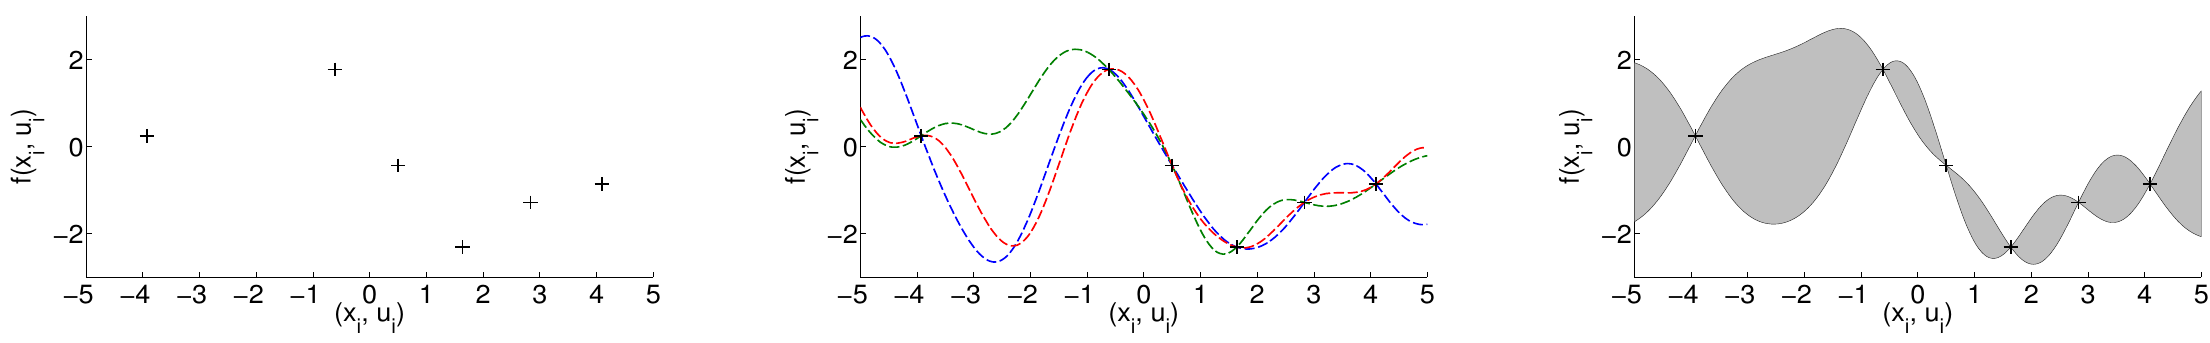
\includegraphics[width=1.0\textwidth]{Chapter1/Figures/PILCO-model-bias.png}
\caption[Model-based bias in reinforcement learning]{Small data set of observed state transitions (left). Several plausible functions that could have generated the data (centre). Posterior distribution showing model uncertainty (right). Reproduced from \citep{deisenroth2011pilco}.}
\label{Fig:model-bias}
\end{figure}

Attempting to further increase PILCO's data-efficiency would require either more informative prior knowledge of the task or extracting more relevant information from the available data. The addition of a exploration scheme would constitute the latter. Many approaches to learning control realise exploration through introducing randomness into action selection. Some approaches comprise a \textit{random exploration phase}, where the controller generates actions randomly, followed by an \textit{exploitation phase}  \citep{thrun1992active}. However, with this strategy once the exploration phase has finished, the agent is unable to adapt to environmental changes during the purely exploitative phase. Others use $\epsilon$-\textit{greedy} policies, which exploit the action with the maximum expected reward most of the time, but with some probability $\epsilon$ a random action is selected \citep{sutton2018reinforcement}. While $\epsilon$-\textit{greedy} approaches encourage learning, for real-world systems, selecting random actions can repeatedly steer the system towards undesirable or dangerous states. In addition, random action selection can be inefficient and often causes the agent to repeatedly return to already well-explored regions of the state-space because exploration is \textit{undirected}.

\textit{Information-directed} or \textit{active} exploration schemes aim to overcome the inefficiencies and risks associated with undirected exploration by driving exploration towards promising states \citep{zhaohan2019directed}. Since PILCO is primarily designed for learning control of mechanical dynamical systems, it is natural to consider this class of exploration algorithm when attempting to further improve its efficiency. Furthermore, since PILCO already quantifies model uncertainty and uses this uncertainty in long-term planning, it is also logical to attempt to incorporate this information in any considered exploration strategies. 

Currently, PILCO evaluates a particular policy by cascading uncertain inputs through the probabilistic model of the transition dynamics. In doing so, it gains insight into the variety of states that could be visited under that policy and is able to make an informed decision about how effective the policy is at achieving high reward. However, this approach only allows PILCO to make decisions based on the total uncertainty as quantified by the model, when in fact there are two sources of uncertainty present in the system. One source of uncertainty is \textit{aleatoric}; that is, representative of unknowns that differ each time the agent encounters the environment. Examples include measurement error or chaotic motion in dynamical systems. The second source of uncertainty is \textit{epistemic}; that is, arising from information that the agent could know in principle but currently does not. In model-based methods, this can be thought of as lack of knowledge about the system's transition dynamics. Hence, epistemic uncertainty can be reduced by observing more data while aleatoric uncertainty is irreducible. This means that in certain situations PILCO could be making decisions based on uncertainty of which the primary constituent is aleatory. In this case, PILCO could be repeatedly selecting policies corresponding to trajectories associated with high aleatoric uncertainty which could be prohibitive to learning.

This dissertation attempts to disentangle and quantify the different sources of uncertainty (aleatoric and epistemic) present in the model of the transition function. Since PILCO is a direct policy search method, the \textit{cost function} is consulted directly, therefore, the influence of the uncertainty in the transition function on the uncertainty in the cost is examined. This is done by using variance as a metric for uncertainty and employing the law of total uncertainty to decompose the total model uncertainty into its constituents. The uncertainties are then estimated, establishing a "gold-standard" Monte-Carlo scheme that propagates trajectories through PILCO's dynamics model. The intention of the research is to lay the foundations for a active-exploration scheme to complement PILCO. 



\nomenclature[z-cif]{$CIF$}{Cauchy's Integral Formula}                                % first letter Z is for Acronyms 
\nomenclature[a-F]{$F$}{complex function}                                                   % first letter A is for Roman symbols
\nomenclature[g-p]{$\pi$}{ $\simeq 3.14\ldots$}                                             % first letter G is for Greek Symbols
\nomenclature[g-i]{$\iota$}{unit imaginary number $\sqrt{-1}$}                      % first letter G is for Greek Symbols
\nomenclature[g-g]{$\gamma$}{a simply closed curve on a complex plane}  % first letter G is for Greek Symbols
\nomenclature[x-i]{$\oint_\gamma$}{integration around a curve $\gamma$} % first letter X is for Other Symbols
\nomenclature[r-j]{$j$}{superscript index}                                                       % first letter R is for superscripts
\nomenclature[s-0]{$0$}{subscript index}                                                        % first letter S is for subscripts

%********************************** %Second Section  *************************************
\section{Related Work} %Section - 1.2
\label{S:related-work}
The use of uncertainty for exploration in reinforcement learning is well-studied, either to improve sample efficiency (\cite{schneider1997exploiting}; \cite{jung2010gaussian}; \cite{deisenroth2011pilco}) or avoid worst-case scenarios and mitigate model bias (\cite{bagnell2001solving}; \cite{nilim2005robust}; \cite{kahn2017uncertainty}; \cite{deisenroth2013gaussian}). While the majority of prior work focuses on estimation methods for either aleatoric or epistemic uncertainty, there has recently been increasing interest in \textit{decomposing} total uncertainty into these two components, which can be used independently in the decision making process.

Prior work that estimates aleatoric uncertainty, or aleatoric risk, has focused on both the randomness in the environment and the agent's actions which lead to stochastic returns. \citet{tamar2016learning} extend temporal difference methods to estimate the variance of the reward distribution by jointly estimating the second moment of the reward-to-go and the value function with a linear function approximator. The authors then derive a relationship between the two estimates to quantify risk. \citet{prashanth2013actor} define variance measures for policies to get risk-sensitive criteria for optimisation which are used alongside actor-critic gradient estimators. Other attempts at creating risk-sensitive agents include the development of distribution reinforcement learning methods which approximate the entire distribution of returns. \citet{morimura2010nonparametric} extend the Bellman equations to include the cumulative return distribution and propose an algorithm that leads to a risk-sensitive reinforcement learning paradigm. \citet{bellemare2017distributional} argue the fundamental importance of the value distribution in reinforcement learning and present theoretical results in both the policy evaluation and control settings. 

Several methods for estimating the epistemic uncertainty have been proposed. \citet{azizzadenesheli2018efficient} and \citet{lipton2018bbq} both present exploration schemes that take into account the epistemic uncertainty by performing Bayesian inference over the parameters that define the value function. \citet{pearce2018bayesian}   estimate parameter uncertainty by regularising the parameters of an ensemble of neural networks about their initialisation values, instead of zero,  and use these estimates to govern the exploration-exploitation process, resulting in steadier, more stable learning. \citet{bellemare2016unifying} take inspiration from the intrinsic motivation literature and quantify the uncertainty of an agent's knowledge through the use of density models. The authors present an algorithm for deriving a pseudo-count of state visits from an arbitrary density model which generalises count-based exploration algorithms to the non-tabular case. Finally, \citet{gal2016dropout} use Bayesian drop-out as an uncertainty estimate and provide a quantitative assessment of model uncertainty in the setting of reinforcement learning.

In the literature, a number of papers tackle the problem of producing estimates for both the aleatoric and epistemic uncertainties. \citet{clements2019estimating} build on the work of \cite{gal2016dropout} and \citet{pearce2018bayesian} and show that the disagreement between only two neural networks is sufficient to produce a low-variance estimate of the epistemic uncertainty on the return distribution and estimate aleatoric risk through a distributional framework. \citet{moerland2017efficient} uses Bayesian drop-out to estimate epistemic uncertainty and aleatoric uncertainty by propagating the return uncertainty through the Bellman equation as a Gaussian distribution. 

There are also a number of papers that consider both kinds of uncertainties in model-based reinforcement learning. \citet{chua2018deep} propose a  probabilistic ensembles with trajectory sampling (PETS) algorithm that combines uncertainty-aware deep network dynamics models with sampling-based uncertainty propagation which has the ability to isolate both sources of uncertainty. Finally, \cite{depeweg2017decomposition} present two uncertainty decompositions for Bayesian neural network models with latent variables that isolate both sources of uncertainty. The first is in the form a variance decomposition and is similar to what is presented in this work and the second in terms of mutual information. The sources of uncertainty are then related to risk-sensitive reinforcement learning.
%!TEX root = ../thesis.tex
%*******************************************************************************
%****************************** Second Chapter *********************************
%*******************************************************************************

\chapter{Methodology}

\ifpdf
    \graphicspath{{Chapter2/Figs/Raster/}{Chapter2/Figs/PDF/}{Chapter2/Figs/}{Chapter2/Figures/}}
\else
    \graphicspath{{Chapter2/Figs/Vector/}{Chapter2/Figs/}{Chapter2/Figures/}}
\fi

\section{PILCO}
PILCO \cite{deisenroth2011pilco} is a model-based indirect policy search method for continuous state $\mathbf{x} \in \mathbb{R}^{D}$ and action $\mathbf{u} \in \mathbb{R}^{F}$ dynamical systems described by
\begin{equation}
    \mathbf{x}_{t+1}=f\left(\mathbf{x}_{t}, \mathbf{u}_{t}\right)+\mathbf{\eta}, \quad \mathbf{\eta} \sim \mathcal{N}\left(\mathbf{0}, \boldgreek{\Sigma}_{\eta}\right)
\end{equation}
where the transition dynamics $f$ of the system are unknown. The objective is to find a deterministic \textit{controller/policy} $\pi : \mathbf{x} \mapsto \pi(\mathbf{x}, \boldgreek{\theta})=\mathbf{u}$ such that the expected return   \cite{deisenroth2013gaussian}
\begin{equation}
    J^{\pi}(\theta)=\sum_{t=0}^{T} \mathbb{E}_{\mathbf{x}_{t}}\left[c\left(\mathbf{x}_{t}\right)\right], \quad \mathbf{x}_{0} \sim \mathcal{N}\left(\boldgreek{\mu}_{0}, \boldgreek{\Sigma}_{0}\right)
    \label{Eq:PILCO-expected-return}
\end{equation}
is minimised after following $\pi$ for $T$ steps. The policy is parametrised by $\mathbf{\theta}$, which take the form of nonlinear RBF networks, where $\mathbf{\theta}$ are the weights and features, or linear-affine transformations, where $\mathbf{\theta}$ are the weights matrix and bias terms. The \textit{cost} $c(\mathbf{x}_{t})$, or negative reward, of being in state $\mathbf{x}$ at time $t$ is the generalised binary saturating cost \cite{deisenroth2013gaussian}
\begin{equation}
    c(\mathbf{x}_{t})=1-\exp \left(-\frac{1}{2 \sigma_{c}^{2}} d\left(\mathbf{x}_{t}, \mathbf{x}_{\text { target }}\right)^{2}\right) \in[0,1]
    \label{Eq:PILCO-cost-function}
\end{equation}
which exclusively penalises the Euclidean distance $d$ from the current state $\mathbf{x}_{t}$ to the target state $\mathbf{x}_{\text { target }}$. $c(\mathbf{x}_{t})$ is locally quadratic and saturates at 1 for large differences between the current state and target state. The saturation distance is controlled by the width parameter $\sigma_{c}$.

\subsection{GP Model Learning}
\label{PILCO:GP-model-learning}
The system dynamics are modelled as a probabilistic Gaussian Process (GP). Tuples of the state and control vectors $\left(\mathbf{x}_{t}, \mathbf{u}_{t}\right)\in \mathbb{R}^{D+F}$ serve as training inputs and differences $\Delta_{t}=\mathbf{x}_{t+1}-\mathbf{x}_{t}+\varepsilon \in \mathbb{R}^{D},\quad \varepsilon \sim \mathcal{N}\left(0, \boldgreek{\Sigma}_{\varepsilon}\right)$ as training targets. Conditionally independent GP's are trained for for each target dimension \cite{deisenroth2010efficient}. The dynamics model provides a \textit{one-step} prediction \cite{deisenroth2011pilco}
\begin{equation}
    p\left(\mathbf{x}_{t+1} | \mathbf{x}_{t}, \mathbf{u}_{t}\right)=\mathcal{N}\left(\mathbf{x}_{t} | \mu_{t}, \boldgreek{\Sigma}_{t}\right)
    \label{Eq:PILCO-one-step-1}
\end{equation}
\begin{equation}
    \mu_{t+1}=\mathbf{x}_{t}+\mathbb{E}_{f}\left[\Delta_{t}\right]
    \label{Eq:PILCO-one-step-2}
\end{equation}
\begin{equation}
    \boldgreek{\Sigma}_{t+1}=\operatorname{var}_{f}\left[\Delta_{t}\right]
    \label{Eq:PILCO-one-step-3}
\end{equation}
where the mean $\mu$ of the state $\mathbf{x}_{t+1}$ is obtained through addition of the current state $\mathbf{x}_{t}$ with the one-step difference prediction $\mathbb{E}_{f}\left[\Delta_{t}\right]$. A GP is defined completely by a mean function $m(\cdot)$ and a positive semidefinite covariance function $K(\cdot,\cdot)$. PILCO follows the common practice of setting the mean prior function to zero and uses the \textit{stationary} anisotropic squared exponential covariance function
\begin{equation}
    k\left(\tilde{\mathbf{x}}_{i}, \tilde{\mathbf{x}}_{j}\right)=\sigma_{0}^{2} \exp \left(-\frac{1}{2}\left(\tilde{\mathbf{x}}_{i}-\tilde{\mathbf{x}}_{j}\right)^{\top} \boldgreek{\Lambda}^{-1}\left(\tilde{\mathbf{x}}_{i}-\tilde{\mathbf{x}}_{j}\right)\right)
    \label{Eq:PILCO-sq-exponential-covariance}
\end{equation}
where $\tilde{\mathbf{x}} = \left[\mathbf{x}\quad\mathbf{u}\right]^{T}$ is the state-action vector, $\boldgreek{\Lambda} =\operatorname{diag}\left(\left[\ell_{1}^{2}, \ldots, \ell_{D+F}^{2}\right]\right)$ depends on the characteristic lengthscales and $\sigma_{0}$ is the variance of the latent function \cite{deisenroth2013gaussian}. The lengthscales determine the speed that the covariance decays with the distance between inputs \cite{quia2010sparse}.

\subsection{Policy Evaluation}
\label{PILCO:policy-evaluation}
PILCO evaluates a given policy by predicting the state evolution over the course of an episode. This is accomplished by propagating uncertain inputs through the dynamics model, using the one-step predictions (Eqs. \ref{Eq:PILCO-one-step-1} - \ref{Eq:PILCO-one-step-3}), to obtain $p\left(\mathbf{x}_{1} | \pi\right), \ldots, p\left(\mathbf{x}_{T} | \pi\right)$ from a given start state distribution $p\left(\mathbf{x}_{0}\right)$. Predicting $\mathbf{x}_{t+1}$ from $p(\mathbf{x}_{t})$ requires evaluation of the predictive distribution over state differences
\begin{equation}
    p\left(\Delta_{t}\right)=\iint p\left(f\left(\tilde{\mathbf{x}}_{t}\right) | \left(\tilde{\mathbf{x}}_{t}\right)\right) p\left(\tilde{\mathbf{x}}_{t}\right) \mathrm{d} f \mathrm{d} \tilde{\mathbf{x}}_{t},
    \label{Eq:PILCO-predictive-state-differences}
\end{equation}
by integrating out the random function of the GP distribution and the random variable $\tilde{\mathbf{x}}_{t}$. Here $p\left(\tilde{\mathbf{x}}_{t}\right)=p\left(\mathbf{x}_{t}, \mathbf{u}_{t}\right)$ is the joint state-action distribution. Since the predictive distribution in Eq. \ref{Eq:PILCO-predictive-state-differences} is analytically intractable for uncertain inputs, it is approximated as a Gaussian distribution using \textit{moment matching} (see Fig. \ref{Fig:moment-matching}). This approximation ensures that the state distribution is given by $p\left(\tilde{\mathbf{x}}_{t}\right)=\mathcal{N}\left(\tilde{\mathbf{x}}_{t} | \tilde{\mathbf{\mu}}_{t}, \tilde{\boldgreek{\Sigma}}_{t}\right)$ for all $t$. This, alongside the choice of cost function (Eq. \ref{Eq:PILCO-cost-function}) enables the expected return (Eq. \ref{Eq:PILCO-expected-return}) to be evaluated analytically according to
\begin{equation}
    \mathbb{E}_{\mathbf{x}_{t}}\left[c\left(\mathbf{x}_{t}\right)\right]=\int c\left(\mathbf{x}_{t}\right) \mathcal{N}\left(\mathbf{x}_{t} | \boldgreek{\mu}_{t}, \boldgreek{\Sigma}_{t}\right) \mathrm{d} \mathbf{x}_{t}
\end{equation}
for $t=1,\dots,T$.

\begin{figure}
\centering    
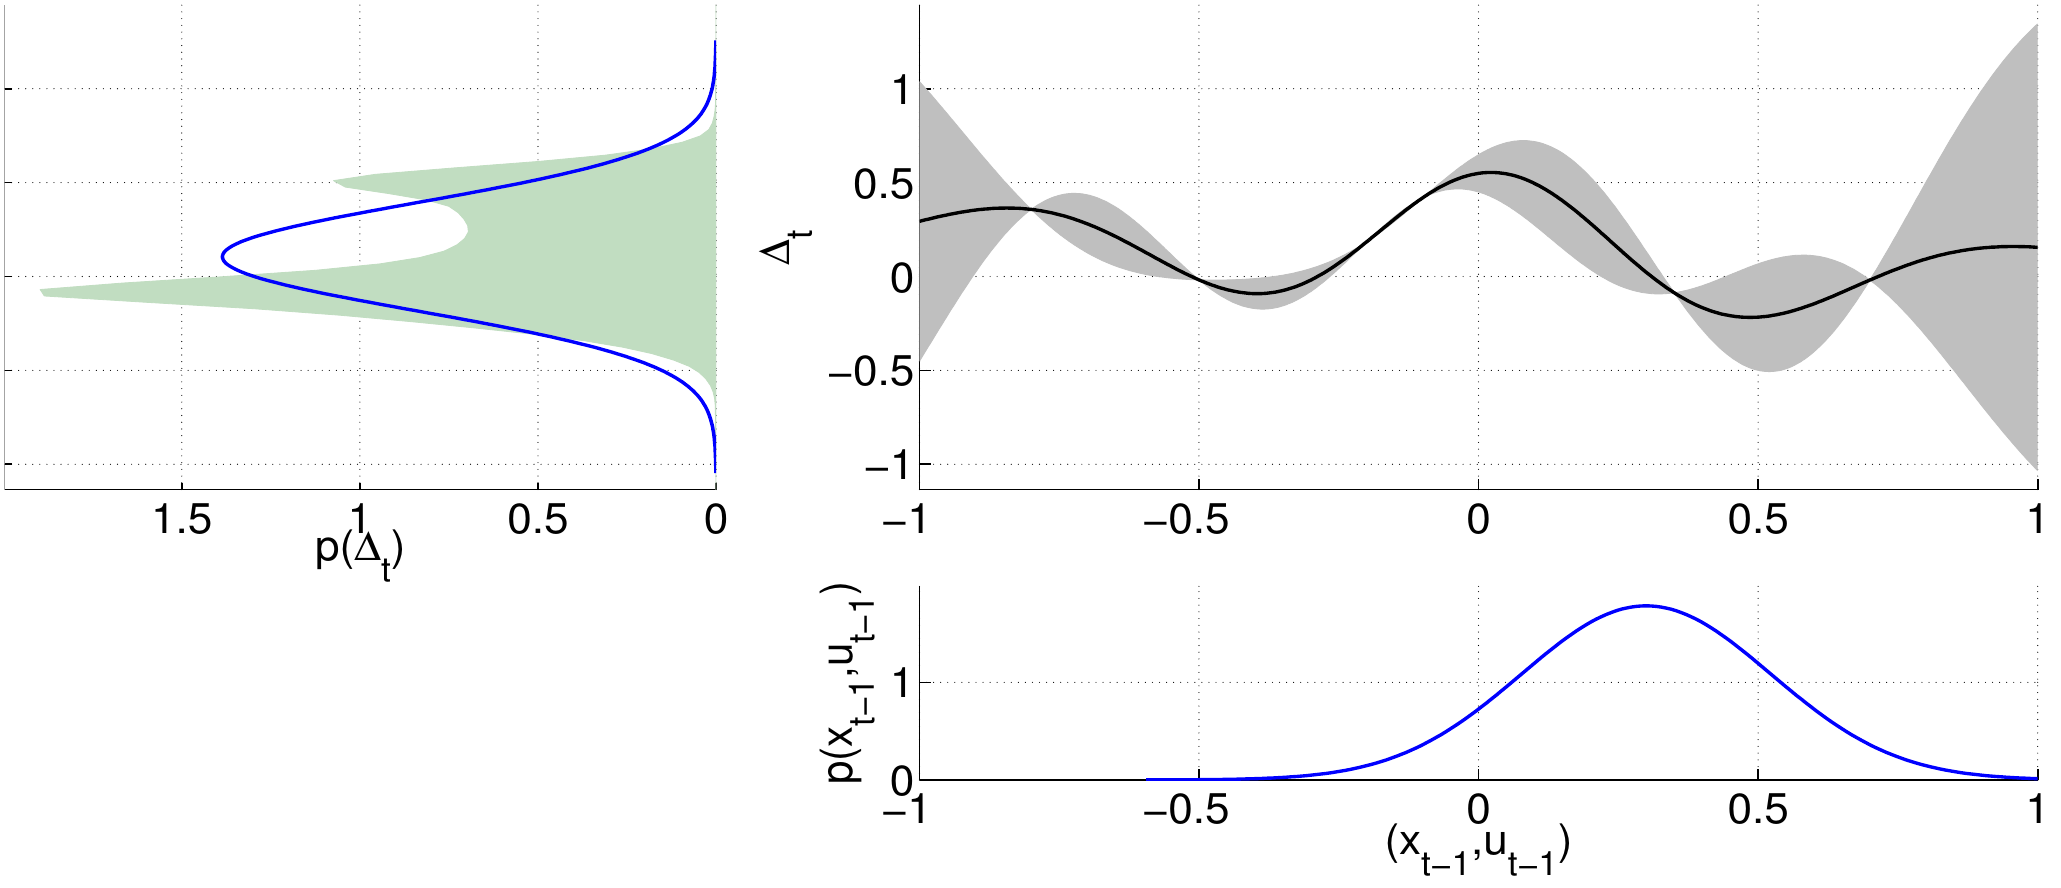
\includegraphics[width=1.0\textwidth]{PILCO-moment-matching.png}
\caption[Propagating an uncertain input through the GP dynamics model]{Propagating an uncertain input through the GP dynamics model (upper right panel). The input distribution $p(x_{t-1},u_{t-1})$, assumed to be Gaussian (lower right panel), is propagated through the dynamics model yielding the shaded distribution $p(\Delta_{t})$. The shaded distribution is then approximated by a Gaussian with the same mean and variance (upper left panel). Reproduced from \cite{deisenroth2011pilco}.}
\label{Fig:moment-matching}
\end{figure}

\subsection{Policy Improvement}
\label{PILCO:policy-improvement}
PILCO is an indirect policy search method and does not require an explicit value function model. Instead it learns a \textit{parametrised policy} that can select actions without consulting a value function. Due to the moment matching approximation, the state distribution is considered to be Gaussian $p\left(\tilde{\mathbf{x}}_{t}\right)=\mathcal{N}\left(\tilde{\mathbf{x}}_{t} | \tilde{\mathbf{\mu}}_{t}, \tilde{\boldgreek{\Sigma}}_{t}\right)$ for all $t$, where $\tilde{\mathbf{x}}_{t} = (\mathbf{x}_{t},\mathbf{u}_{t})$. The control signal  $\mathbf{u}_{t-1} = \pi\left(\mathbf{x}_{t-1}, \theta\right)$ is a function of the state, and hence the next state is also functionally dependent on the mean $\mu_{u}$ and covariance $\boldgreek{\Sigma}_{u}$ of the control signal. This relationship allows the gradients of the expected return $J^{\pi}$, with respect to the policy parameters $\boldgreek{\theta}$, to be computed analytically. The policy parameters are then learned to \textit{maximise} performance (\textit{minimise} cost) for a given task, so their updates approximate gradient \textit{descent} in $J$ \cite{sutton2018reinforcement}:
\begin{equation}
    \boldgreek{\theta}_{t+1}=\boldgreek{\theta}_{t} - \alpha\nabla J^{\pi}\left(\boldgreek{\theta_{t}}\right),
\end{equation}
where $\alpha$ is the learning rate. For a more thorough explanation of PILCO see \cite{deisenroth2011pilco}\cite{deisenroth2010efficient}\cite{deisenroth2013gaussian}. Algorithm \ref{PILCO:algorithm-1} provides an overview of PILCO.

\begin{algorithm}
\caption{PILCO}\label{PILCO:algorithm-1}
\begin{algorithmic}[1]
\State \textbf{init:} Sample controller parameters $\boldgreek{\theta} \sim \mathcal{N}\left(\mathbf{0},\mathbf{I}\right)$
\Repeat{}
\State Learn probabilistic GP dynamics model using all environment data \Comment{Sec \ref{PILCO:GP-model-learning}}
\Repeat{}
\State Approximate inference for policy evaluation: $J^{\pi}\left(\theta\right)$ \Comment{Sec \ref{PILCO:policy-evaluation}}
\State Gradient-based policy improvement: $\mathrm{d} J^{\pi}(\boldsymbol{\theta}) / \mathrm{d} \boldsymbol{\theta}$ \Comment{Sec \ref{PILCO:policy-improvement}}
\State Update parameters $\boldgreek{\theta}$\Comment{CG or L-BFGS}
\Until convergence; \textbf{return} $\boldgreek{\theta}^{*}$
\State Set $\pi^{*} \gets \pi\left(\theta^{*}\right)$
\State  Apply $\pi^{*}$ to environment and record data
\Until task learned \Comment{modified from \cite{deisenroth2011pilco}}
\end{algorithmic}
\end{algorithm}

\section{Approximating PILCO's GP}
At the heart of the Monte Carlo uncertainty approximation is the need for one-step predictions using a function sampled from the posterior distribution of PILCO's dynamics model. The use of the squared exponential covariance function in PILCO's GP corresponds to a Bayesian linear regression model with an infinite number of basis functions \cite{williams2006gaussian}. This means drawing a representative function requires an infinite number of weights since each basis function is accompanied by its own weight. To overcome this issue, a finite-weight stationary trigonometric Bayesian regression model \cite{quia2010sparse} is used to approximate PILCO's GP. In addition to solving the sampling issue, this model provides other advantages. First, the periodicity of the trigonometric basis functions means that one does not need to explicitly specify the mean for each basis function. Second, a direct GP implementation has practical limitations with regards to computational and memory requirements, which scale as $\mathcal{O}(n^{2})$ and $\mathcal{O}(n^{3})$, respectively. The trigonometric model has computational requirements of $\mathcal{O}(nm^{2})$ and memory requirements of $\mathcal{O}(nm)$ where $m<<n$ \cite{quia2010sparse}, which are typical values for sparse GP approximations \cite{quinonero2005unifying}. The largest PILCO environment used for this research (cart double pendulum) generates approximately $4k$ data points. The model is first introduced here in a traditional treatment of Bayesian linear regression. Section \ref{S:one-step-predictions} relates the model to PILCO's one-step predictions. Finally, section \ref{S:sparse-approximation} shows that the model can be viewed as a sparse stationary GP that can approximate any full GP.

The model consists of a linear combination of trigonometric functions \cite{quia2010sparse}
\begin{equation}
    f(\mathbf{x})=\sum_{r=1}^{m} a_{r} \cos \left(2 \pi \mathbf{s}_{r}^{\top} \mathbf{x}\right)+b_{r} \sin \left(2 \pi \mathbf{s}_{r}^{\top} \mathbf{x}\right)
    \label{Eq:Model-trigonometric-model}
\end{equation}
where $\mathbf{s}_{r}$ is a $D$-dimensional vector of spectral frequencies shared by each pair of basis functions while $a_{r}$ and $b_{r}$ are amplitude parameters which are independent for each basis function (see Sec \ref{S:sparse-approximation} for selecting spectral frequencies). The amplitudes have independent Gaussian priors with linearly scaled variances 
\begin{equation}
    a_{r} \sim \mathcal{N}\left(0, \frac{\sigma_{0}^{2}}{m}\right), \quad b_{r} \sim \mathcal{N}\left(0, \frac{\sigma_{0}^{2}}{m}\right)
\end{equation}
where $m$ are the number basis functions. The frequencies function as deterministic parameters and the amplitudes are treated in a Bayesian fashion. For this, the model is packaged as the dot product between the set of amplitudes and the basis functions 
\begin{equation}
    f(\mathbf{x}, \mathbf{w}) = \mathbf{w}^{\top} \varphi\left(\mathbf{x}\right)
\end{equation}
where $\mathbf{x}$ is a $D$-dimensional input variable, $\mathbf{w}=\left[a_{1}, b_{1}, \dots, a_{m}, b_{m}\right]^{\top}$ are the model weights and
\begin{equation}
    \varphi(\mathbf{x})=\left[\cos \left(2 \pi \mathbf{s}_{1}^{\top} \mathbf{x}\right)\quad \sin \left(2 \pi \mathbf{s}_{1}^{\top} \mathbf{x}\right) \quad\ldots\quad \cos \left(2 \pi \mathbf{s}_{m}^{\top} \mathbf{x}\right) \quad \sin \left(2 \pi \mathbf{s}_{m}^{\top} \mathbf{x}\right)\right]^{\top}.
\end{equation}
The model targets are now assumed to have been generated by the function $f(\mathbf{x}, \mathbf{w})$ and independently corrupted by additive Gaussian noise of constant variance $\sigma_{n}^{2}$
\begin{equation}
    y = f(\mathbf{x}, \mathbf{w}) + \varepsilon, \quad \varepsilon \sim \mathcal{N}\left(0,\sigma_{n}^{2}\right).
\end{equation}
This can be written as 
\begin{equation}
    p(y | \mathbf{x}, \mathbf{w}, \sigma^{2}_{n})= \mathcal{N}\left(y | f(\mathbf{x}, \mathbf{w}), \sigma^{2}_{n}\right).
    \label{Eq:Model-one-value-likelihood}
\end{equation}
For a dataset of model inputs $\mathbf{X}=\left\{\mathbf{x}_{1}, \dots, \mathbf{x}_{N}\right\}$ with corresponding target values $\mathbf{y}=\{y_{1}, \dots, y_{N}\}$ and assuming that these data points have been drawn independently from $\mathcal{N}(y|f(\mathbf{x}, \mathbf{w}), \sigma^{2}_{n})$, the likelihood function is
\begin{equation}
    p(\mathbf{y} | \mathbf{X}, \mathbf{w}, \sigma^{2}_{n})=\prod_{i=1}^{N} \mathcal{N}\left(y_{i} | \mathbf{w}^{\top} \varphi\left(\mathbf{x}_{i}\right), \sigma^{2}_{n}\right).
\end{equation}
The posterior distribution over the model weights is proportional to the product of the likelihood function and the prior. Since the Gaussian prior is conjugate, the posterior distribution is also Gaussian (see Appendix \ref{A:derivation-posterior-over-weights} for derivation)
\begin{equation}
    q(\mathbf{w} | \mathbf{y}, \mathbf{X}, \sigma_{0}^{2}, \sigma_{n}^{2})=\mathcal{N}\left(\mathbf{w} | \mathbf{\mu_{\mathbf{w}}}, \mathbf{A}^{-1}\right)
    \label{Eq:Model-posterior-over-weights}
\end{equation}
where the posterior mean $\mu_{\mathbf{w}}$ and precision matrix $A$ are
\begin{equation}
    \mathbf{\mu_{\mathbf{w}}}=\frac{1}{\sigma_{n}^{2}} \mathbf{A}^{-1} \Phi \mathbf{y}
\end{equation}
\begin{equation}
    \mathbf{A} =\frac{1}{\sigma_{n}^{2}} \Phi \Phi^{\top} + \frac{m}{\sigma_{0}^{2}} \mathbf{I}_{2m}.
\end{equation}
Here, $\Phi = \left[\varphi(\mathbf{x}_{1}), \dots , \varphi(\mathbf{x}_{N})\right]$ is the $2m$ by $N$ \textit{design matrix}.

To make a prediction $y_{*}$ for a new input value $\textbf{x}_{*}$ requires evaluation of the predictive distribution, defined by
\begin{equation}
   p(y_{*} | \mathbf{y},\mathbf{X},\mathbf{x}_{*}, \sigma_{0}^{2}, \sigma_{n}^{2})=\int p(y_{*} | \mathbf{x}_{*}, \mathbf{w}, \sigma_{n}^{2}) q(\mathbf{w} | \mathbf{y}, \mathbf{X}, \sigma_{0}^{2}, \sigma_{n}^{2}) \mathrm{d} \mathbf{w}
\end{equation}
where the conditional distribution of the target variable $p(y_{*} | \mathbf{x}_{*}, \mathbf{w}, \sigma_{n}^{2})$ is defined by Eq. \ref{Eq:Model-one-value-likelihood} and the posterior distribution over the weights is given by Eq. \ref{Eq:Model-posterior-over-weights}. The predictive distribution for a single input is (see Appendix \ref{A:derivation-predictive-distribution} for derivation)
\begin{equation}
    p(y_{*} | \mathbf{y},\mathbf{X},\mathbf{x}_{*}, \sigma_{0}^{2}, \sigma_{n}^{2}) = \mathcal{N}\left(y_{*} | \mathbf{\mu}_{y_{*}}, \sigma_{y_{*}}^{2}\right)
    \label{Eq:Model-predicitive-distribution}
\end{equation}
where
\begin{equation}
    \mu_{y_{*}} = \frac{1}{\sigma_{n}^{2}}\varphi(\mathbf{x}_{*})^{\top} \mathbf{A}^{-1} \Phi \mathbf{y}
\end{equation}
\begin{equation}
    \sigma_{y_{*}}^{2}=\sigma_{n}^{2} + \varphi(\mathbf{x}_{*})^{\top}\mathbf{A}^{-1}\varphi(\mathbf{x}_{*}).
    \label{Eq:Model-predictive-variance}
\end{equation}
\paragraph{A note on model uncertainty:} The predictive variance (Eq. \ref{Eq:Model-predictive-variance}) consists of two terms. The first represents the noise present on the data while the second quantifies the uncertainty associated with the model weights $\textbf{w}$ \cite{bishop2006pattern}. The latter is particularly relevant to this research and will be expanded on in Section \ref{S:disentangling-uncertainty}. As more data is observed, the model becomes increasingly confident and consequently the posterior distribution narrows due to contraction of the second term. \citet{qazaz1997upper} show that $\sigma_{y_{*}(N+1)}^{2} \leqslant \sigma_{y_{*}(N)}^{2}$ while in the limit $N \to \infty$ the second term of Eq. \ref{Eq:Model-predictive-variance} reduces to zero. In this case the model has full confidence in the weights and the predictive variance's sole contributor is the data noise governed by the $\sigma_{n}^2$ term.

\subsection{One-Step Predictions}
\label{S:one-step-predictions}
The trigonometric basis function model used to approximate PILCO's GP is also trained with tuples of the state and control vectors $\tilde{\mathbf{x}}_{t}=\left(\mathbf{x}_{t}, \mathbf{u}_{t}\right)\in \mathbb{R}^{D+F}$ as training inputs and state differences $\Delta_{t}=\mathbf{x}_{t+1}-\mathbf{x}_{t}+\varepsilon,\quad \varepsilon \sim \mathcal{N}\left(0, \boldgreek{\Sigma}_{\varepsilon}\right)$ as targets. However, while the one-step predictions generated by PILCO's GP dynamics model are produced by the posterior predictive distribution, for the uncertainty estimations in Sec \ref{S:disentangling-uncertainty}, functions drawn from the posterior distribution over the model weights are used to make one-step predictions. For this, first a set of $2m$ weights is drawn from the posterior distribution $\mathbf{w} \sim q(\mathbf{w})$ (Eq. \ref{Eq:Model-posterior-over-weights}) where the conditioning variables are dropped for brevity. The one-step predictions are then computed with
\begin{equation}
    \mathbf{x}_{t+1}
    = \mathbf{x}_{t} + \Delta_{t} \\
    =\mathbf{x}_{t}+\mathbf{w}^{\top}\varphi(\tilde{\mathbf{x}}_{t}).
    \label{Eq:model-posterior-one-step}
\end{equation}

\subsection{A Sparse Approximation to the Full GP}
\label{S:sparse-approximation}
This section follows the treatment in \cite{quia2010sparse} and relates the trigonometric basis function model of the previous section to a full GP by creating a sparse representation of the stationary covariance function. GP regression is a probabilistic, non-parametric Bayesian approach that is completely specified by a mean function and covariance function \cite{williams2006gaussian}
\begin{equation}
    \begin{aligned} 
    m(\mathbf{x}) 
    &=\mathbb{E}[f(\mathbf{x})] \\ k\left(\mathbf{x}_{i}, \mathbf{x}_{j}\right) &=\mathbb{E}\left[(f(\mathbf{x}_{i})-m(\mathbf{x}_{i}))\left(f\left(\mathbf{x}_{j}\right)-m\left(\mathbf{x}_{j}\right)\right)\right]. 
    \end{aligned}
\end{equation}
Similar to the PILCO GP, a zero mean function $m(\mathbf{x})=0$ and stationary squared exponential covariance function
\begin{equation}
    k\left(\mathbf{x}_{i}, \mathbf{x}_{j}\right)=k\left(\mathbf{x}_{i}-\mathbf{x}_{j}\right)=k(\tau)
    \label{Eq:stationary-covariance-tau}
\end{equation}
are considered (see Eq \ref{Eq:PILCO-sq-exponential-covariance}). A stationary covariance function is a function $\boldgreek{\tau} = \mathbf{x}_{i}-\mathbf{x}_{j}$ that depends only on the difference between inputs. Now considering the trigonometric basis function model in Eq \ref{Eq:Model-trigonometric-model}. Under the prior, the distribution over functions is Gaussian with zero mean and stationary covariance function \cite{quia2010sparse}
\begin{equation}
    k\left(\mathbf{x}_{i}, \mathbf{x}_{j}\right)=\frac{\sigma_{0}^{2}}{m} \varphi\left(\mathbf{x}_{i}\right)^{\top} \varphi\left(\mathbf{x}_{j}\right)=\frac{\sigma_{0}^{2}}{m} \sum_{r=1}^{m} \cos \left(2 \pi \mathbf{s}_{r}^{\top}\left(\mathbf{x}_{i}-\mathbf{x}_{j}\right)\right).
    \label{Eq:phi-to-covariance-relationship}
\end{equation}
\begin{theorem}[Bochner's theorem]
\label{T:bochners-theorem}
A complex-valued function $k$ on $\mathbb{R}^{D}$ is the
covariance function of a weakly stationary mean square continuous complex-valued random process on $\mathbb{R}^{D}$ if and only if it can be represented as
\begin{equation}
    k(\boldgreek{\tau})=\int_{\mathbb{R}^{D}} e^{2 \pi i \mathbf{s} \cdot \boldgreek{\tau}} d \mu_{fm}(\mathbf{s})
\end{equation}
where $\mu_{fm}$ is a positive finite measure. \Comment{Quoted from \cite{stein1999interpolation}}
\end{theorem}
If $\mu_{fm}$ has a probability density $S(\mathbf{s})$ then $S$ is the \textit{spectral density} associated with $k$ \cite{williams2006gaussian} and is proportional to a probability measure $S(\mathbf{s}) \propto p_{S}(\mathbf{s})$. The proportionality constant can be obtained by evaluating the covariance function in Eq \ref{Eq:stationary-covariance-tau} at $\boldgreek{\tau}=\mathbf{0}$ to give 
\begin{equation}
    S(\mathbf{s})=k(\mathbf{0}) p_{S}(\mathbf{s})=\sigma_{0}^{2} p_{S}(\mathbf{s}).
\end{equation}
Should $S(\mathbf{s})$ exist, according to the Wiener-Khintchine theorem \cite{chatfield1989timeseries}, the covariance function and the spectral density form a Fourier pair
\begin{equation}
    k(\boldgreek{\tau})=\int S(\mathbf{s}) e^{2 \pi i \mathbf{s} \cdot \boldgreek{\tau}} d \mathbf{s}, \quad S(\mathbf{s})=\int k(\boldgreek{\tau}) e^{-2 \pi i \mathbf{s} \cdot \tau} d \boldgreek{\tau}.
\end{equation}
Since $S(\mathbf{s})$ is proportional to a multivariate probability density in $\mathbf{s}$ the covariance function can be rewritten as an expectation with respect to the probability measure $p_{S}(\mathbf{s})$ 
\begin{equation}
    \begin{aligned}
    k(\boldgreek{\tau})
    &=\int_{\mathbb{R}^{D}} e^{2 \pi i \mathbf{s}^{\top}\left(\mathbf{x}_{i}-\mathbf{x}_{j}\right)} S(\mathbf{s}) \mathrm{d} \mathbf{s}\\
    &=\sigma_{0}^{2} \int_{\mathbb{R}^{D}} e^{2 \pi i \mathbf{s}^{\top} \mathbf{x}_{i}}\left(e^{2 \pi i \mathbf{s}^{\top} \mathbf{x}_{j}}\right)^{*} p_{S}(\mathbf{s}) d \mathbf{s} \\ 
    &=\sigma_{0}^{2} \mathbb{E}_{p_{S}(\mathbf{s})}\left[e^{2 \pi i \mathbf{s}^{\top} \mathbf{x}_{i}}\left(e^{2 \pi i \mathbf{s}^{\top} \mathbf{x}_{j}}\right)^{*}\right] \end{aligned}
    \label{Eq:k-tau-expectation-wrt-ps}
\end{equation}
where the superscript asterisk denotes complex conjugation. The result in Eq. \ref{Eq:k-tau-expectation-wrt-ps} can be estimated by simple Monte Carlo. Since the spectral density is symmetric about zero, sampling frequency pairs $\{\mathbf{s}_{r},-\mathbf{s}_{r}\}$ preserves the exact expansion where the imaginary terms cancel
\begin{equation}
    \begin{aligned} 
    k\left(\mathbf{x}_{i}, \mathbf{x}_{j}\right) 
    & \simeq \frac{\sigma_{0}^{2}}{2 m} \sum_{r=1}^{m}\left[e^{2 \pi i \mathbf{s}_{r}^{\top} \mathbf{x}_{i}}\left(e^{2 \pi i \mathbf{s}_{r}^{\top} \mathbf{x}_{j}}\right)^{*}+\left(e^{2 \pi i \mathbf{s}_{r}^{\top} \mathbf{x}_{i}}\right)^{*} e^{2 \pi i \mathbf{s}_{r}^{\top} \mathbf{x}_{j}}\right] \\ &=\frac{\sigma_{0}^{2}}{m} \operatorname{Re}\left[\sum_{r=1}^{m} e^{2 \pi i \mathbf{s}_{r}^{\top} \mathbf{x}_{i}}\left(e^{2 \pi i \mathbf{s}_{r}^{\top} \mathbf{x}_{j}}\right)^{*}\right] \\
    &=\frac{\sigma_{0}^{2}}{m} \sum_{r=1}^{m} \cos \left(2 \pi \mathbf{s}_{r}^{\top}\left(\mathbf{x}_{i}-\mathbf{x}_{j}\right)\right).
    \end{aligned}
\end{equation}
Here, $Re$ is the real part of the complex number and the finite set of Monte Carlo frequencies $\mathbf{s}_{r}$, called \textit{spectral points}, are sampled from $p_{S}(\mathbf{s})$. This result shows that Eq. \ref{Eq:phi-to-covariance-relationship} is recovered by sparsifying the stationary covariance function of a full GP meaning that the trigonometric basis function model of the previous section is indeed a sparse spectrum Gaussian process. 

Taking the Fourier transform of the squared exponential covariance function used in PILCO's GP dynamics model gives a probability density of multivariate Gaussian form
\begin{equation}
    p_{S}(\mathbf{s})=\frac{1}{k(\mathbf{0})} \int_{\mathbb{R}^{D}} e^{-2 \pi i \mathbf{s}^{\top} \tau} k(\mathbf{\tau}) d \tau=\sqrt{|2 \pi \Lambda|} \exp \left(-2 \pi^{2} \mathbf{s}^{\top} \Lambda \mathbf{s}\right)
    \label{Eq:Gaussian-spectral-points-sample}
\end{equation}
from which the spectral points are drawn for the Monte Carlo estimate of $k(\mathbf{x}_{i},\mathbf{x}_{j})$. 

\subsection{Hyperparameter Optimisation}
In a fully Bayesian treatment of the trigonometric basis function model one would introduce priors over $\sigma_{0}^2$ and $\sigma_{n}^2$ and marginalise with respect to both the hyperparameters and the weights $\mathbf{w}$ to make predictions. However, while marginalisation over either the hyperparameters or the weights is plausible, complete marginalisation over both is analytically intractable \cite{bishop2006pattern}. Instead, here the hyperparameters are learned through optimising the log marginal likelihood (see Appendix ?? for derivation)
\begin{equation}
    \log p\left(\mathbf{y}|\boldgreek{\theta}\right) = -\frac{1}{2\sigma_{n}^{2}}\left[\mathbf{y}^{\top}\mathbf{y} - \frac{1}{\sigma_{n}^{2}}\mathbf{y}^{\top}\Phi^{\top}\mathbf{A}^{-1}\Phi\mathbf{y}\right] - \frac{1}{2}\log|\mathbf{A}| + m\log\frac{m}{\sigma_{0}^{2}} - \frac{n}{2}\log2\pi\sigma_{n}^{2}
\end{equation}
with respect to the hyperparameters $\sigma_{0}^{2}$, $\sigma_{n}^{2}$, and the lengthscales $\{\ell_{1},\dots,\ell_{D}\}$ governing each input dimension. The hyperparameters are initialised to the variance of $\{y_{i}\}$ and $\sigma_{0}^2/4$, and half the ranges of the input dimensions for the lengthscales \cite{quia2010sparse}. One hundred sets of $m\times D$ spectral points are drawn from Eq. \ref{Eq:Gaussian-spectral-points-sample} and the log marginal likelihood is evaluated for each set. The set corresponding to the highest log marginal likelihood value are kept. No further optimisation is performed on the spectral points \textbf{(WHY?)}.


\section{Disentangling Sources of Uncertainty}
\label{S:disentangling-uncertainty}
1. change the model section to delta and state-action representations. 
2. Start this section with a discussion on model bias and how the uncertainty in the transition function does stuff (from ppilco paper). 
Introduce the predictive distribution and the sources of uncertainty. Talk about how the uncertainty is in the weights etc.
3. Well, we only really care about the uncertainty that affects the loss..
4. derive uncertainty decomposition

The one-step predictions described in Sec \ref{S:one-step-predictions} use functions drawn from the posterior distribution over the model weights. Although not used for the one-step predictions, the predictive distribution of the approximate GP model is still important because ultimately it is the uncertainty in the .

In the trigonometric basis function model chosen to approximate the GP, the predicative distribution over state differences 

PILCO selects a policy to execute that maximises the expected reward, given its current beliefs. 

Interested in the impact of the different types of uncertainties on PILCO's loss function. Need to bring in the concepts of controller that yields a low cost and a high epistemic uncertainty maybe?
Reproduce the model predictive distribution and speak about the different sources of uncertainty. Relate this back to the note on uncertainty in the model section.
Explain what aleatoric and epistemic uncertainty is and that one can be reduced with more data.
Derive the uncertainty decomposition and discuss in an intuitive way how it actually works, i.e. the variance produced by the different draws from the posterior have a variance that can be measured.
\subsection{Variance vs Mutual Information}
\section{Monte-Carlo Uncertainty Estimates}

PILCO evaluates a given policy by propagating uncertain inputs through the GP dynamics model to obtain long-term predictions of the state evolution $p(\mathbf{x}_{1}|\pi),...,p(\mathbf{x}_{T}|\pi)$. While the predictive distribution over state differences in Eq. \ref{Eq:PILCO-predictive-state-differences} is analytically intractable for uncertain inputs, it is tractable for a single or series of deterministic inputs \textbf{*need to check this is correct}. So too is the approximating model 

The predictive distribution over state differences with uncertain inputs is intractable. So here the exact predictive is a pproximated by Monte Carlo.



\clearpage

\tochide\section{Hidden section}



\begin{landscape}

\section*{Subplots}
I can cite Wall-E (see Fig.~\ref{fig:WallE}) and Minions in despicable me (Fig.~\ref{fig:Minnion}) or I can cite the whole figure as Fig.~\ref{fig:animations}


\begin{figure}
  \centering
  \begin{subfigure}[b]{0.3\textwidth}
    \includegraphics[width=\textwidth]{TomandJerry}
    \caption{Tom and Jerry}
    \label{fig:TomJerry}   
  \end{subfigure}             
  \begin{subfigure}[b]{0.3\textwidth}
    \includegraphics[width=\textwidth]{WallE}
    \caption{Wall-E}
    \label{fig:WallE}
  \end{subfigure}             
  \begin{subfigure}[b]{0.3\textwidth}
    
\includegraphics[width=\textwidth]{minion}
    \caption{Minions}
    \label{fig:Minnion}
  \end{subfigure}
  \caption{Best Animations}
  \label{fig:animations}
\end{figure}


\end{landscape}

%!TEX root = ../thesis.tex
%*******************************************************************************
%****************************** Third Chapter **********************************
%*******************************************************************************
\chapter{Outcomes}

% **************************** Define Graphics Path **************************
\ifpdf
    \graphicspath{{Chapter3/Figs/Raster/}{Chapter3/Figs/PDF/}{Chapter3/Figs/}}
\else
    \graphicspath{{Chapter3/Figs/Vector/}{Chapter3/Figures/}}
\fi
This section section presents the results of the ...
\section{Environments}
\label{S:PILCO-environments}


\subsubsection{Cart-Pole Swing Up}
The cart-pole swing up problem shown in Fig. \ref{Fig:cartpole-environment} is the simplest of the three environments used for experimentation. It consists of a cart of mass $m_1$ and a pendulum of mass $m_2$ and length $l$ that is free to swing about the pivot with which it is connected to the cart. The angle of the pendulum $\theta_2$ is measured anti-clockwise from the downward position. Continuous control actions $u$ applied to the cart cause it to move horizontally in the $x$-direction. The objective of the task is to actuate the cart in such a way that the pendulum is swung to the upright vertical position and balanced there while positioning the cart in the centre of the system at $x=0$.
\begin{figure}[H]
\centering    
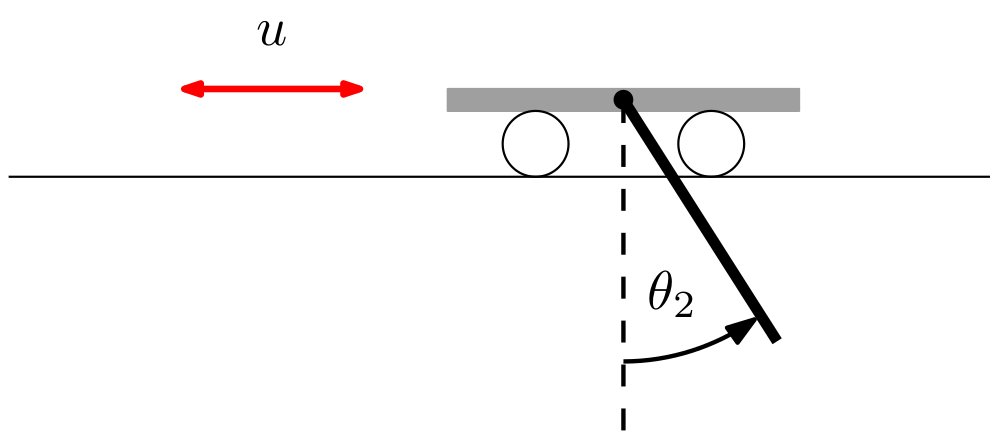
\includegraphics[width=0.5\textwidth]{Chapter3/Figures/cart-pole.png}
\caption[Cart-pole PILCO environment]{Cart-pole swing up. Source \cite{deisenroth2013pilco-documentation}.}
\label{Fig:cartpole-environment}
\end{figure}
The system has 4 continuous state variables: the position of the cart $x$, the velocity of the cart $\dot x$, the the pendulum angle $\theta_2$ and the angular velocity of the pendulum $\dot \theta_2$ of the pendulum. There is a target associated with each state variable.

\subsubsection{Pendubot}
The Pendubot shown in Fig. \ref{Fig:pendubot-environment}  is the second most complex environment used for experimentation. It consists of a central and outer pendulum of masses $m_1$ and $m_2$ and lengths $l_1$ and $l_2$, respectively. The two pendulums are linked together as well as the central pendulum being linked to the ground. The central and outer pendulum angles are given by $\theta_2$ and $\theta_3$, respectively, are measured anticlockwise from the upright vertical position. The link between the ground and the first pendulum can be actuated by the agent by applying a torque $u$ to the joint. The link between the pendulums cannot be actuated making the robot under actuated. The objective of the system is to actuate the central joint in such a way as to swing both pendulums to the upright vertical position and balanced there.
\begin{figure}[H]
\centering    
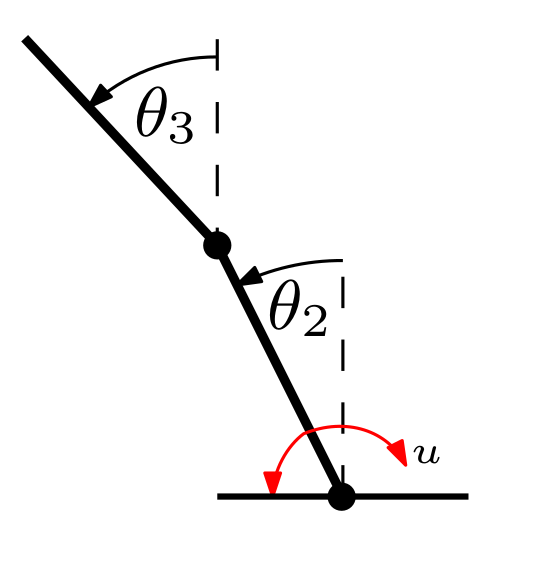
\includegraphics[width=0.25\textwidth]{Chapter3/Figures/pendubot.png}
\caption[Pendubot PILCO environment]{Source \cite{deisenroth2013pilco-documentation}.}
\label{Fig:pendubot-environment}
\end{figure}
The system has 4 continuous state variables: the angles of the pendulums $\theta_2$ and $theta_3$ and the angular velocities of the pendulums $\dot \theta_2$ and $\dot \theta_3$. There is a target associated with each state variable.

\subsubsection{Cart-Double-Pendulum}
The cart-double-pendulum shown in Fig. \ref{Fig:cartDoublePendulum-environment} is the most complex environment used for experimentation. It consists of a cart of mass $m_1$ and a central and outer pendulum of masses $m_2$ and $m_3$ and lengths $l_2$ and $l_3$, respectively. The two pendulums are linked together as well as the central pendulum being linked to the cart.  The central and outer pendulum angles are given by $\theta_2$ and $\theta_3$, respectively, and are measured anticlockwise from the upright vertical position. Continuous control actions $u$ applied to the cart cause it to move horizontally in the $x$-direction. The objective of the task is to actuate the cart in such a way that the double pendulum system is swung to the upright vertical position and balanced there while positioning the cart in the centre of the system at $x=0$. The unconstrained double pendulum system exhibits rich dynamical behaviour and is a chaotic system.
\begin{figure}[H]
\centering    
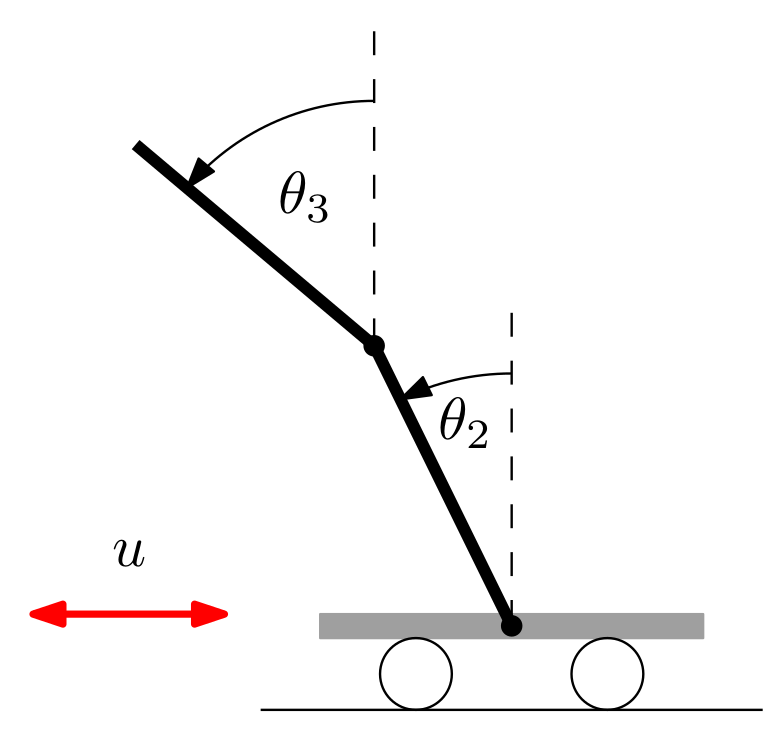
\includegraphics[width=0.3\textwidth]{Chapter3/Figures/cart-double-pendulum.png}
\caption[Cart-double-pendulum PILCO environment]{Source \cite{deisenroth2013pilco-documentation}.}
\label{Fig:cartDoublePendulum-environment}
\end{figure}
The system has 6 continuous state variables: the position of the cart $x$, the velocity of the cart $\dot x$, the angles of the pendulums $\theta_2$ and $theta_3$ the angular velocities of the pendulums $\dot \theta_2$ and $\dot \theta_3$. There is a target associated with each state variable.


\section{Experimental Results}

\subsection{The Evolution of Distributions over States and Costs}
The Monte-Carlo uncertainty estimates are performed by rolling out state-action values through the dynamics model using the one-step predictions in Eq. \ref{Eq:model-posterior-one-step} and for each state visited a cost is calculated with Eq. \ref{Eq:PILCO-cost-function} . PILCO's direct policy search method is formulated so that the cost is directly consulted when deciding a policy (see Eq \ref{Eq:PILCO-expected-return}) and not the state itself (although the cost is a function of the state). It is therefore important illustrate the difference by observing how the distribution over states and the distribution over costs evolve as they are propagated through the model in the context of the Monte-Carlo method presented in Section \ref{S:monte-carlo-estimate}.

This is demonstrated by performing $9$ steps through the simple $1$\textit{-dimensional} transition function shown in Fig. \ref{Fig:1-dimensional-transition-function}. The transition function represents the input space $\mathbf{x}_{t}\in [-5, 5]$ and is trained on targets representing the next state $\mathbf{x}_{t+1}$, not state differences as is done with PILCO. Fig. \ref{Fig:1-dimensional-transition-function} shows the trigonometric basis function model's predictive mean and $95\%$ confidence interval over observed state transitions and $4$ functions drawn from the posterior distribution over the model weights $q(\mathbf{w})$. To illustrate the evolution of state and cost distributions for the first step through the transition function, $M=1000$ sets of weights $\mathbf{w} \sim q(\mathbf{w})$ were sampled and for each set, $N=1000$ starting states drawn from $\mathbf{x}_{0} \sim \mathcal{U}(-5,5)$ were stepped through the function according to Eq. \ref{Eq:model-posterior-one-step}. This process was repeated $8$ more times but for each step, the next state $\mathbf{x}_{t+1}$ as predicted by Eq. \ref{Eq:model-posterior-one-step} was fed back into the equation as the input state $\mathbf{x}_{t}$. At each step the cost was calculated with Eq. \ref{Eq:PILCO-cost-function} with width $\sigma_{c}=1.5$ and target state $\mathbf{x}_{\text{target}}=0$. There is no explicit policy used here. This can be viewed as if there is only one action and the agent selects that action at each opportunity. This enables the states and costs to evolve freely under the system dynamics.

\begin{figure}[htp!]
\centering    
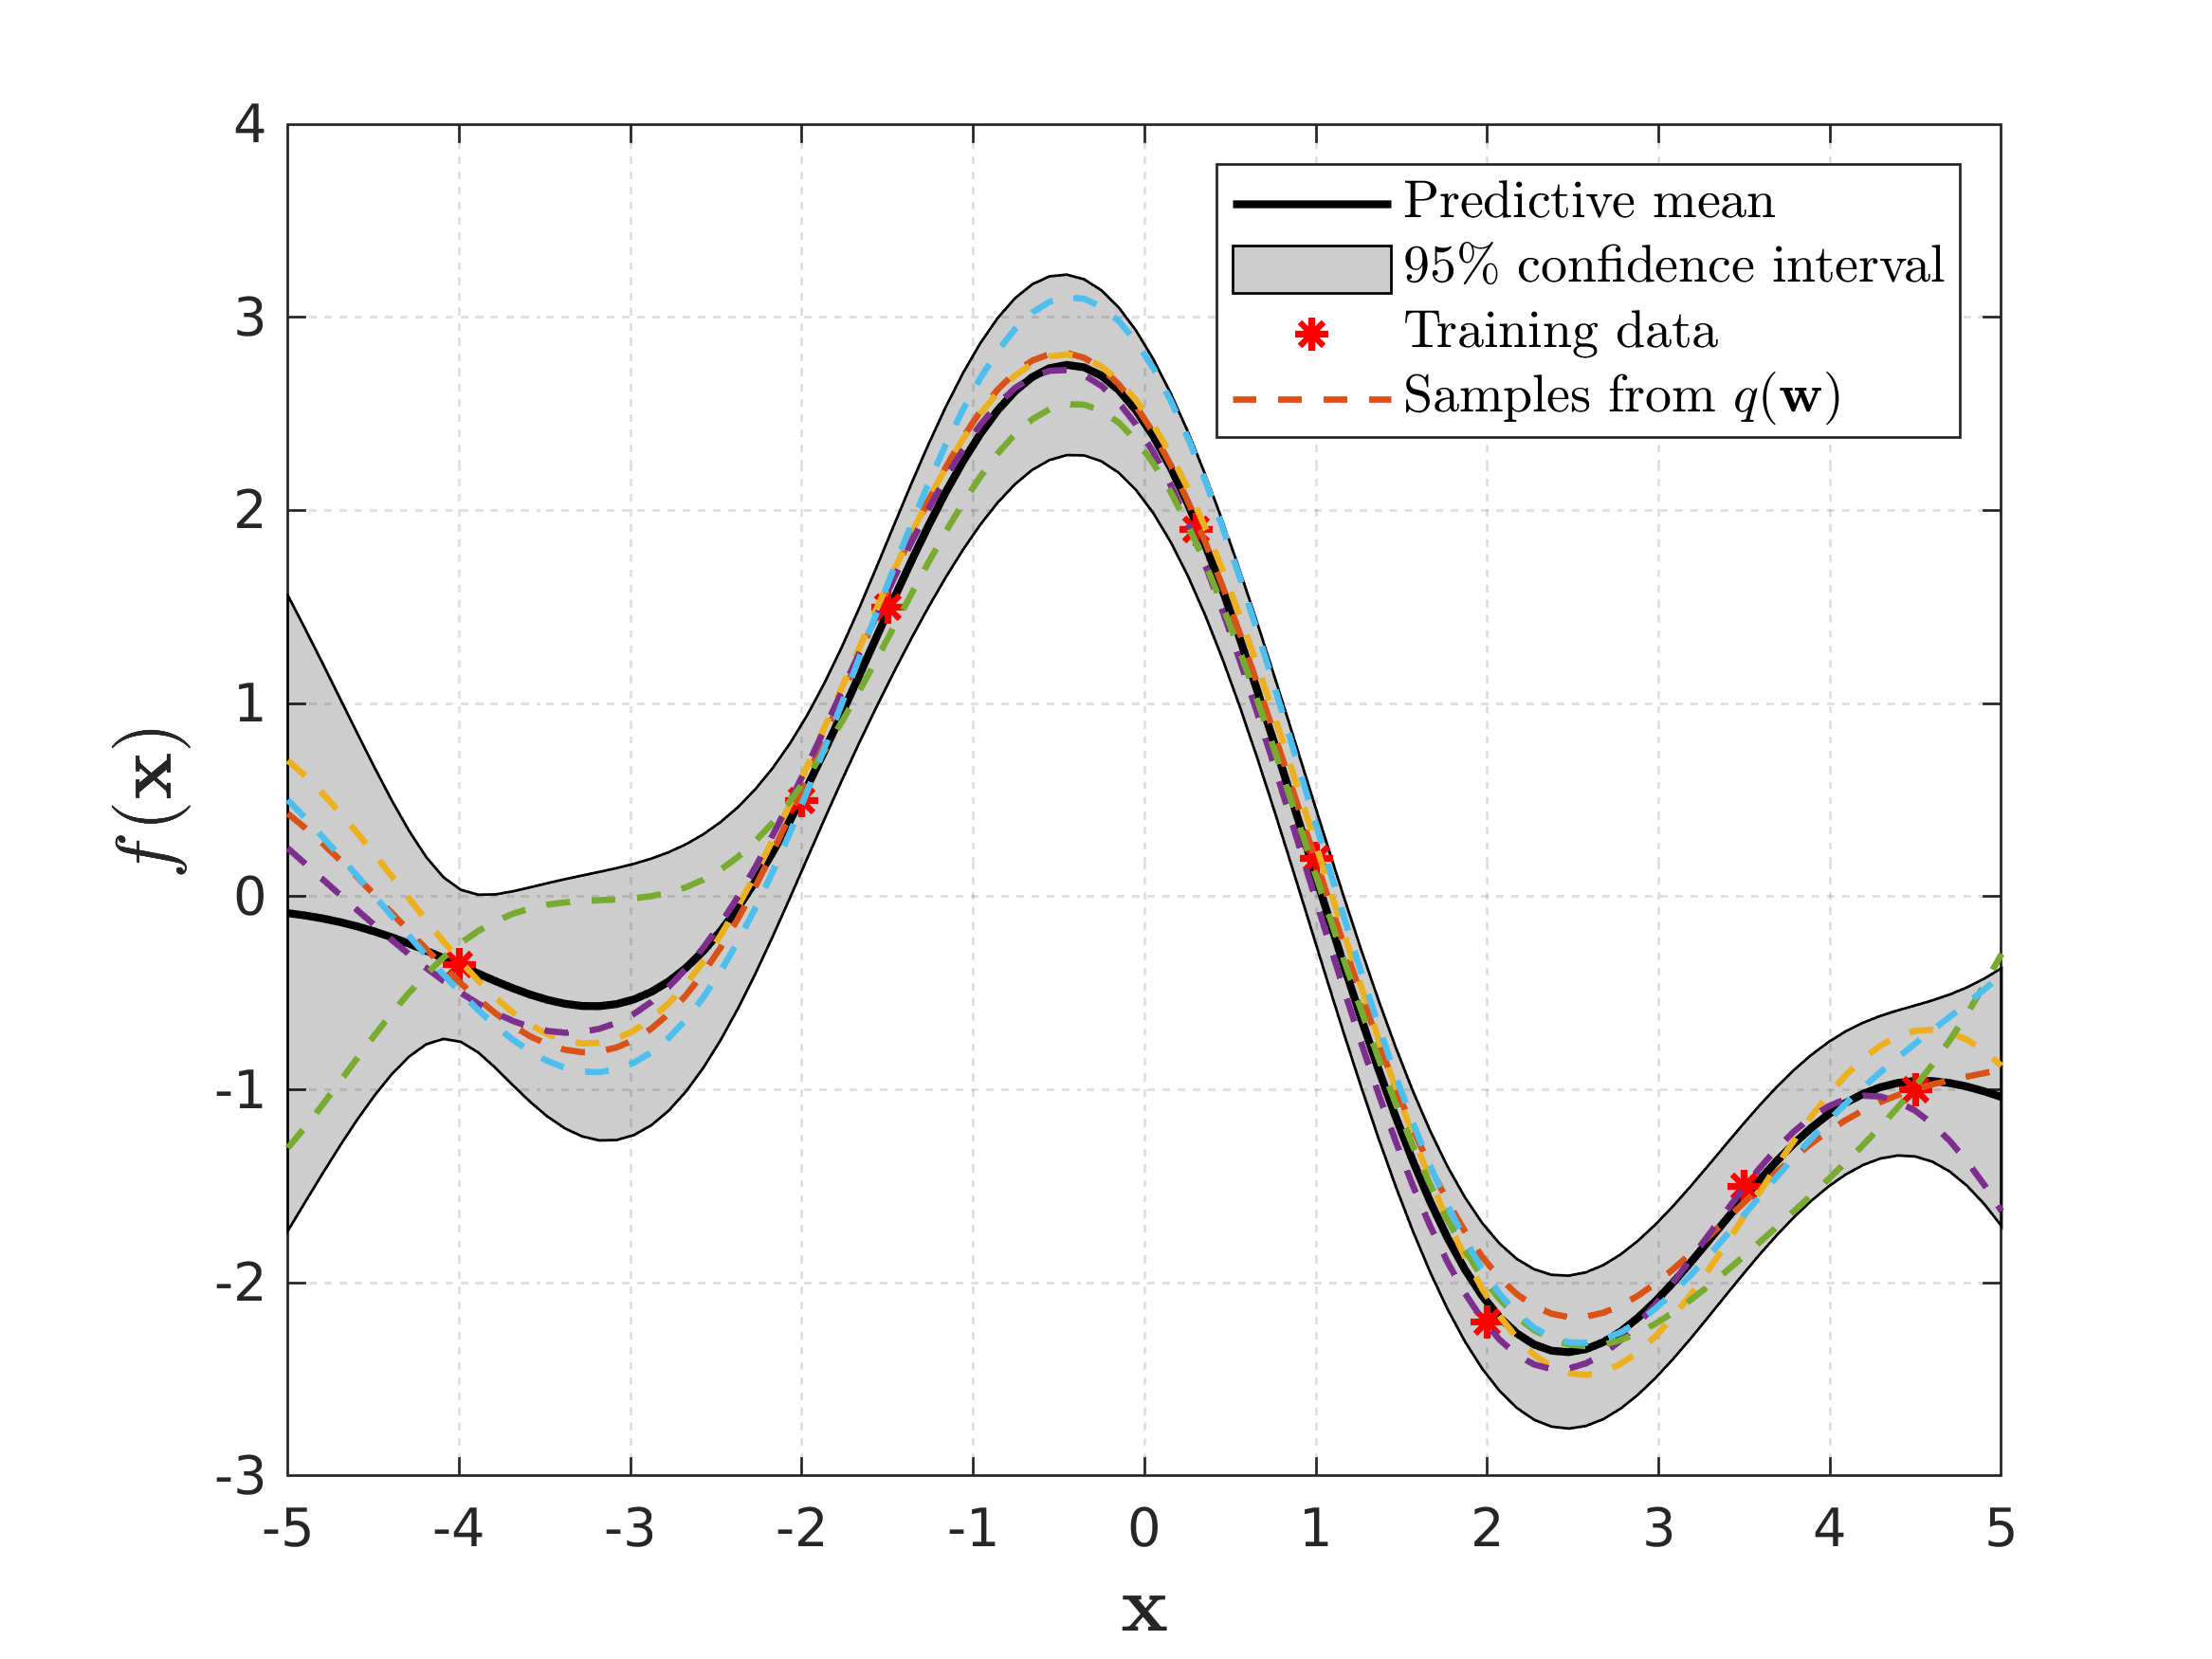
\includegraphics[width=0.6\textwidth]{Chapter3/Figures/transition_function.png}
\caption[A 1-dimensional transition function example]{A 1-dimensional transition function example}
\label{Fig:1-dimensional-transition-function}
\end{figure}

Fig \ref{Fig:Re-evolution-of-state-and-cost} shows the evolution of the distributions over states and costs for input distributions (\ref{Fig:Re-hist-traj-1} and \ref{Fig:Re-hist-cost-1}), after 1 transition (\ref{Fig:Re-hist-traj-2} and \ref{Fig:Re-hist-cost-2}) and 9 transitions (\ref{Fig:Re-hist-traj-4} and \ref{Fig:Re-hist-cost-4}). The distribution over costs associated with the uniform initial distribution over states reveals the locally quadratic nature of the cost function where the high density at $\mathbb{C}(x)=1$ indicates saturation of costs associated with states further away from the target state. After the first step, the distribution over states tightens around the target state with a peak about $\mathbf{x}=-0.7$. The reduction in the state distribution tails means that the cost no longer saturates and the tightening around the target state has increased the cost density about $\mathbb{C}(\mathbf{x})=0$. Finally, after 9 steps, the state distribution flattens out with small peaks around the $\pm\mathbf{x}=2$. The high density about $\mathbb{C}(x)=0$ reduces and a bump forms about the $\mathbb{C}(x)=0.8$ position corresponding to the peaks of the state distribution at $\pm\mathbf{x}=2$. 
\begin{figure}[htp!]    
\begin{subfigure}[b]{0.48\linewidth}
    \centering
    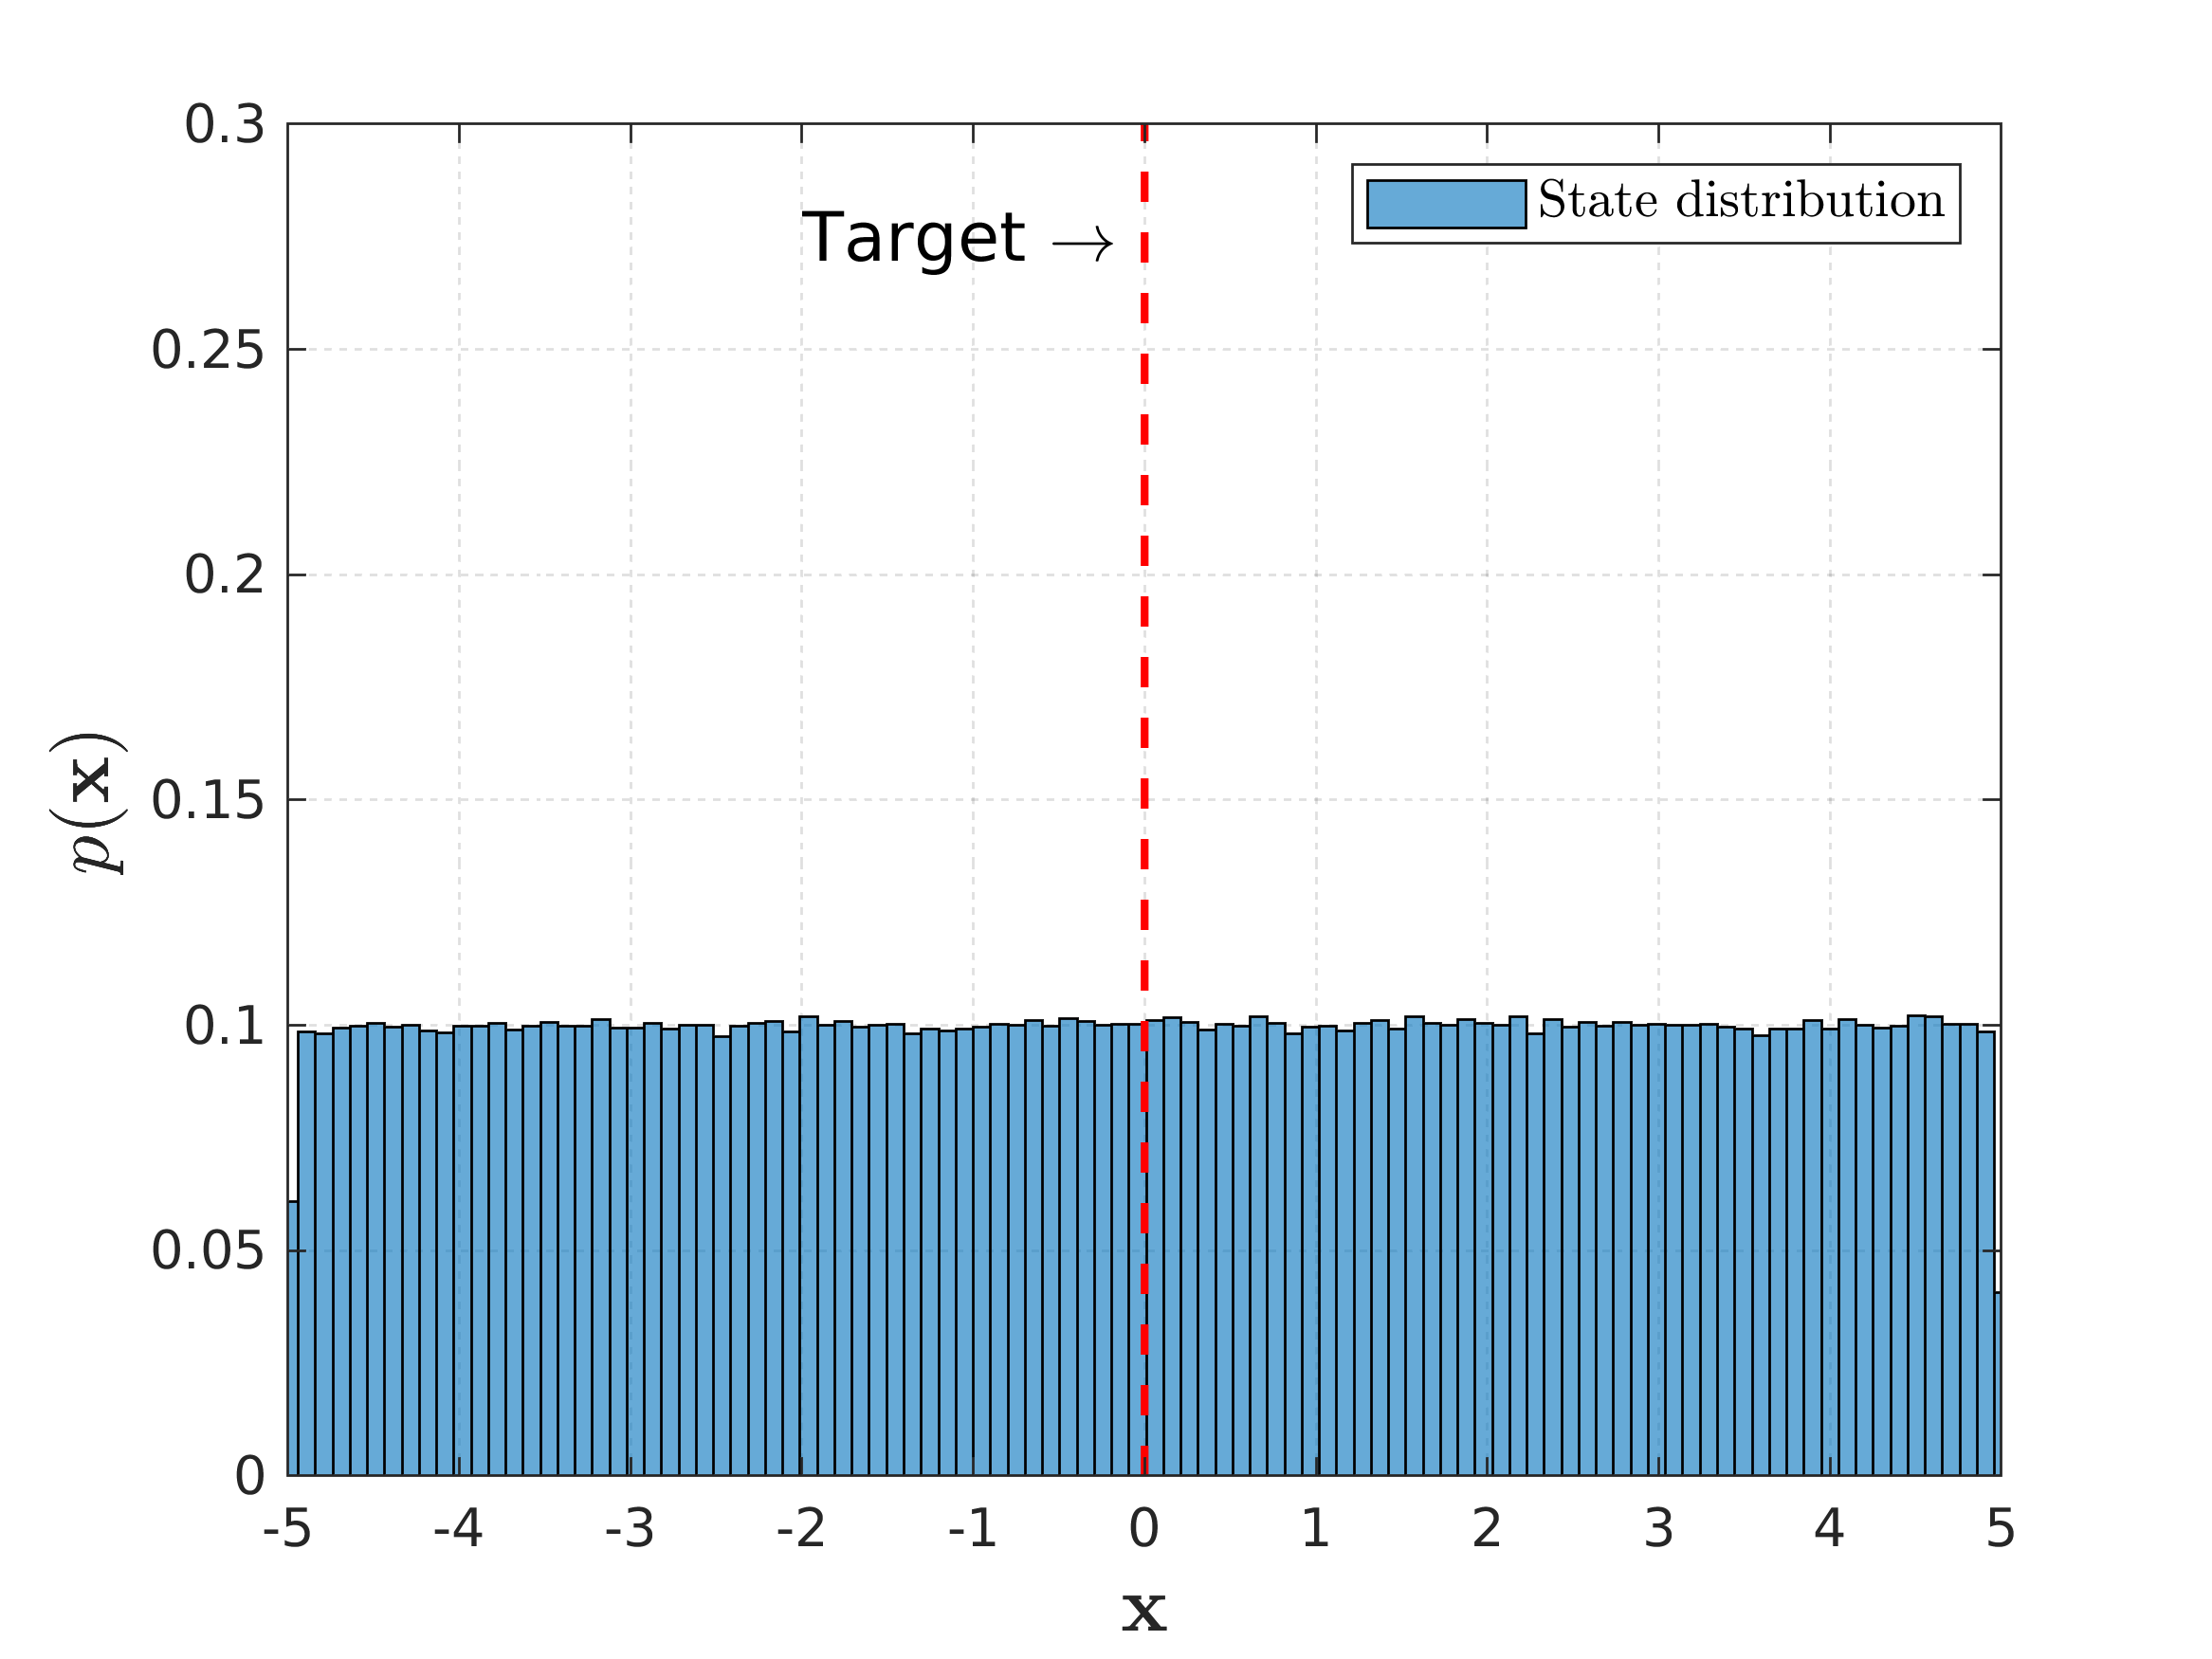
\includegraphics[height=0.22\textheight,width=0.95\textwidth]{Chapter3/Figures/trans_traj_hist_1.png} 
    \caption{Input distribution over states} 
    \label{Fig:Re-hist-traj-1} 
  \end{subfigure} 
  \hspace{\fill}  %% maximize space between adjacent subfigures
  \begin{subfigure}[b]{0.48\linewidth}
    \centering
    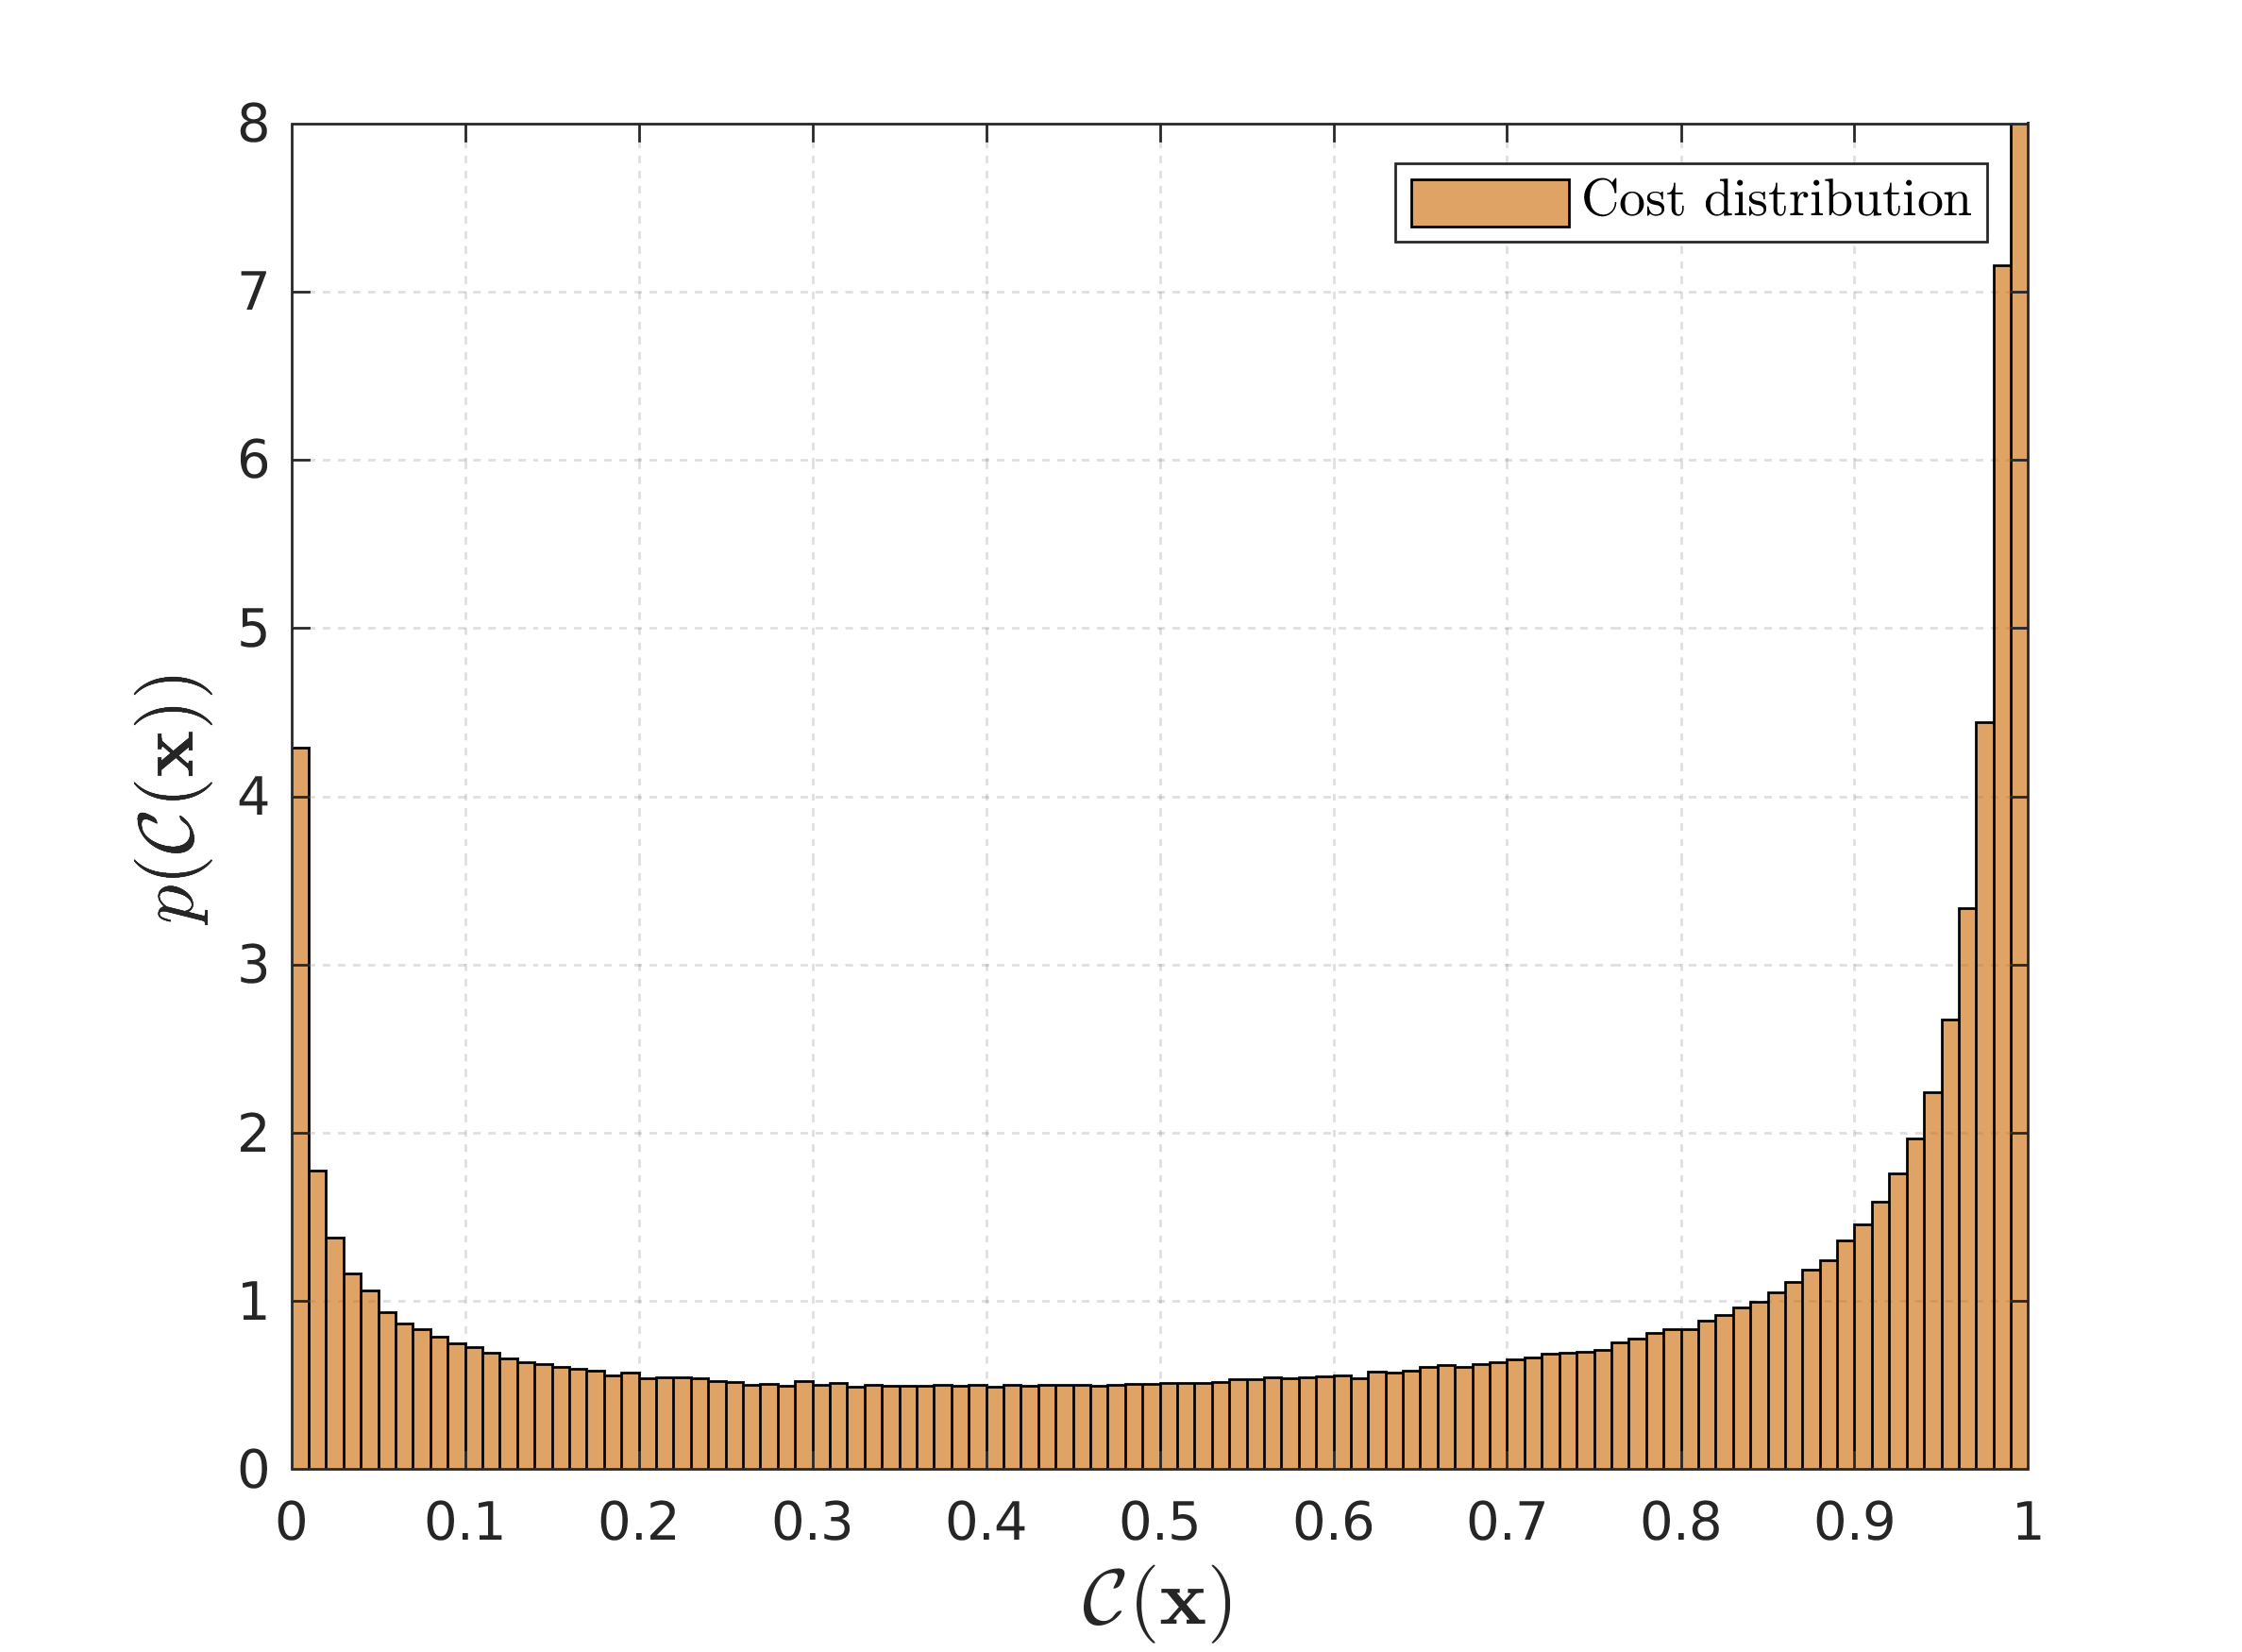
\includegraphics[height=0.22\textheight,width=0.95\textwidth]{Chapter3/Figures/trans_cost_hist_1.png} 
    \caption{Input distribution over costs} 
    \label{Fig:Re-hist-cost-1} 
  \end{subfigure} 

  \vspace{4ex}  %% extra vertical space
  \begin{subfigure}[b]{0.48\linewidth}
    \centering
    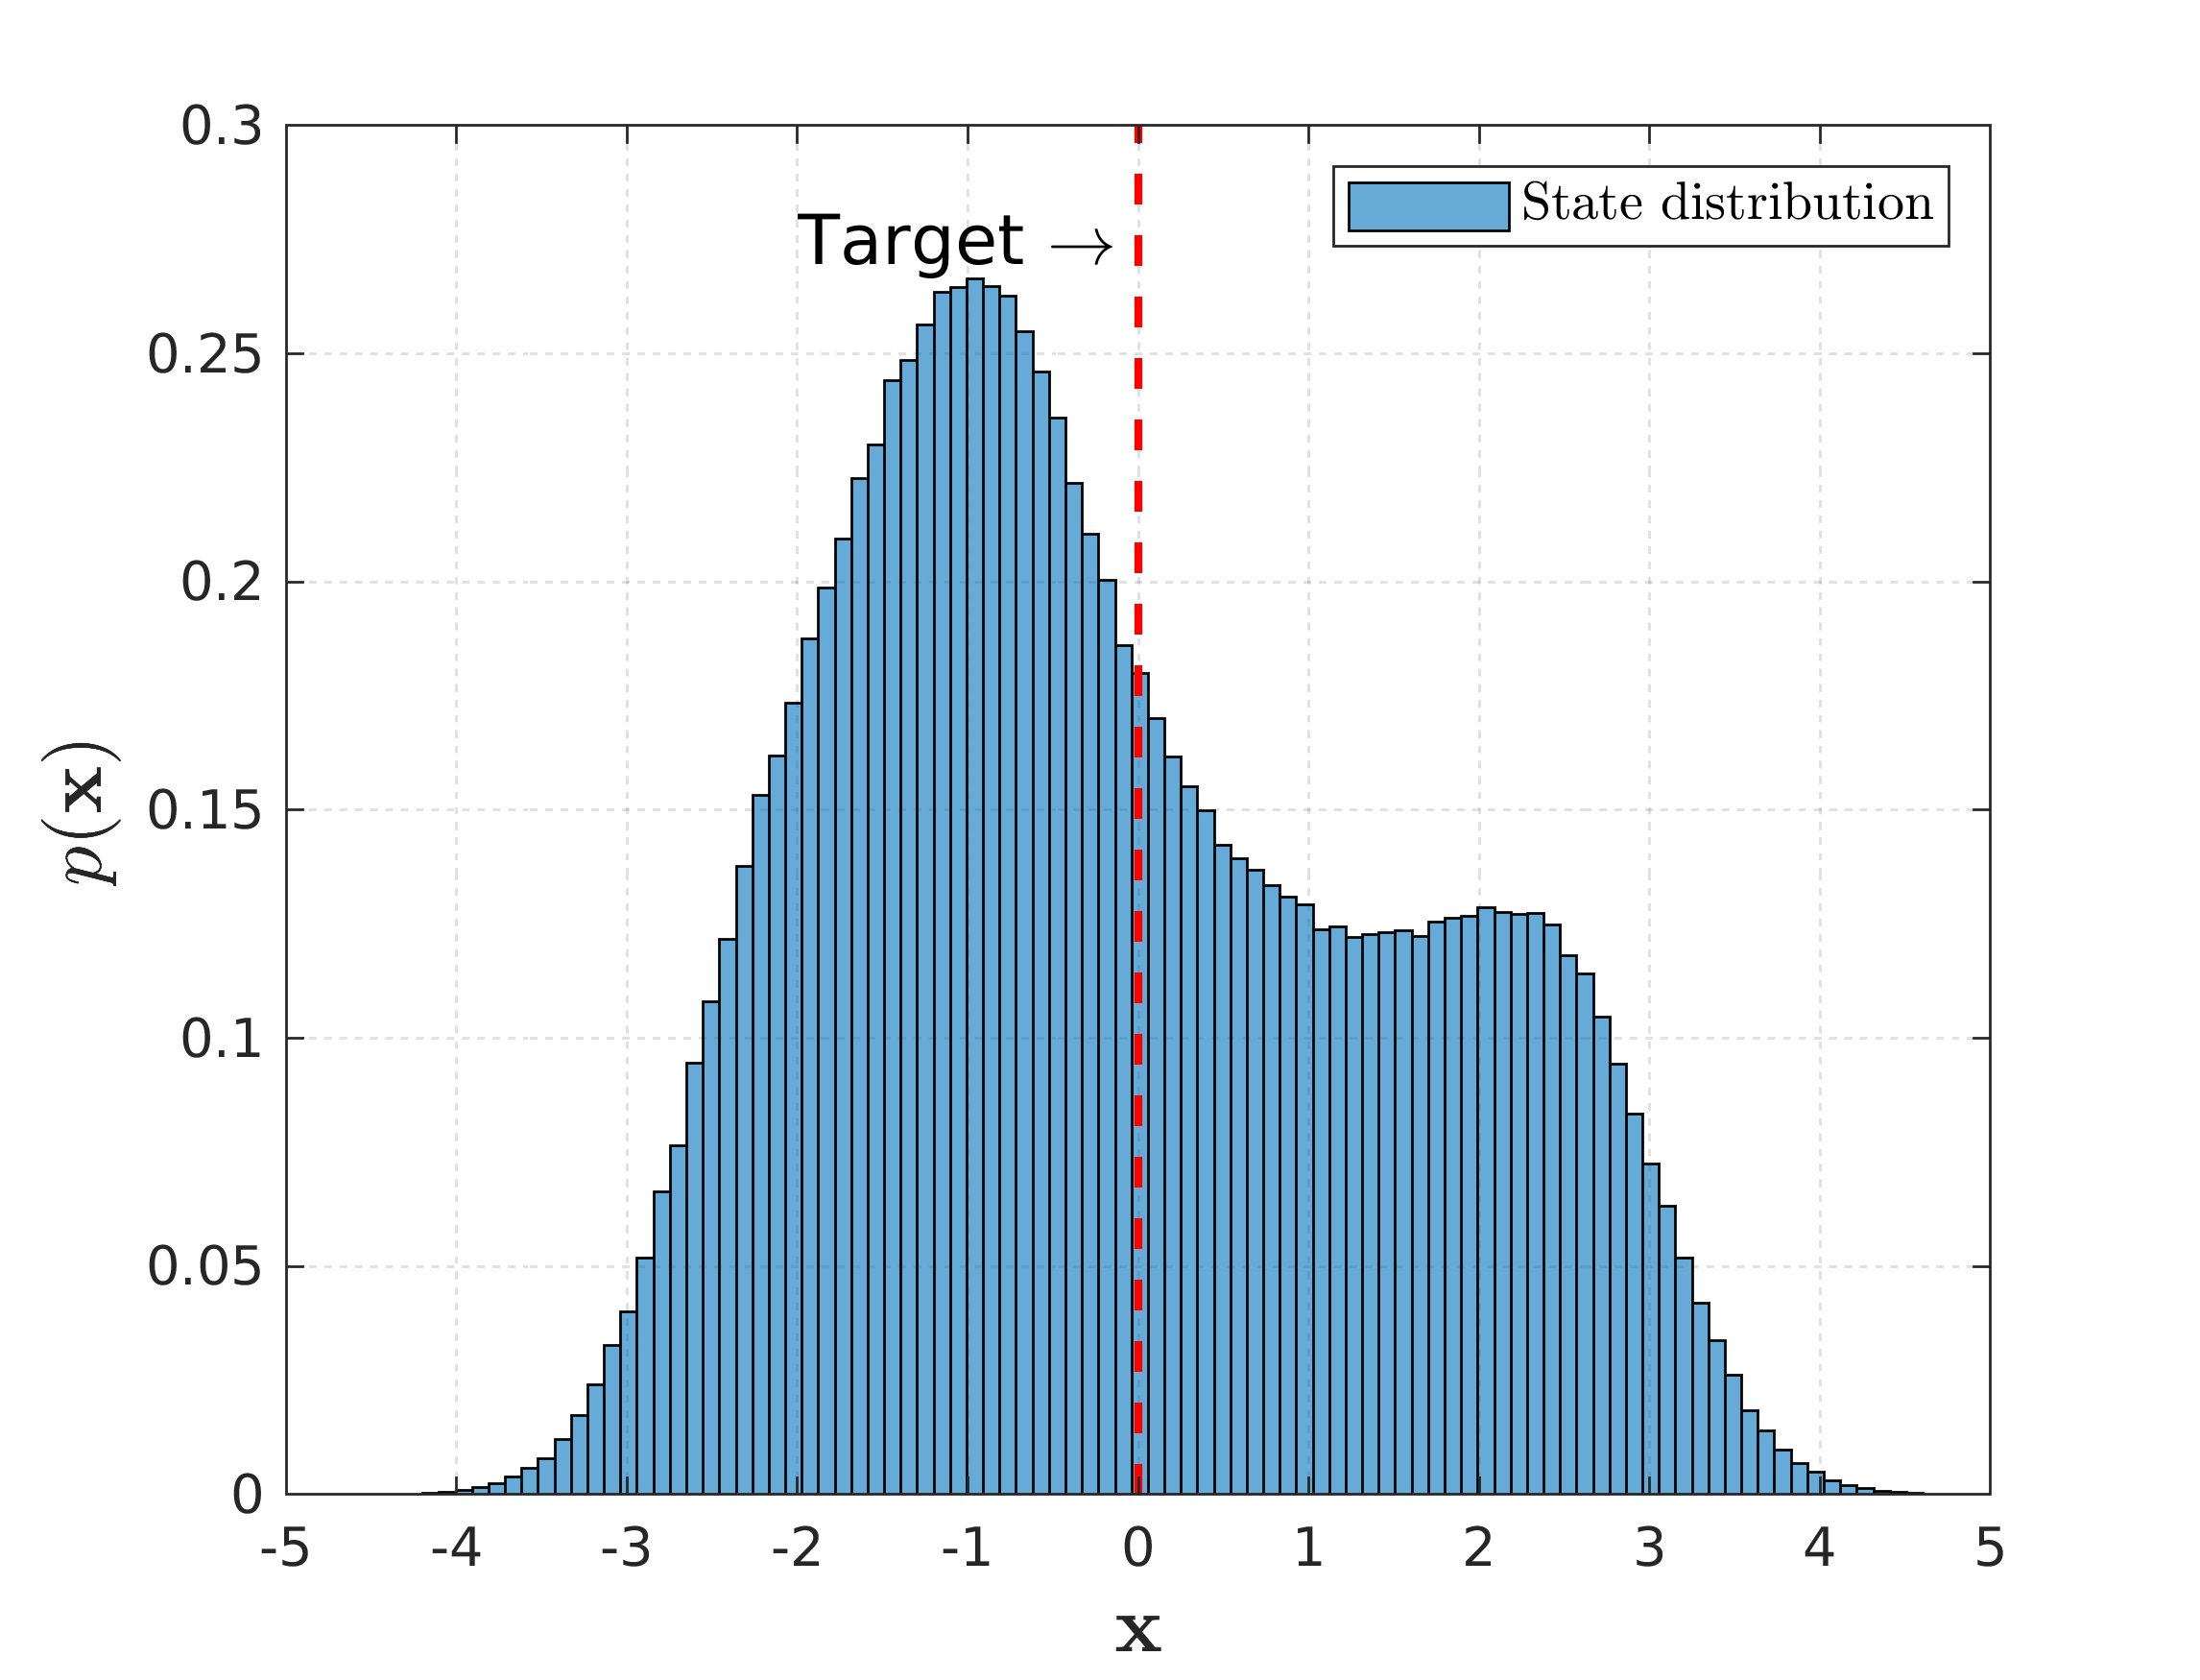
\includegraphics[height=0.22\textheight,width=0.95\textwidth]{Chapter3/Figures/trans_traj_hist_2.png} 
    \caption{Distribution over states after 1 transition} 
    \label{Fig:Re-hist-traj-2} 
  \end{subfigure} 
  \hspace{\fill}
  \begin{subfigure}[b]{0.48\linewidth}
    \centering
    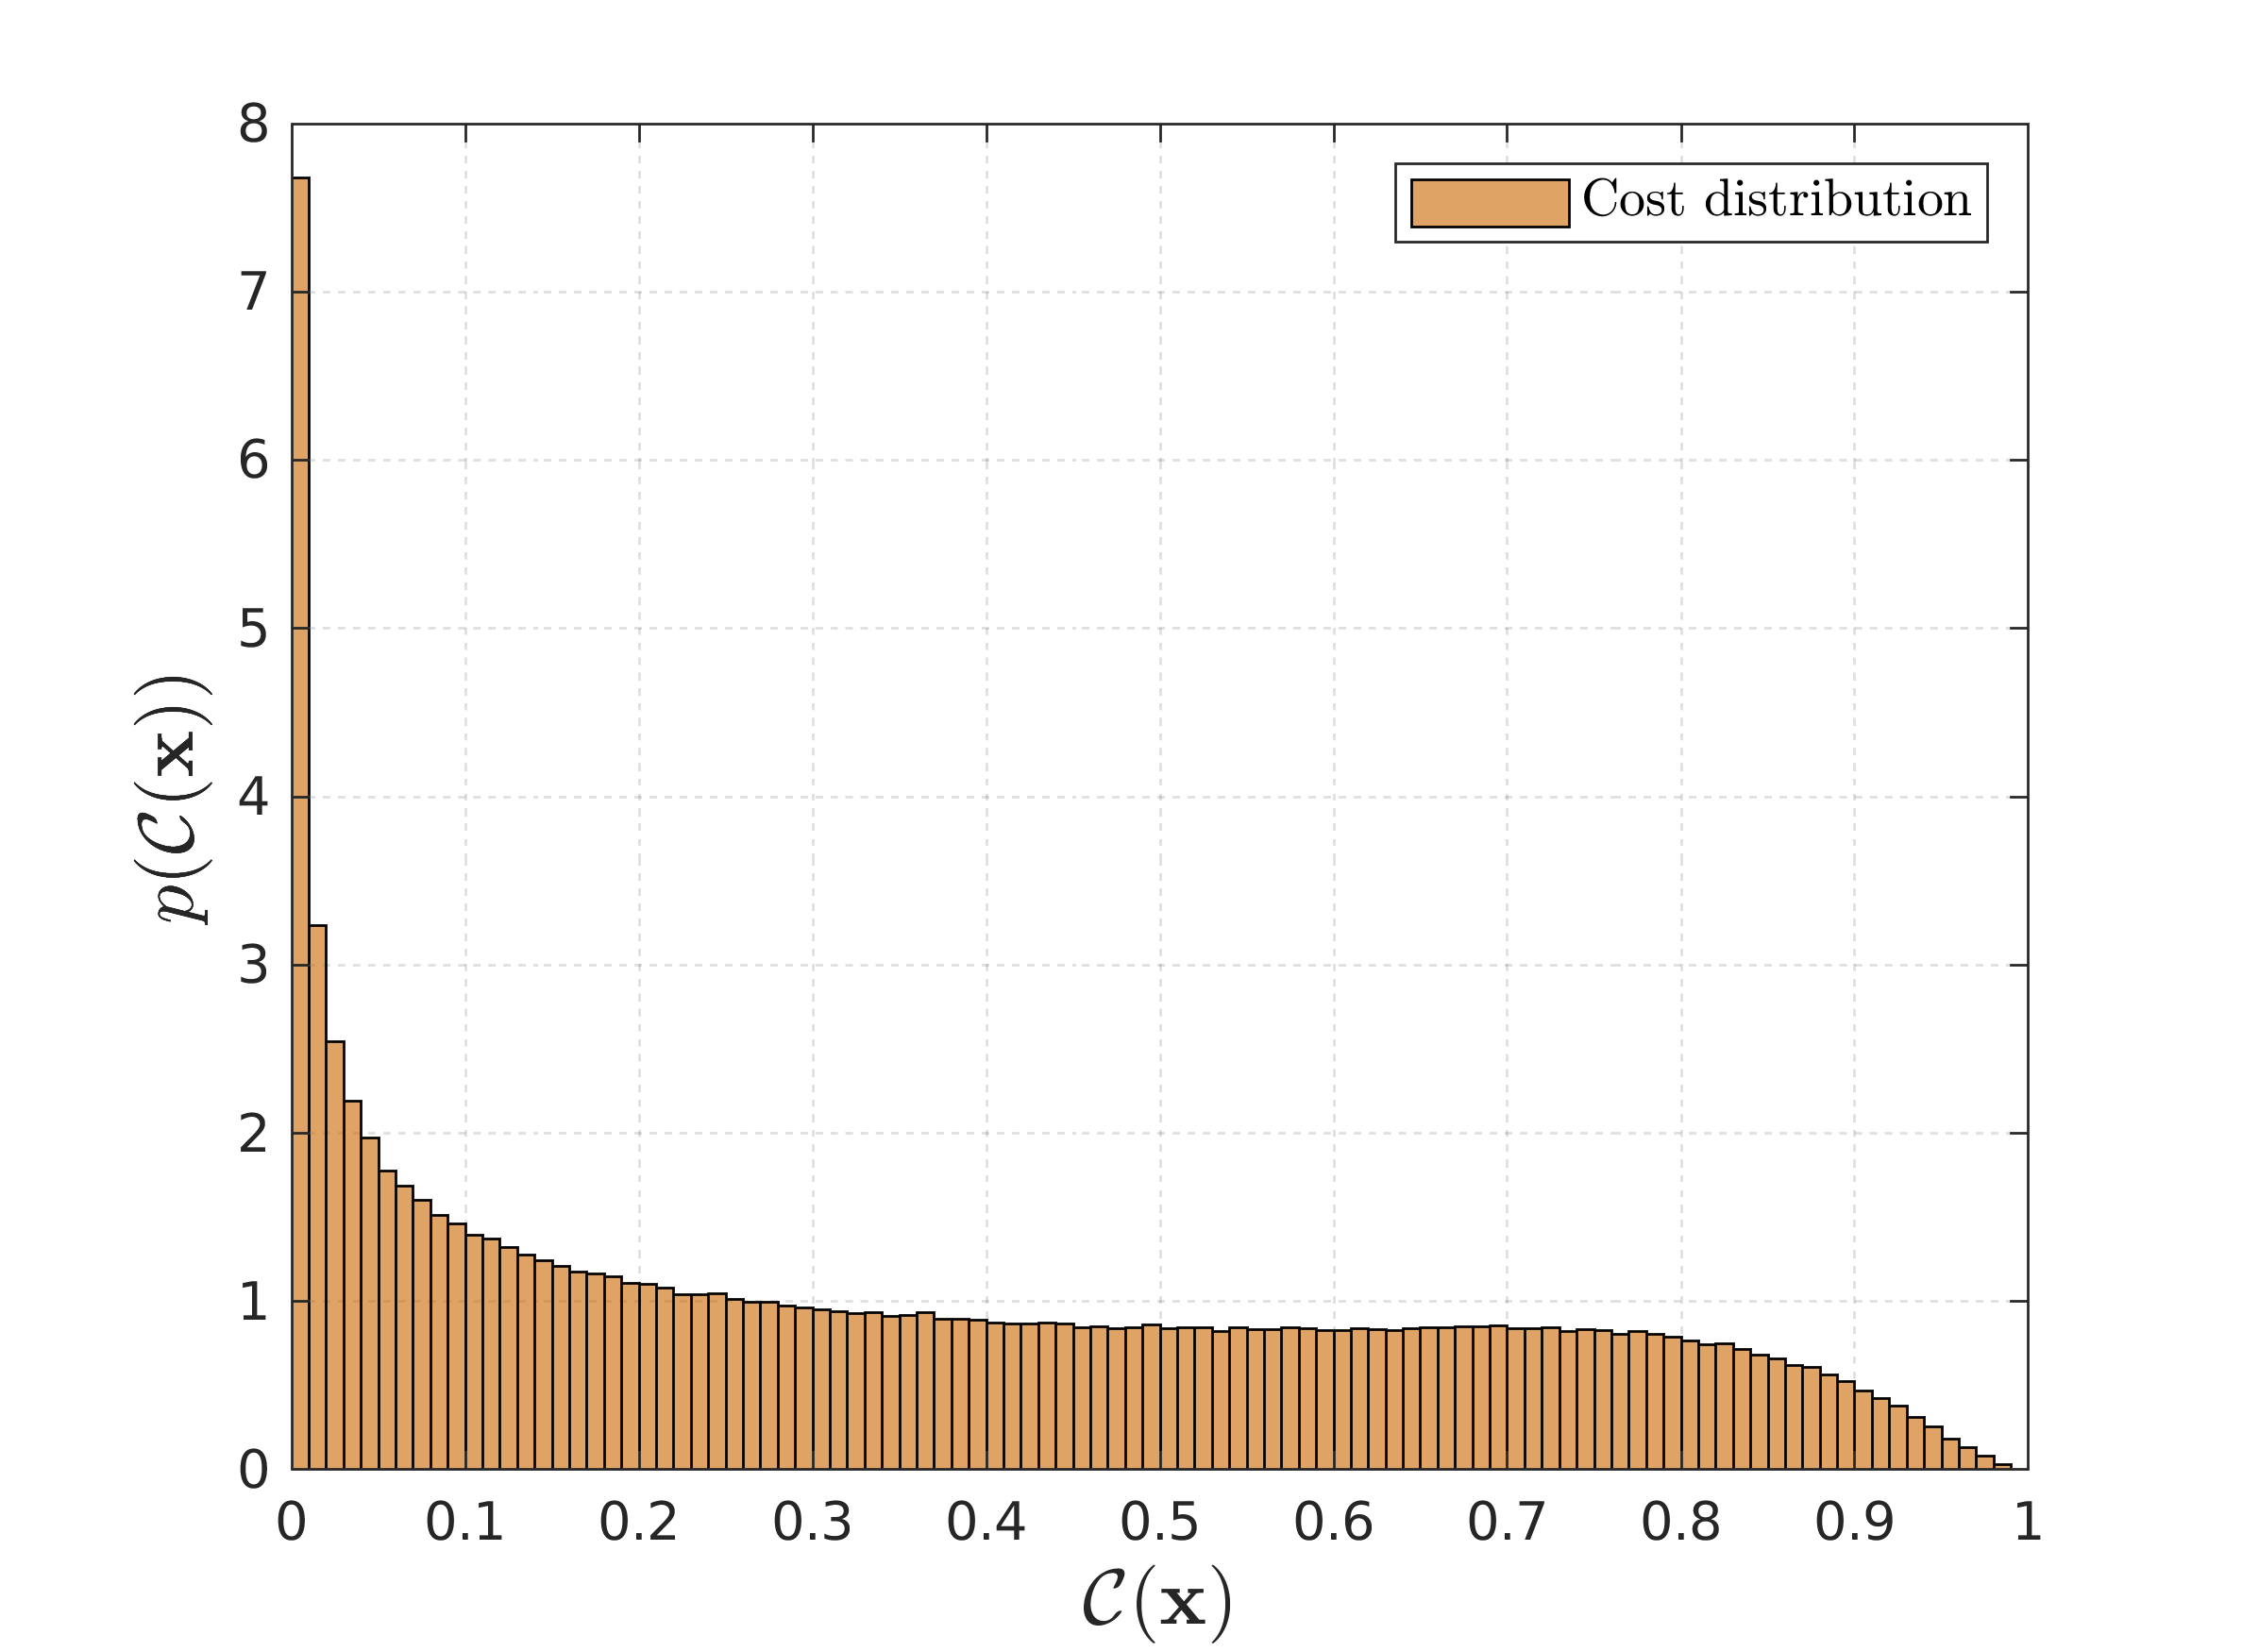
\includegraphics[height=0.22\textheight,width=0.95\textwidth]{Chapter3/Figures/trans_cost_hist_2.png} 
    \caption{Distribution over costs after 1 transition} 
    \label{Fig:Re-hist-cost-2} 
  \end{subfigure} 

    \vspace{4ex}
  \begin{subfigure}[b]{0.48\linewidth}
    \centering
    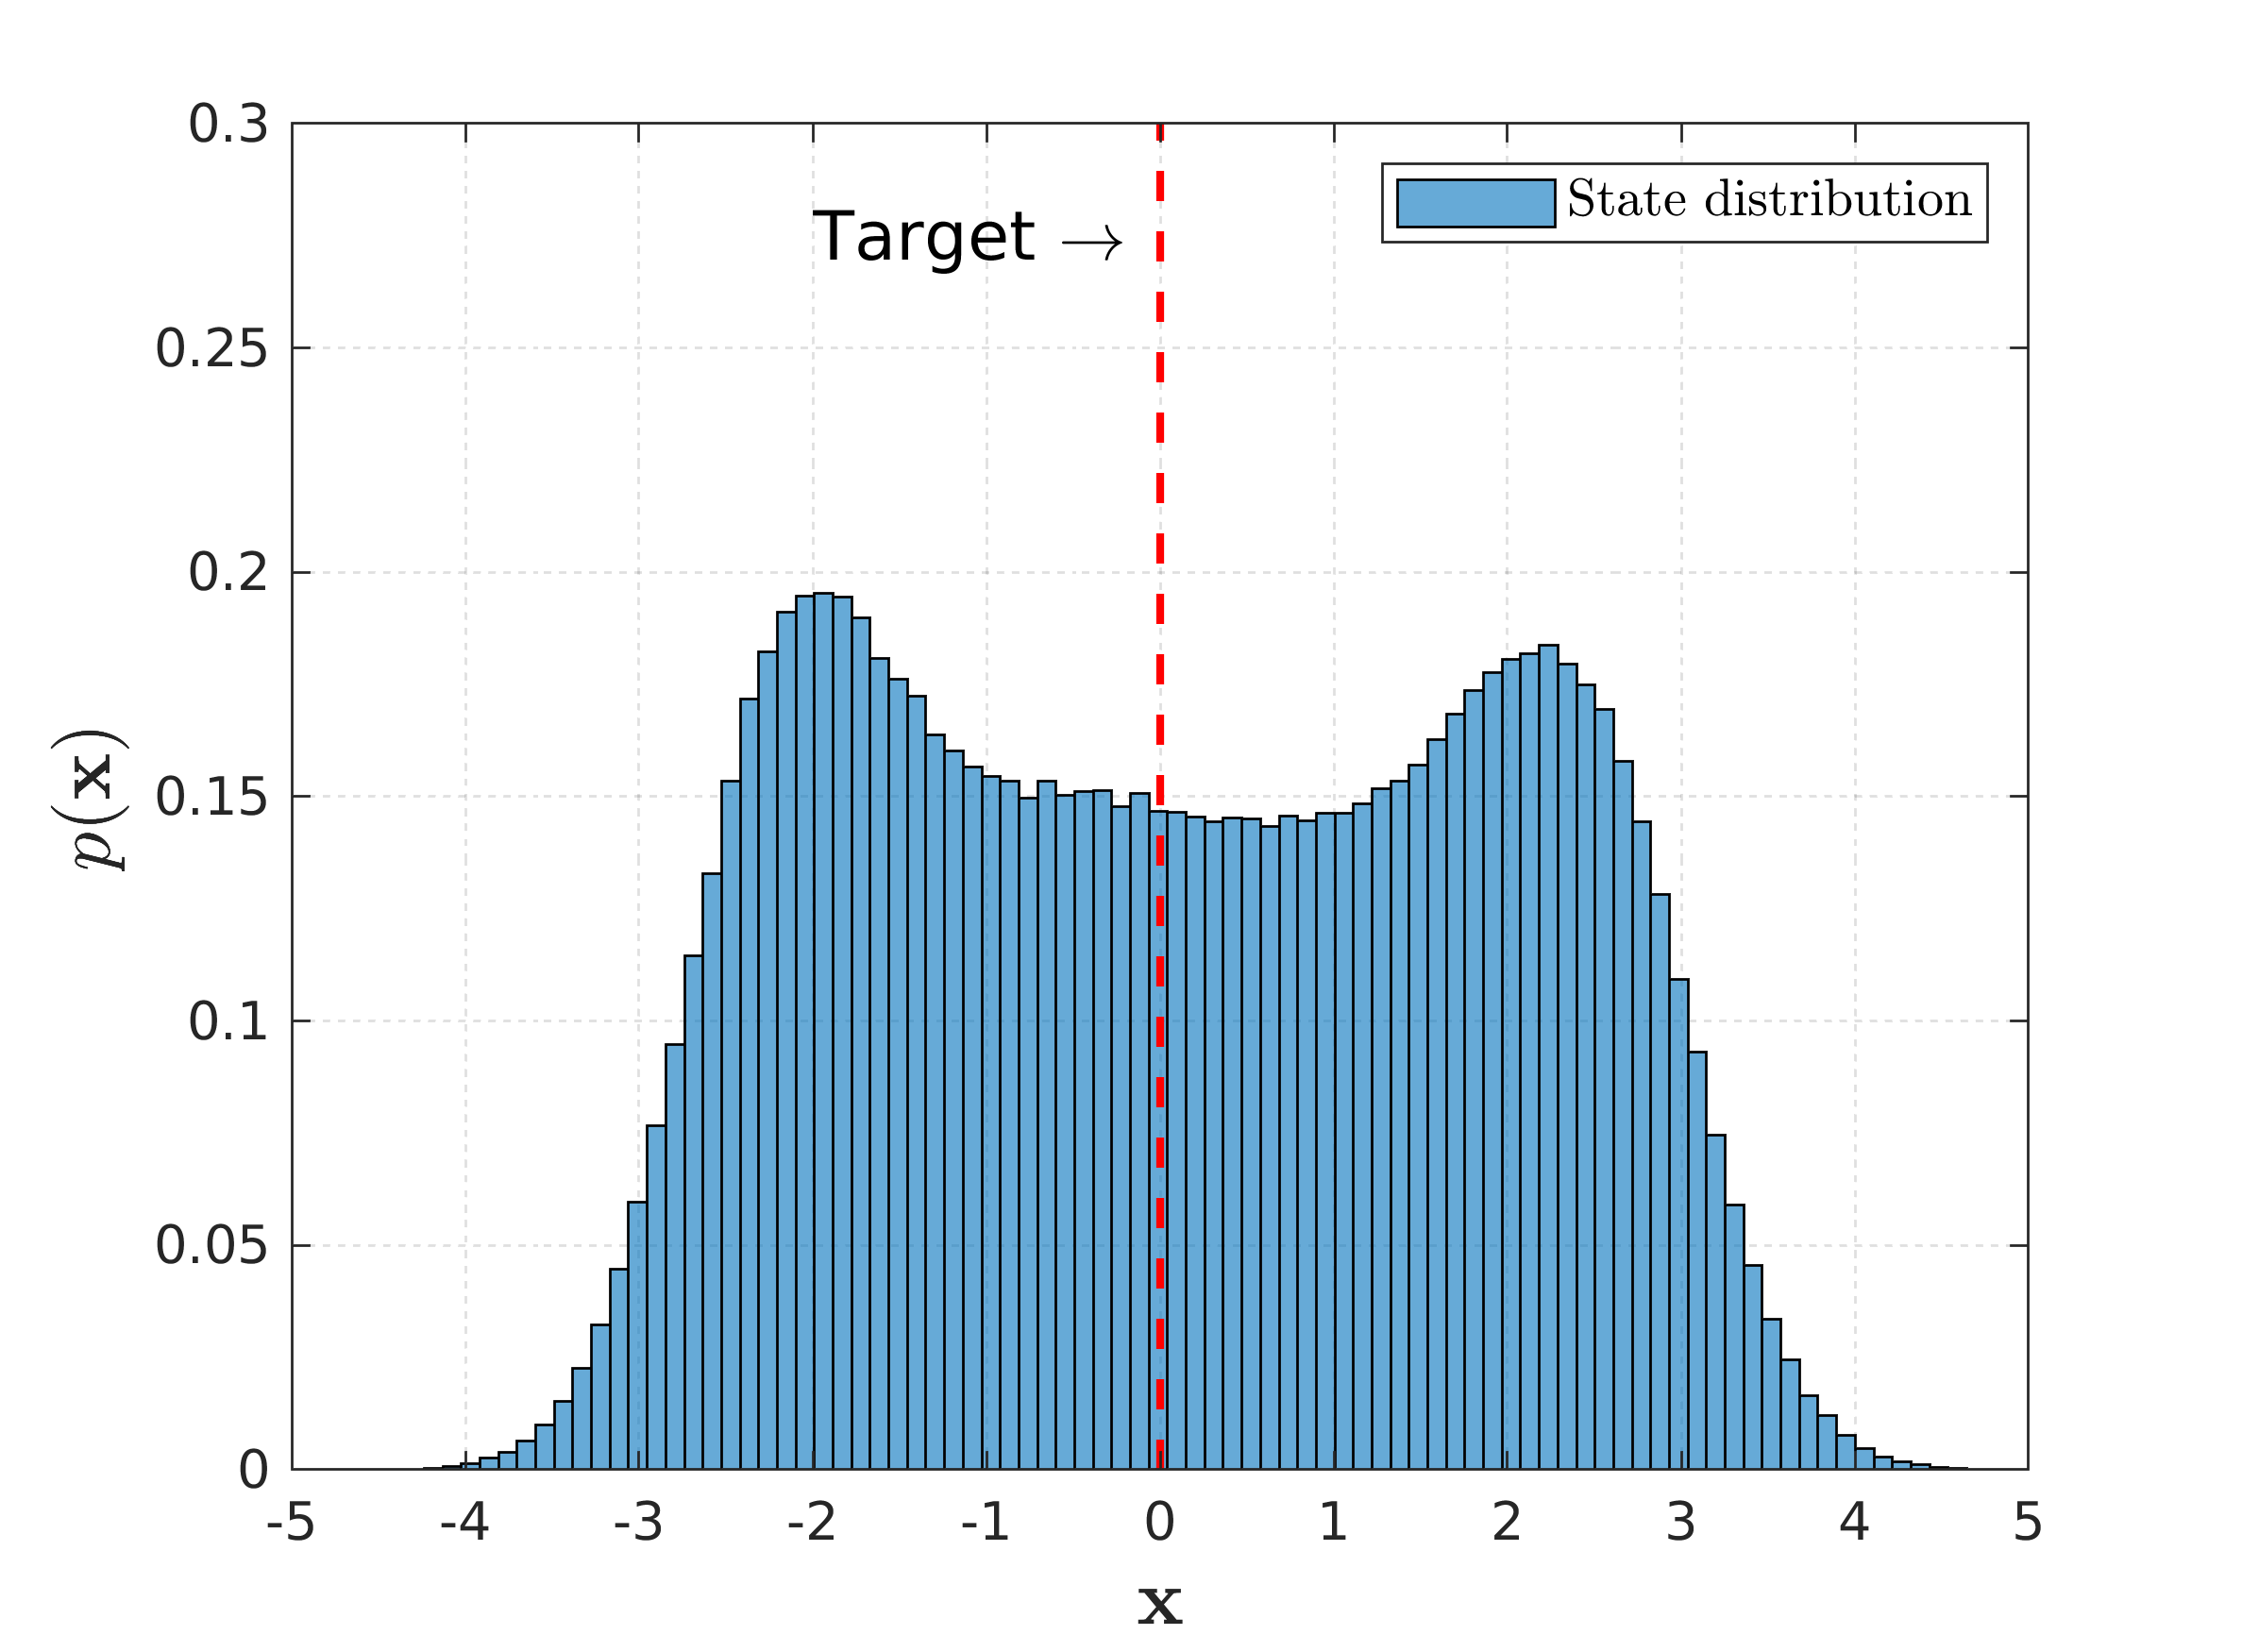
\includegraphics[height=0.22\textheight,width=0.95\textwidth]{Chapter3/Figures/trans_traj_hist_4.png} 
    \caption{Distribution over states after 9 transitions} 
    \label{Fig:Re-hist-traj-4} 
  \end{subfigure}
  \hspace{\fill}
  \begin{subfigure}[b]{0.48\linewidth}
    \centering
    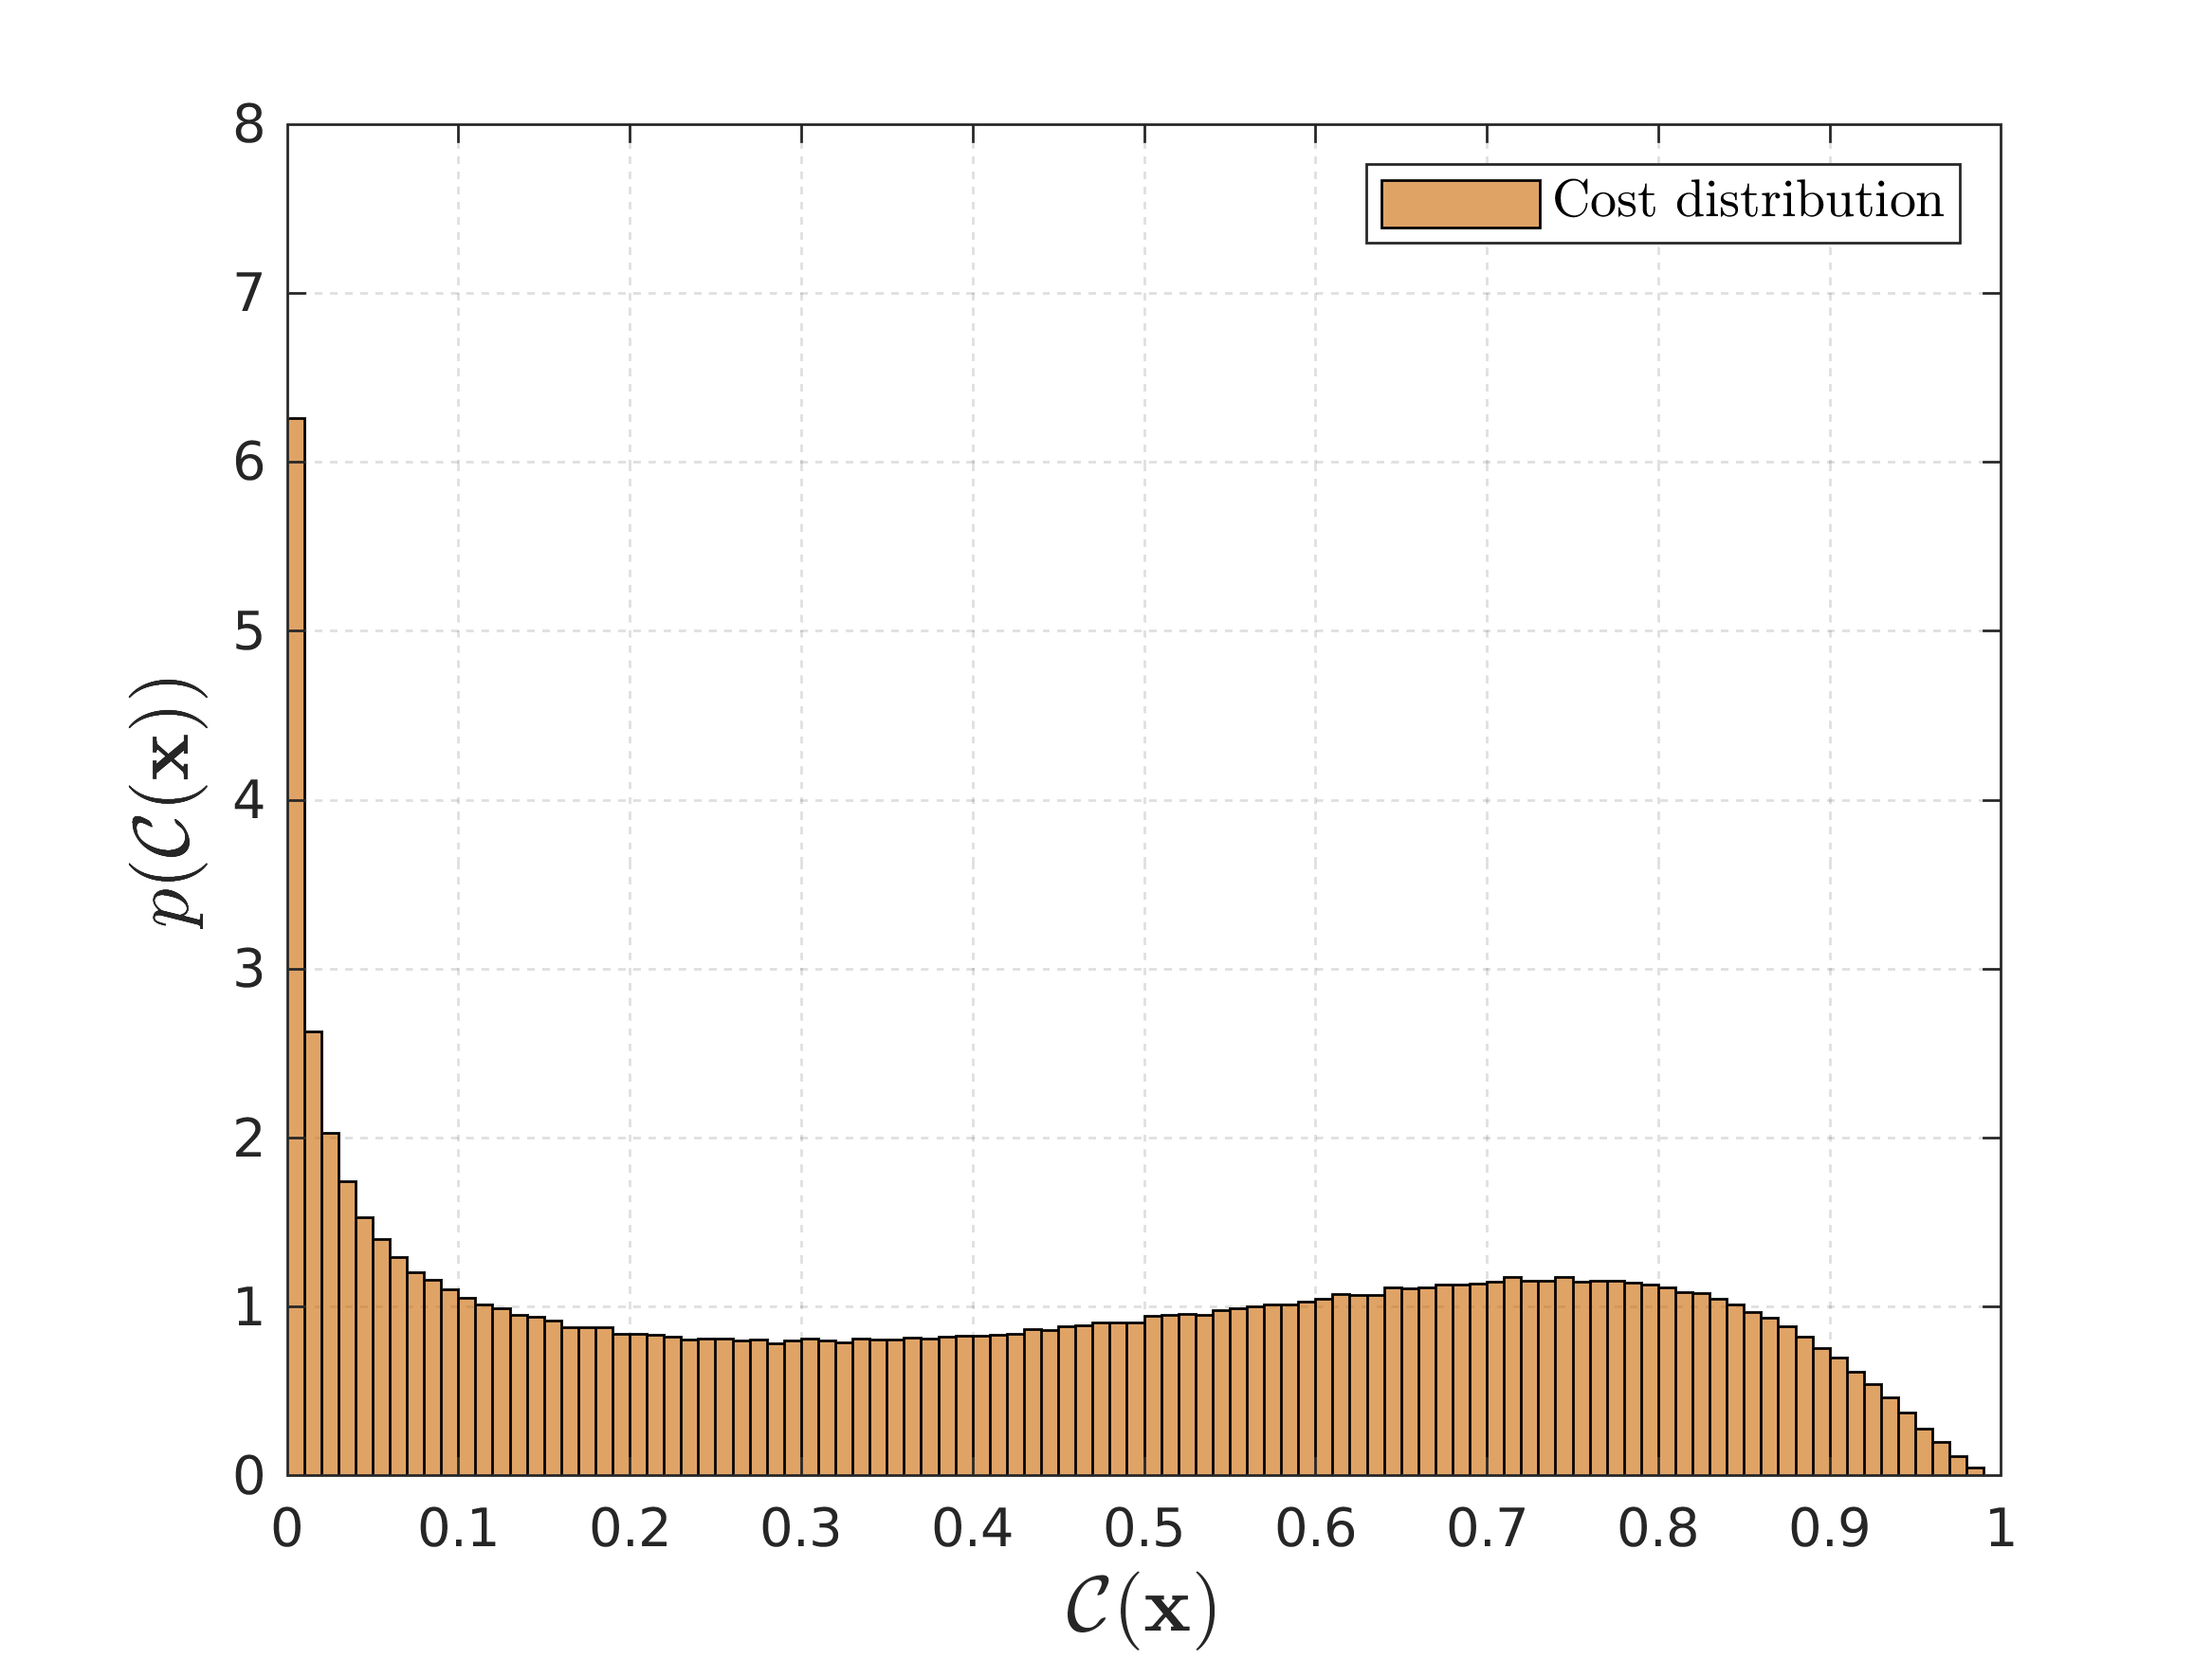
\includegraphics[height=0.22\textheight,width=0.95\textwidth]{Chapter3/Figures/trans_cost_hist_4.png} 
    \caption{Distribution over costs after 9 transitions} 
    \label{Fig:Re-hist-cost-4} 
  \end{subfigure} 
\caption[Evolution of state and cost distributions]{The evolution of state and cost distributions with increasing numbers of steps through the transition function.}
\label{Fig:Re-evolution-of-state-and-cost} 
\end{figure}

\subsection{A Decomposition of Transition Function Uncertainty}
A toy data set with target noise variance 0.0625 is used to illustrate the Monte-Carlo scheme for estimating the aleatoric and epistemic uncertainties present in the cost $\mathbb{C}(\mathbf{x})$ under policy $\pi$. Similar to the previous experiment, a 1-dimensional transition function is used and an explicit policy is not defined. This is viewed as if there is only one action available for selection and the agent selects that action at each opportunity and allows the system dynamics to evolve freely over time. In this experiment, the agent begins by observing 4 transition data points. It then progressively observes more data a single point at a time up to a total of 50 data points. At each observation, the trigonometric basis function model is used to form a belief over the transition dynamics of the environment. Fig. \ref{Fig:Re-pred-4-points}-\ref{Fig:Re-pred-50-points} shows the predictive distribution over the transition data and 4 functions sampled from the posterior distribution over the parameters after 4, 25 and 50 observations, respectively. For this, the lengthscale of the spectral points is purposely set to a large value to over fit the data as can be seen in Fig. \ref{Fig:Re-pred-4-points}. This is done for two reasons: to artificially induce more epistemic uncertainty into the model and to be more representative of a higher dimensional space where the observation of a single data point provides the model with more information than in the 1-dimensional case. The figures show that as more data is observed, the model becomes increasingly confident about the parameters. This can be seen in the functions drawn from the posterior distribution over the model parameters which increasingly resemble the predictive mean as confidence grows. 

Each time a new data point is observed, Monte-Carlo trajectory roll outs are performed through the model using the procedure described in Sec. \ref{S:monte-carlo-estimate} and the uncertainty is decomposed into its aleatoric and epistemic components using Eq. \ref{S:monte-carlo-estimate}. The Monte-Carlo roll outs are performed for $(M=100,\: N=100,\: T=100)$ and transition noise of variance 0.09. Fig. \ref{Fig:Re-reduction-in-epsitemic-with-more-data} shows the uncertainty breakdown as a function of number of data points. As the number of data points increases the model becomes more confident about the parameters and the epistemic uncertainty decreases. With the reduction in epistemic uncertainty, the total uncertainty also reduces and the gap between the aleatoric and total uncertainty decreases. This is because each time the roll outs are performed, they are done so under the same policy. Should the policy be different after each new observation (as is typically the case after observing new data) the uncertainties would be different under each policy as will be demonstrated for the PILCO experiments. Finally, one might expect the epistemic uncertainty to decrease monotonically as more data is observed and roll outs are performed under the same policy, but the reduction appears noisy. This could be a consequence of the Monte-Carlo approach and should reduce with a larger number of roll outs.
 
\begin{figure}[htp!]    
  \begin{subfigure}[b]{0.95\linewidth}
    \centering
    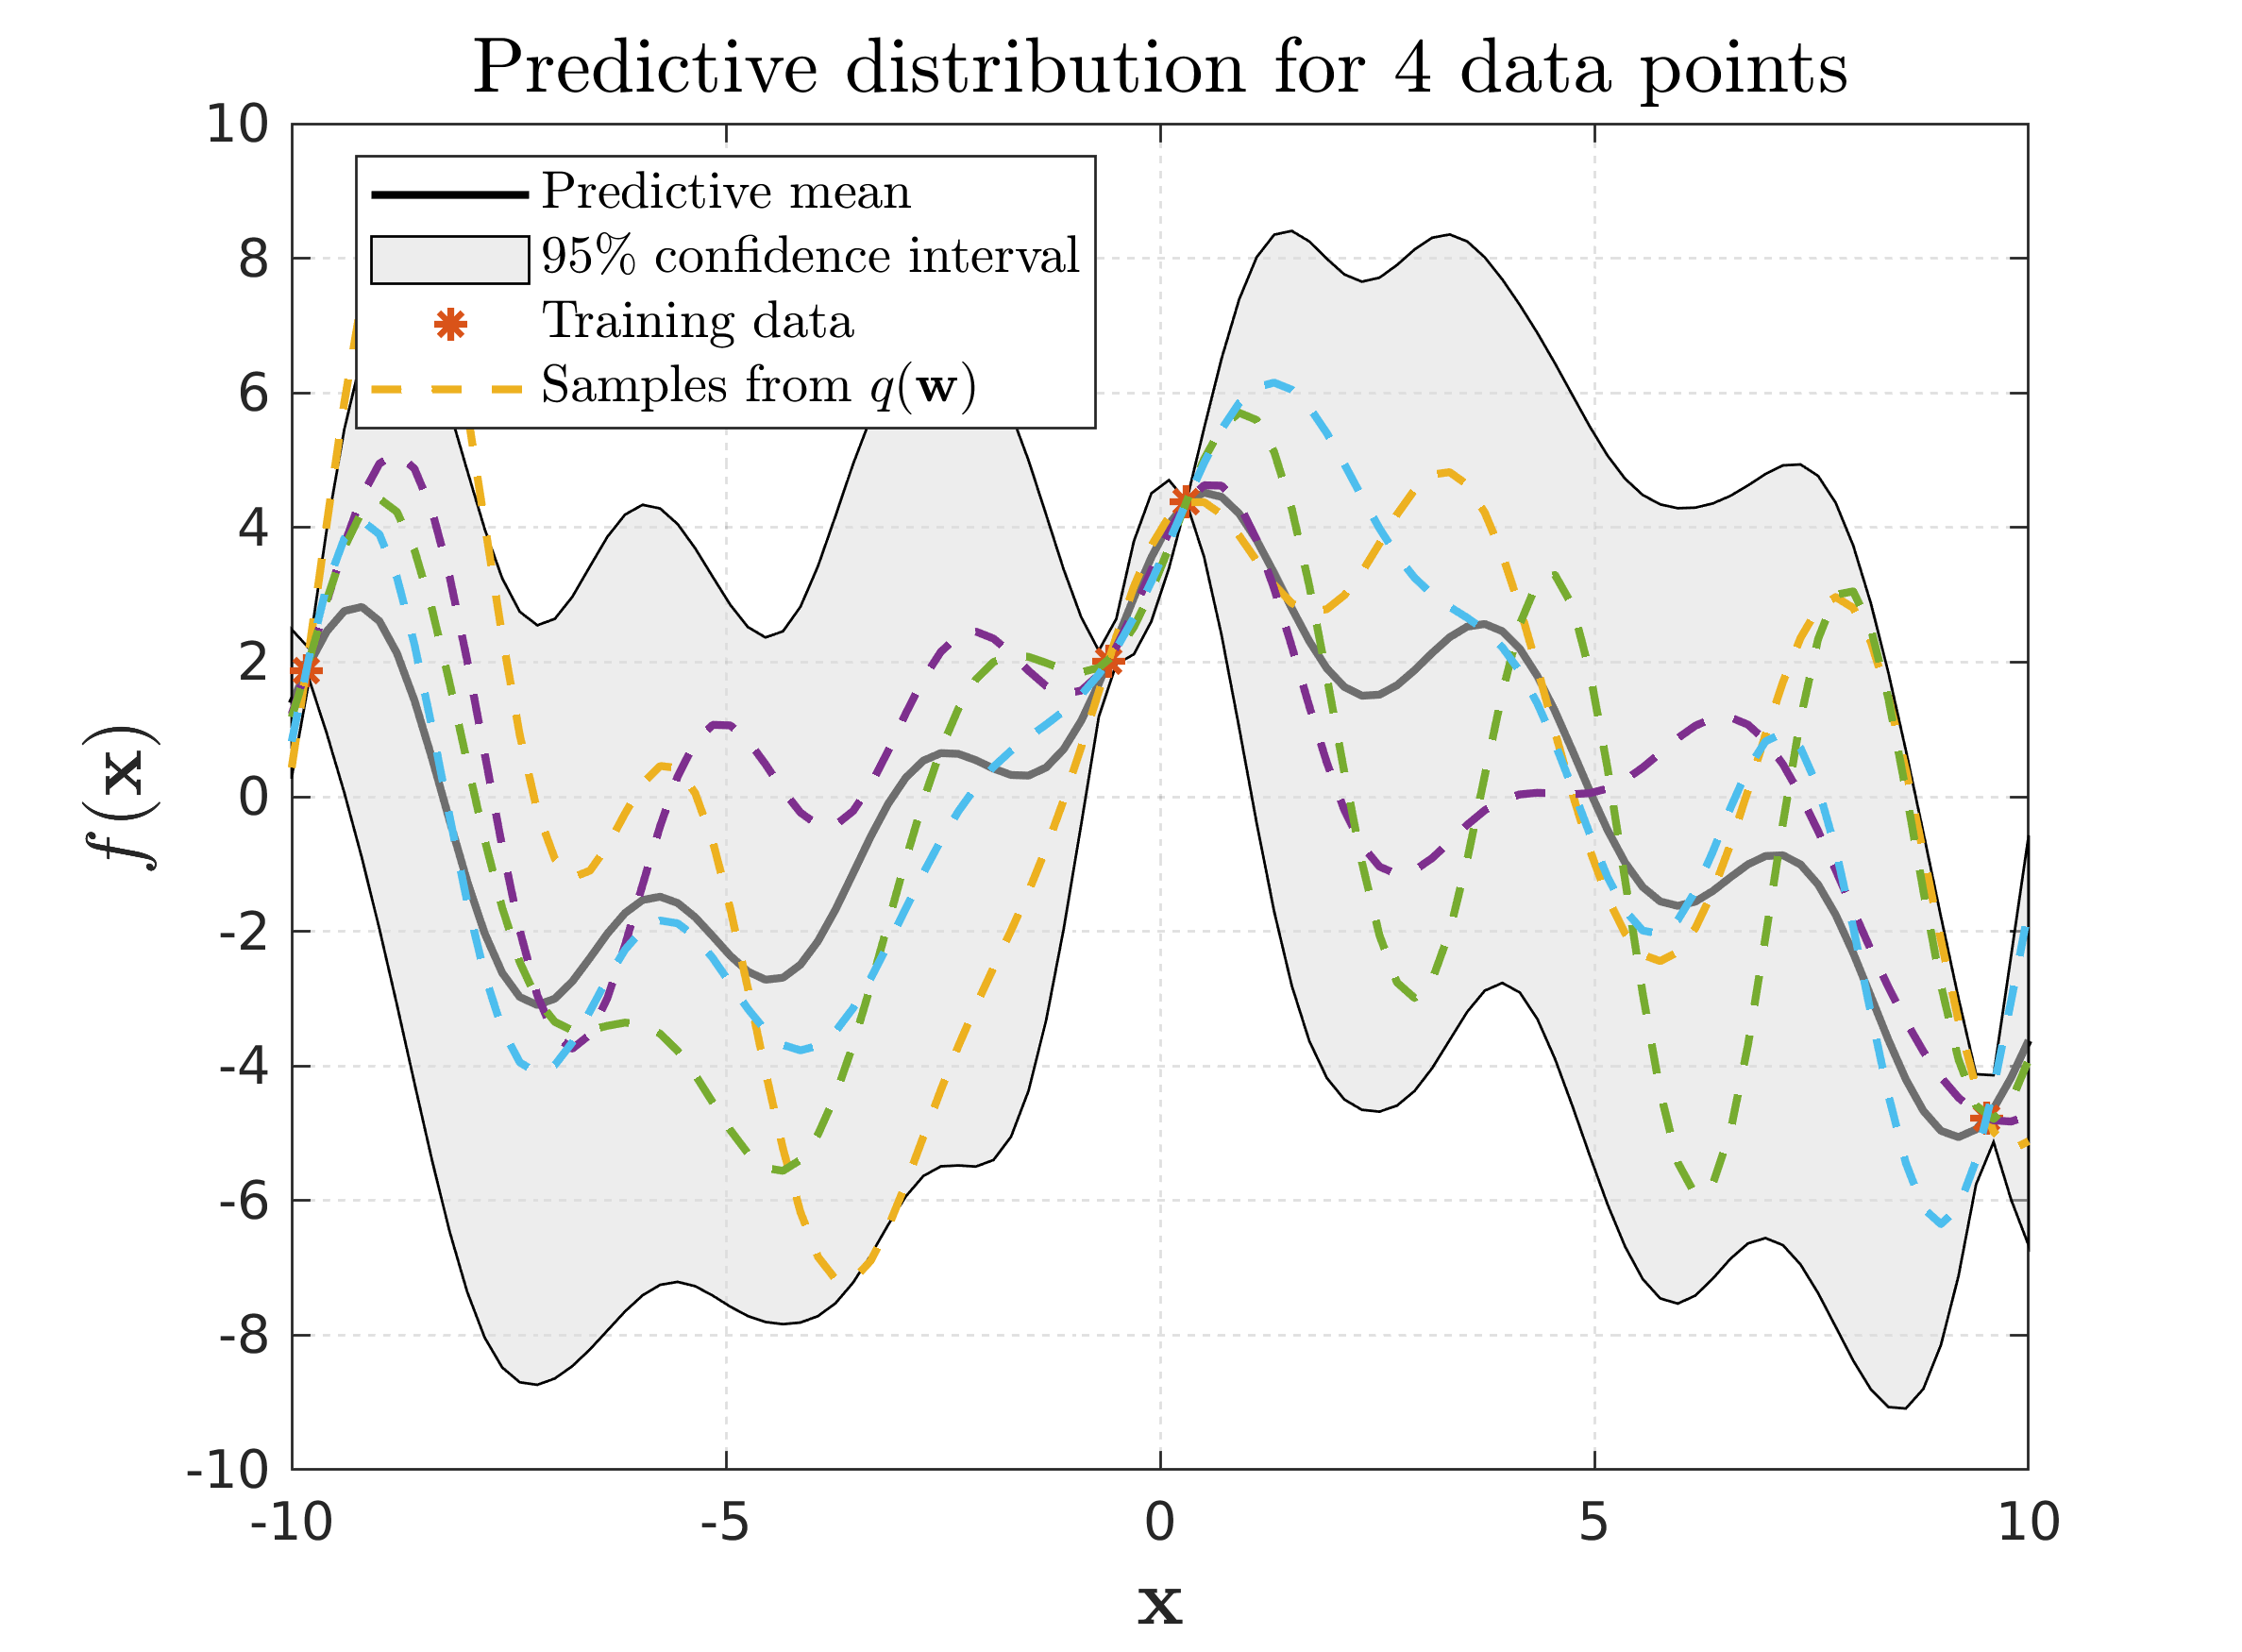
\includegraphics[trim={0 0.18cm 0 0.70cm},clip,height=0.27\textheight,width=0.75\textwidth]{Chapter3/Figures/func_uncertainty_1.png} 
    \caption{Predictive distribution for 4 data points} 
    \label{Fig:Re-pred-4-points} 
  \end{subfigure}

  \begin{subfigure}[b]{0.95\linewidth}
    \centering
    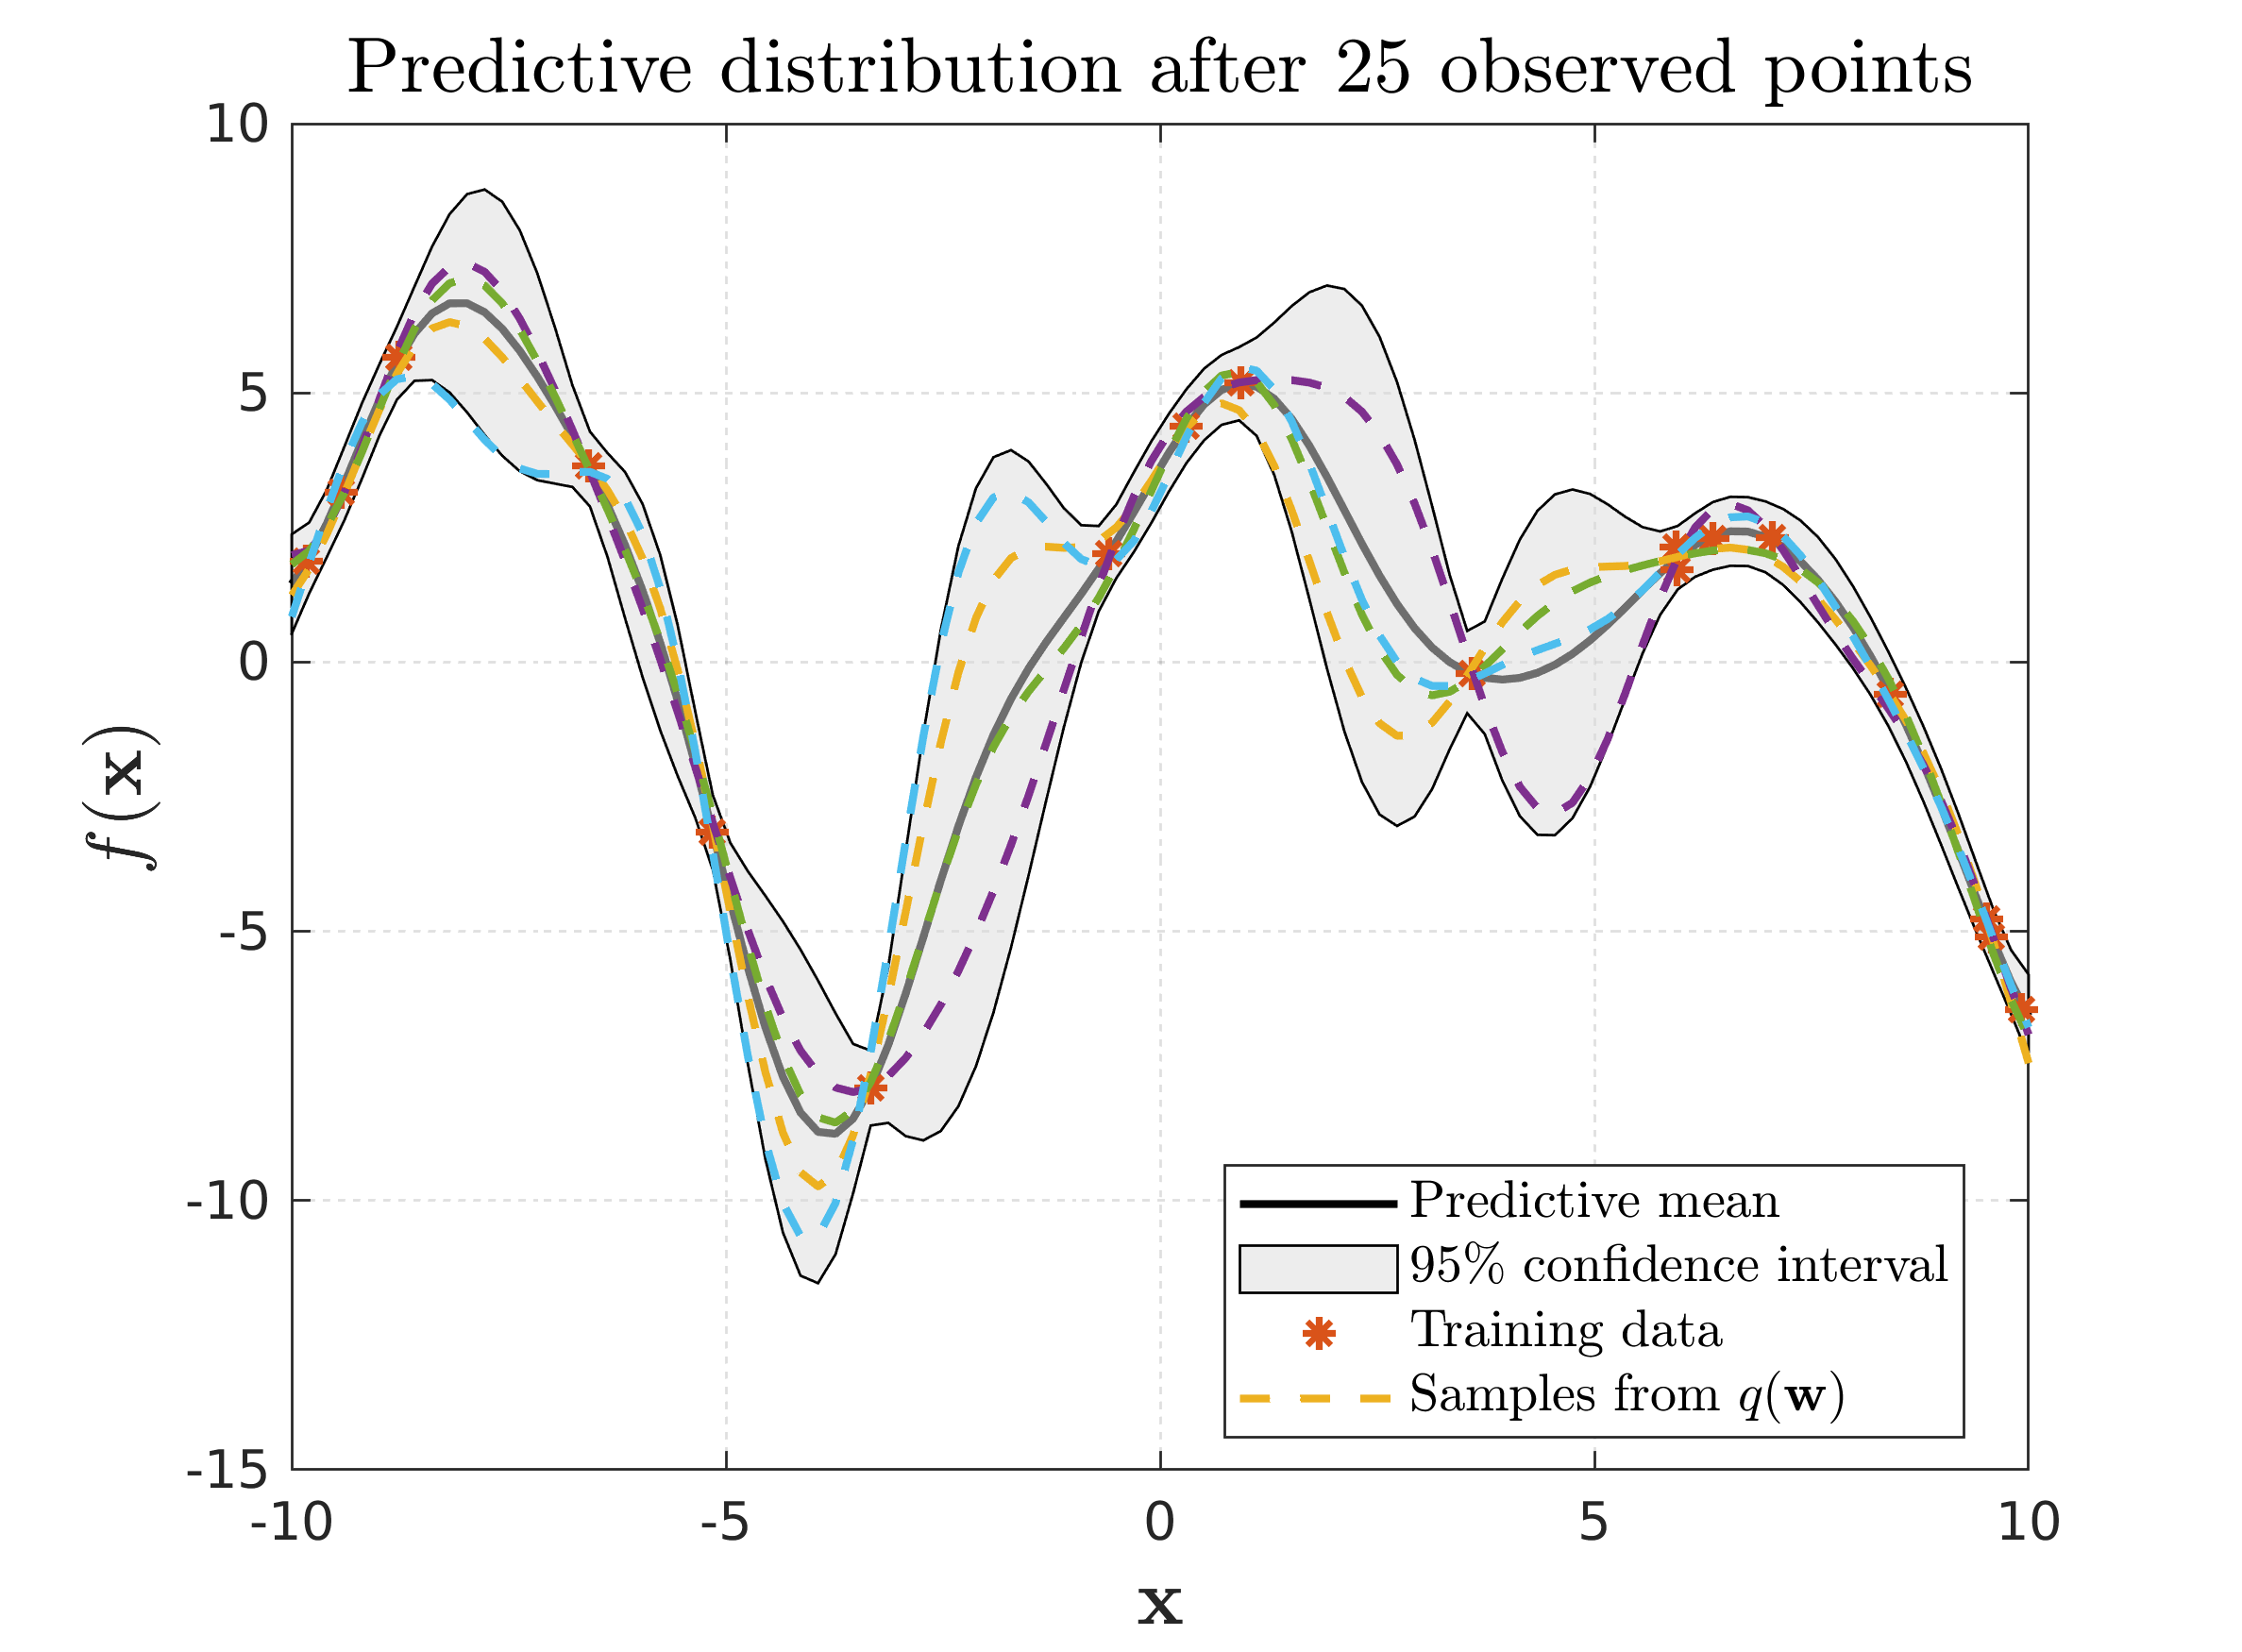
\includegraphics[trim={0 0.18cm 0 0.70cm},clip,height=0.27\textheight,width=0.75\textwidth]{Chapter3/Figures/func_uncertainty_2.png} 
    \caption{Predictive distribution after 25 data points} 
    \label{Fig:Re-pred-25-points}
  \end{subfigure}
  
  \begin{subfigure}[b]{0.95\linewidth}
    \centering
    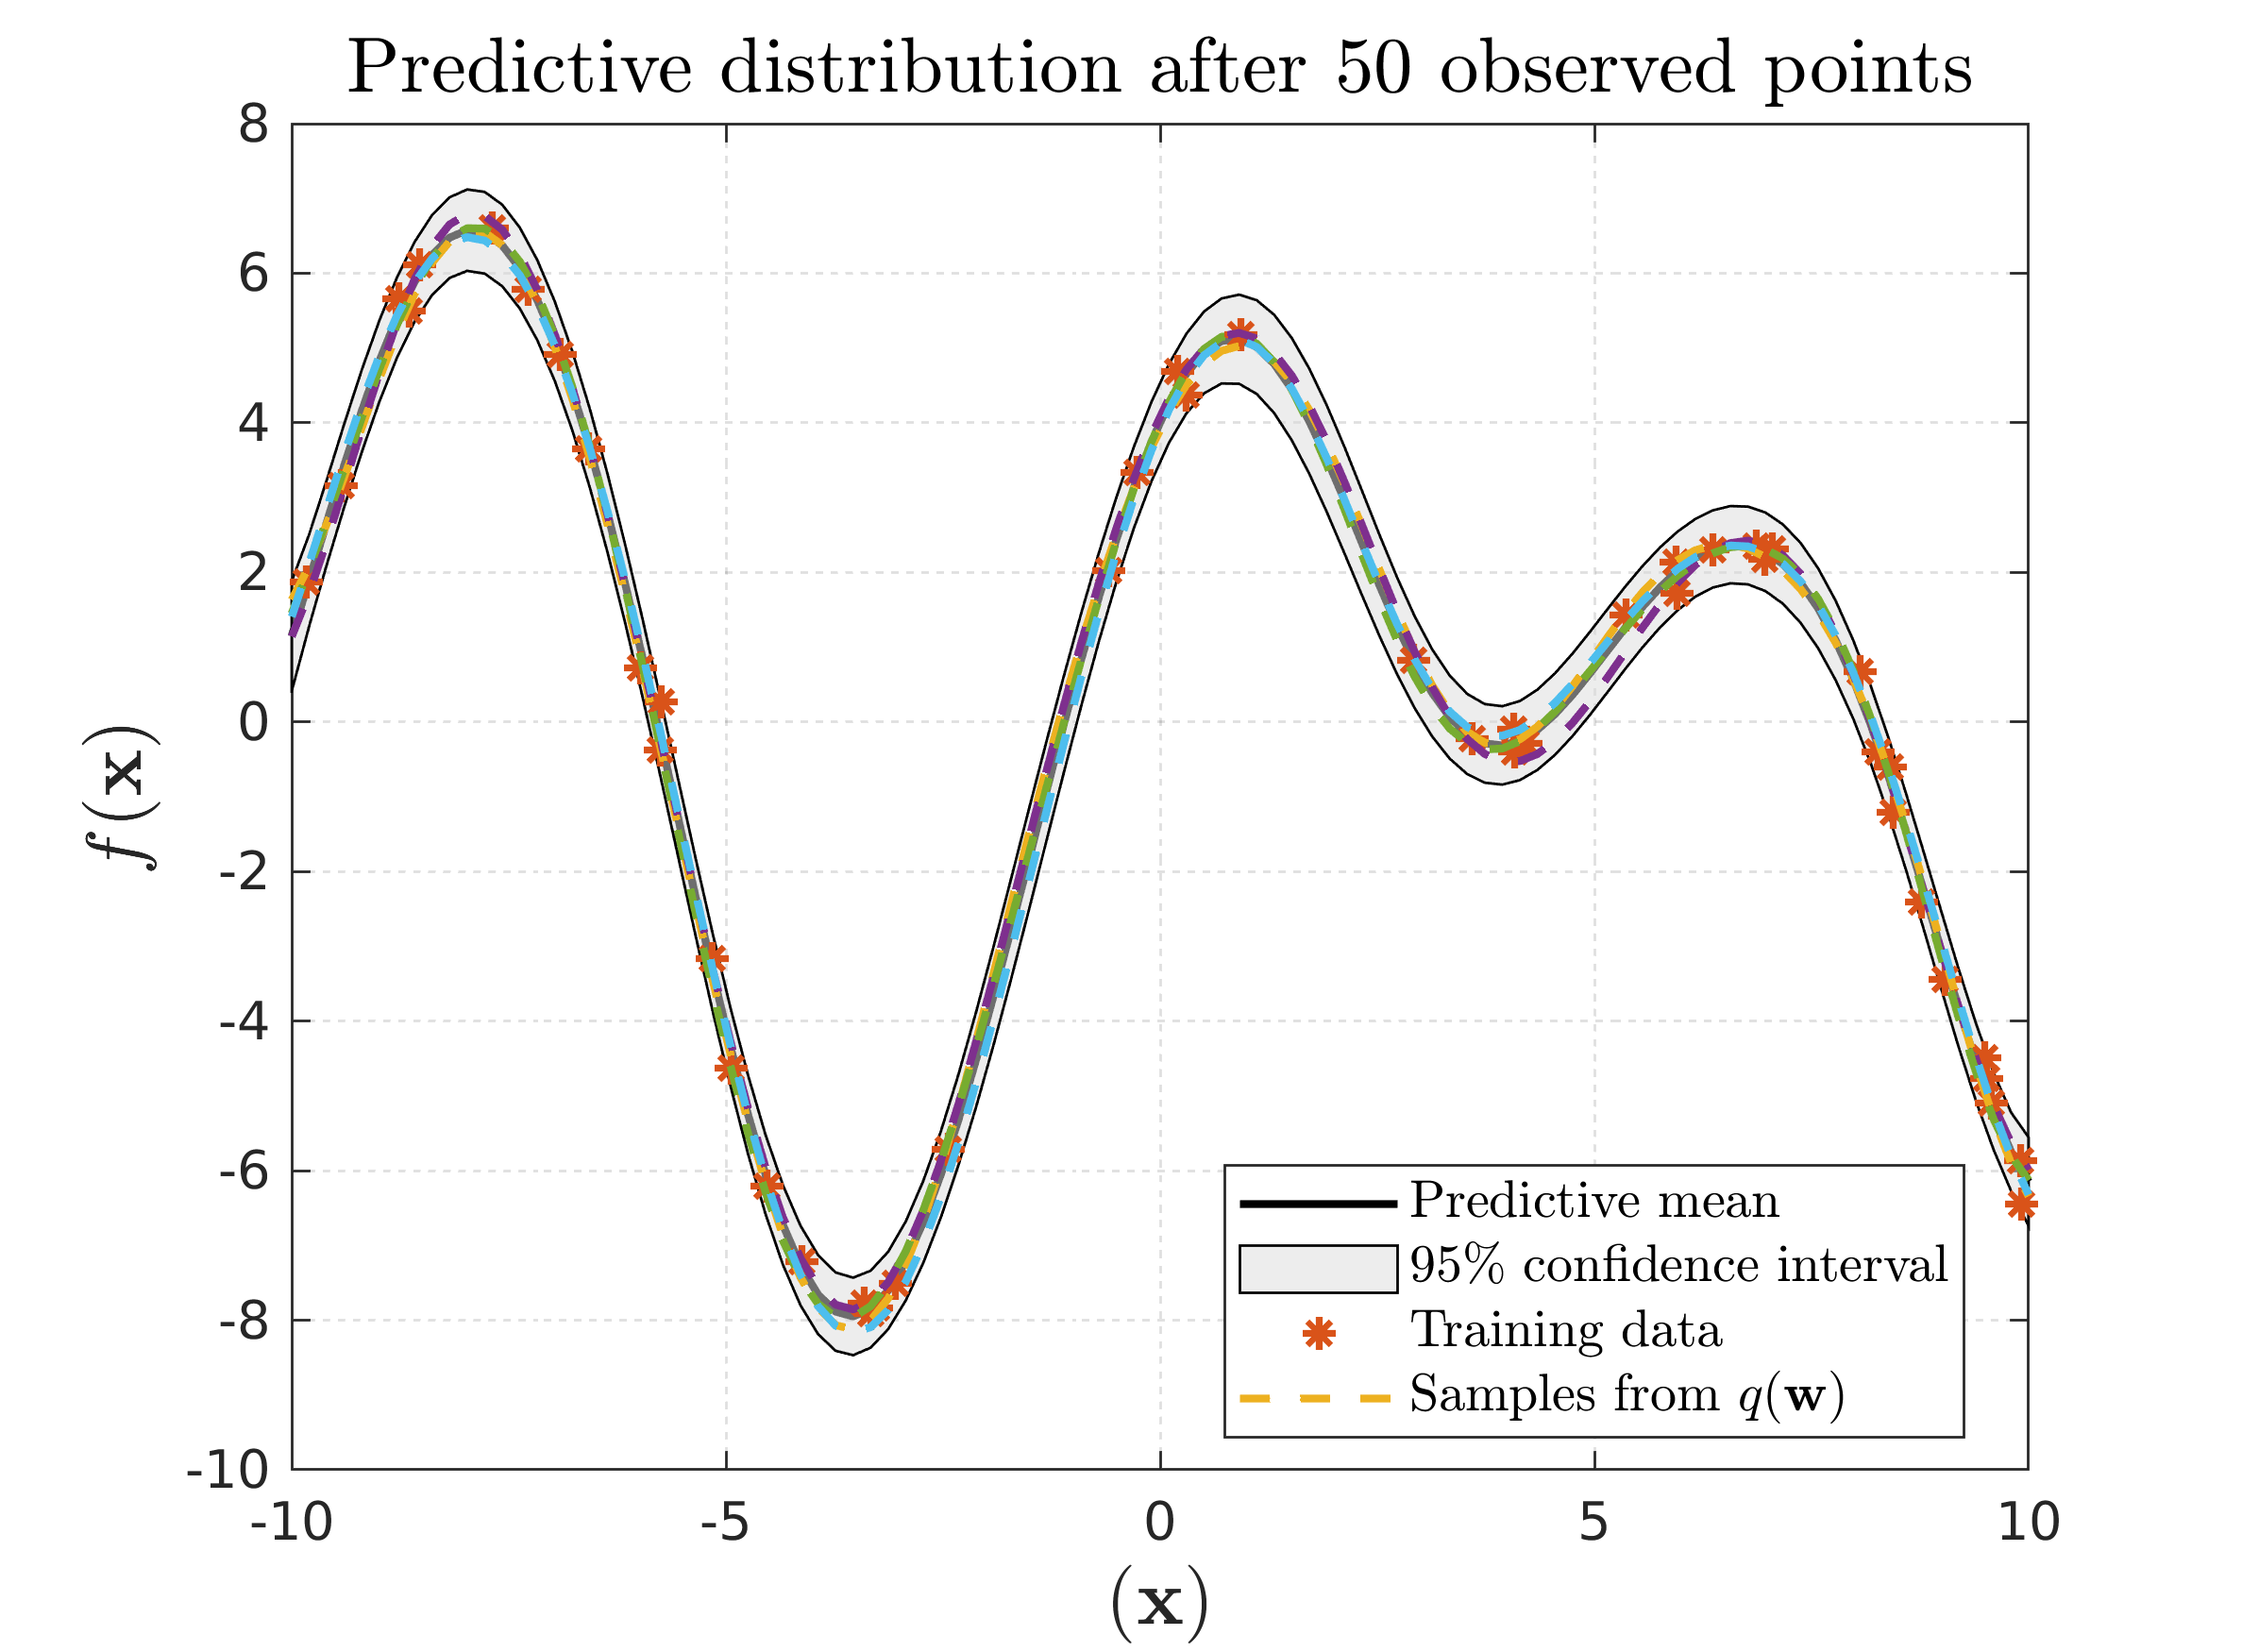
\includegraphics[trim={0 0.1cm 0 0.70cm},clip,height=0.27\textheight,width=0.75\textwidth]{Chapter3/Figures/func_uncertainty_3.png} 
    \caption{Predictive distribution after 50 data points} 
    \label{Fig:Re-pred-50-points}
  \end{subfigure}
 
\caption[Reduction in epistemic uncertainty with added data]{: Fig \ref{Fig:Re-pred-4-points} - \ref{Fig:Re-pred-50-points} show the predictive distribution over the data and samples from the posterior after 4, 25 and 50 observed data points. The lengthscale of the spectral points is purposely set to a high value to over fit the data and imitate high dimensional space. As more data is observed the model becomes increasingly confident about the parameter values and as a consequence the posterior distribution narrows.}
\label{Fig:Re-predictive-fit-to-varying-number-of-datapoints} 
\end{figure}

\begin{figure}[htp!]
\centering    
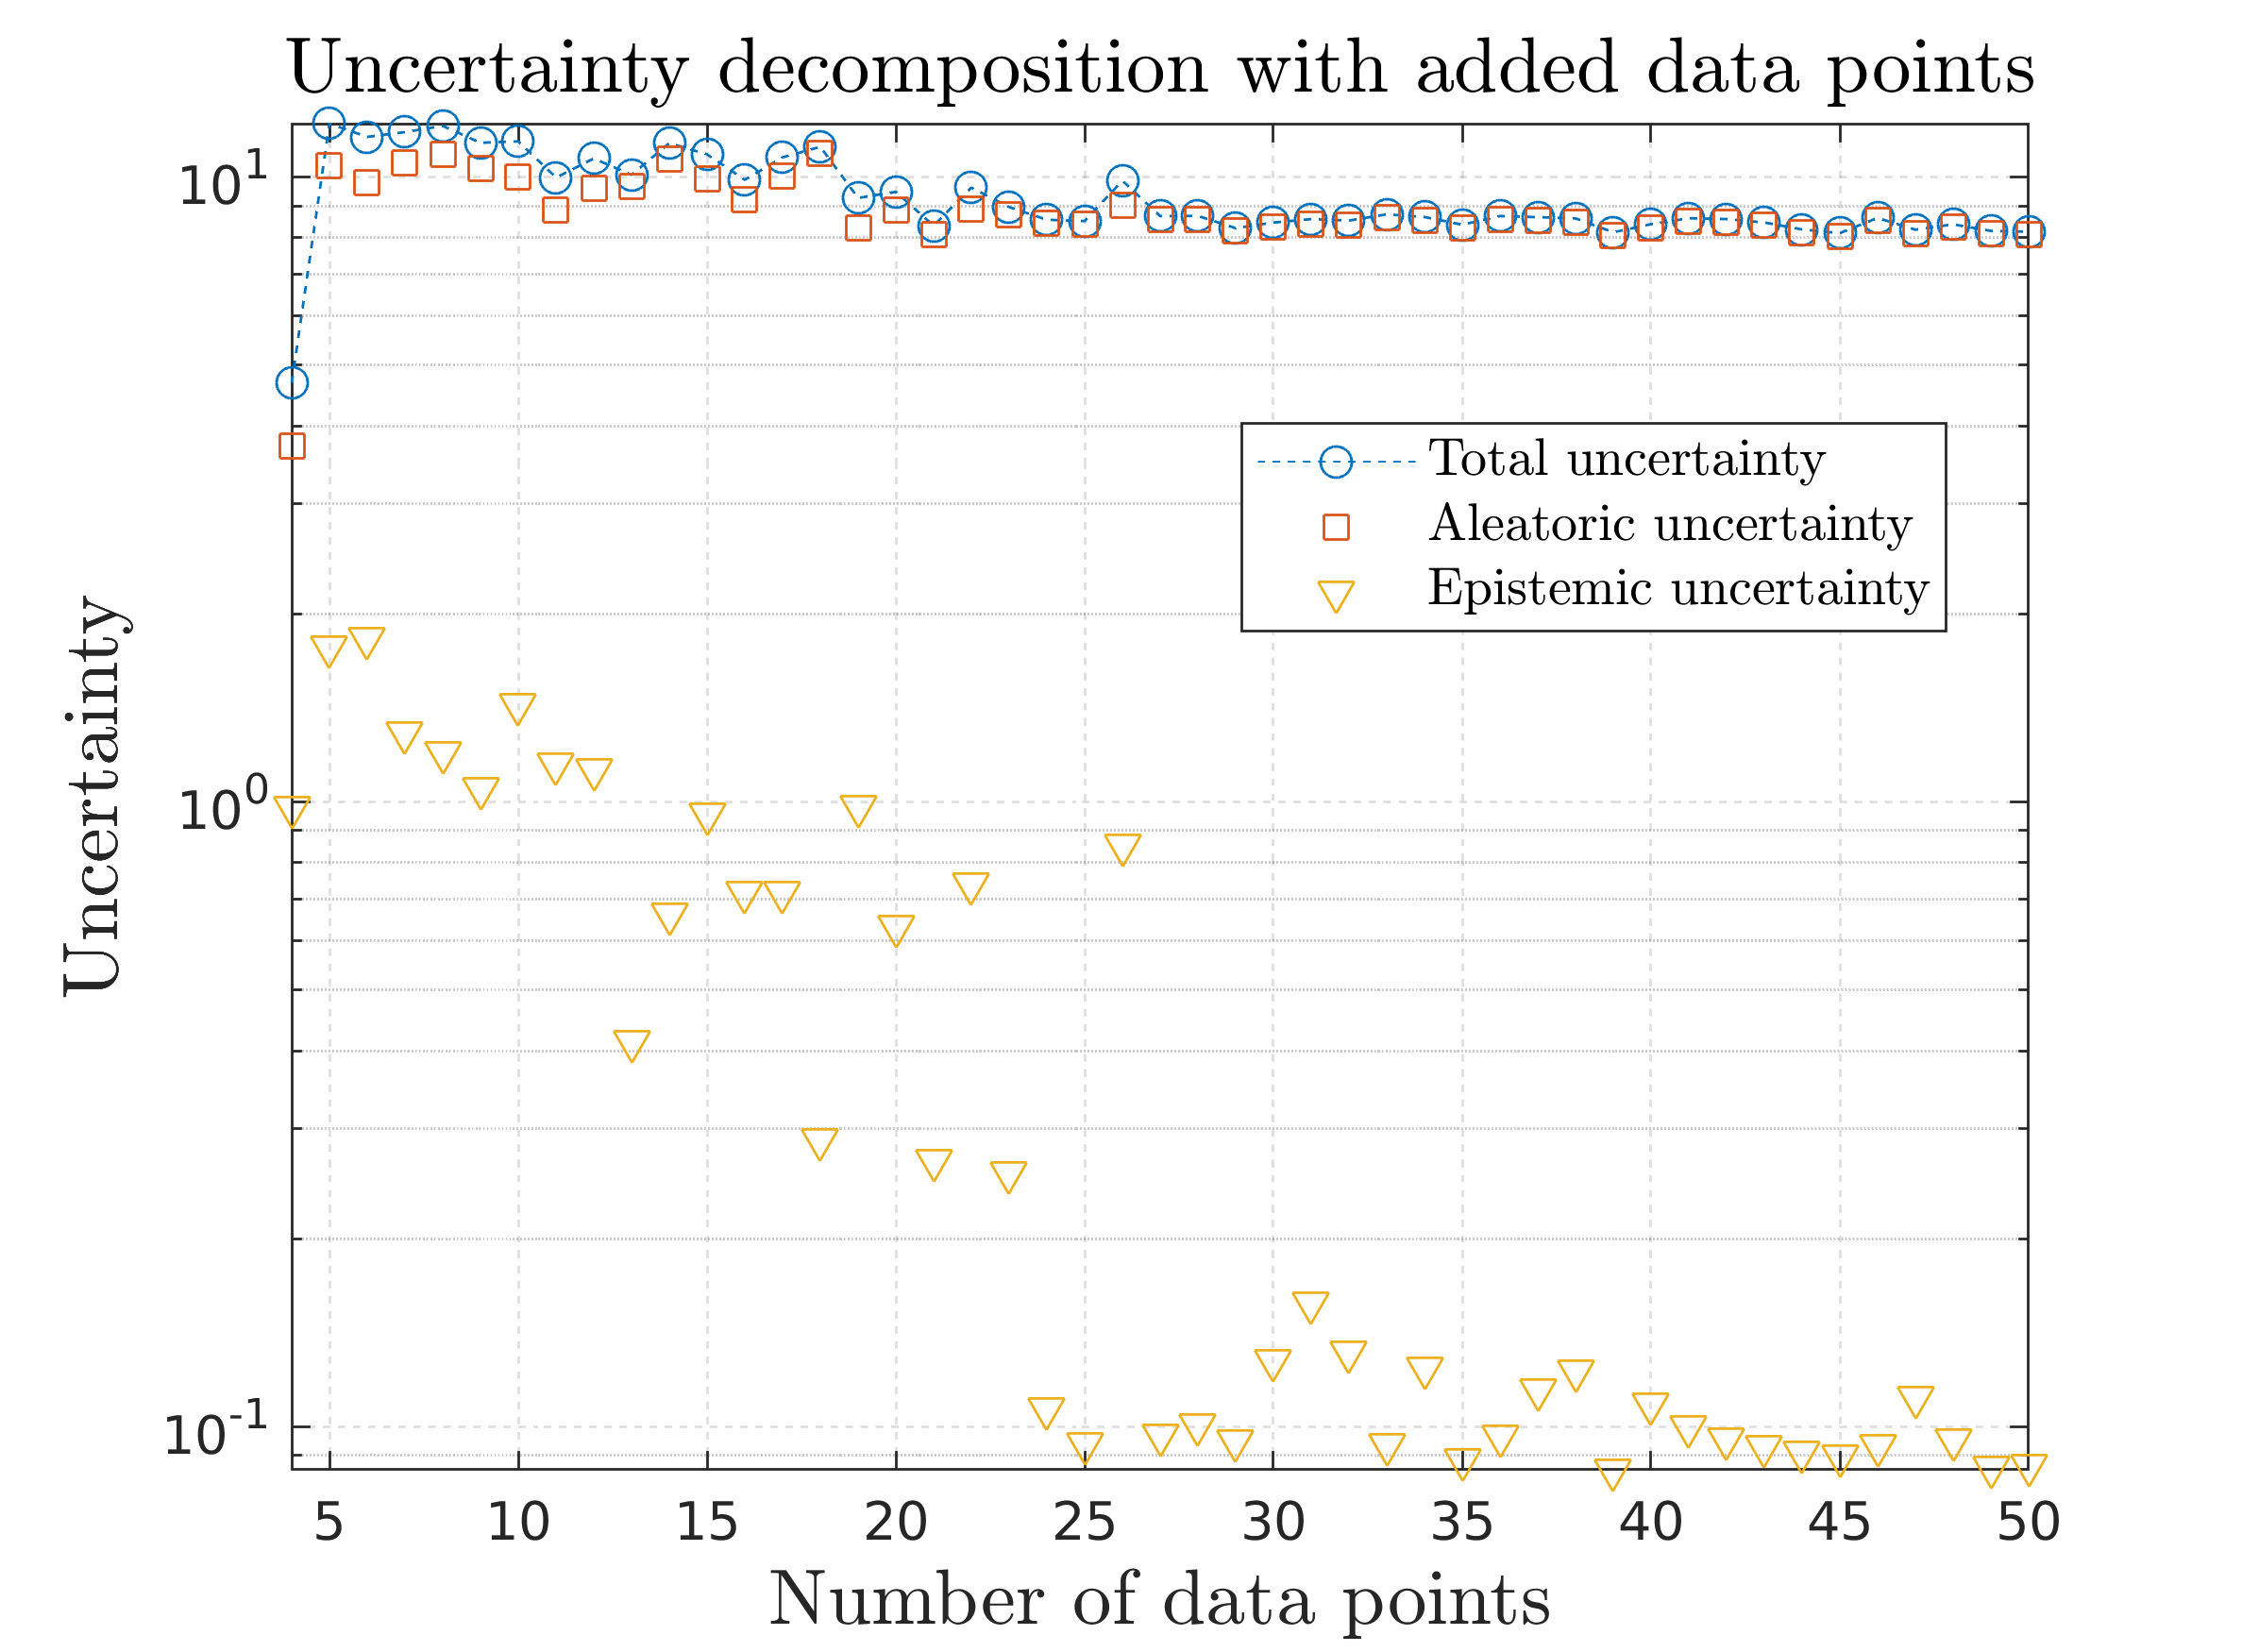
\includegraphics[width=1\textwidth]{Chapter3/Figures/func_uncertainty_4.png}
\caption[Uncertainty decomposition showing reduction in epistemic uncertainty with increasing number of data points]{Relating to Fig. \ref{Fig:Re-predictive-fit-to-varying-number-of-datapoints}. Trajectory roll outs are performed through the transition function each time a new data point is observed (from 4 to 50). For each roll out the uncertainty in the cost is decomposed. As more data is observed the model becomes increasingly confident about its parameters and consequently the epistemic uncertainty reduces due to contraction of the posterior distribution.}
\label{Fig:Re-reduction-in-epsitemic-with-more-data}
\end{figure}


\subsection{The Effect of Cost Uncertainty on Learning}
In this section, Monte-Carlo uncertainty analyses  are presented for the 3 PILCO environments introduced in Sec. \ref{S:PILCO-environments}. The procedure to produce the results is as follows. After each PILCO episode, the trigonometric basis function model is trained on all the observed data up to the end of that episode. The inputs are state-action tuples and the targets are the state differences. Conditionally independent models are trained for each target dimension. In all cases, 500 basis functions are used. Monte-Carlo trajectory roll outs are performed according to Algorithm \ref{GSMCUE:algorithm} under policy $\pi$ for $(M=100,\:N=100,\:T=T_{E})$ where $T_{E}$ and the transition noise $\boldgreek{\varepsilon}_{E}$ are environment specific. The uncertainty is then decomposed into uncertainties which represent the total aleatoric and total epistemic uncertainty in the cost $\mathbb{C}(\mathbf{x})$ under policy $\pi$ for an entire episode.   

For each environment, figures are produced that show:
\begin{itemize}
    \item a random sample of the Monte-Carlo trajectory roll outs for each of the state variables that describe the environment. For each figure the left axis represents the state variable and corresponds to trends for the Monte-Carlo trajectories, the actual trajectory recorded during that episode, the target of the state variable and PILCO's prediction of the state evolution before the episode. The right axis shows the percentage of Monte-Carlo trajectories that fall within the 2 standard deviation error bars of PILCO's prediction for that time step;
    \item the average cost and cost uncertainty decomposition under policy $\pi$ for each each episode. The average cost per episode is shown of the left axis which is indicative of learning. High cost indicates that the agent is not achieving the objective, low cost indicates the objective is being achieved and a decreasing average cost indicates the agent is learning. The right axis shows total cost uncertainty and its decomposition into aleatoric epistemic cost uncertainty;
    \item the average cost and the ratio of epistemic cost uncertainty to total cost uncertainty under policy $\pi$ for each each episode. The left axis shows the average cost and the right axis the ratio of epistemic cost uncertainty to total cost uncertainty.
\end{itemize}

\subsubsection{Cart-pole}
Fig. \ref{Fig:Re-cp-MC-roll-outs-1} and \ref{Fig:Re-cp-MC-roll-outs-2} show a random sample of the Monte-Carlo trajectory roll outs for the state variables of the cart-pole environment: cart position $x$, cart velocity $\dot{x}$, pendulum angular velocity $\dot \theta$ and pendulum angle $\theta$. The trajectories shown in the figures are from episode 15, when PILCO has achieved the environment objective, and so represent trajectories under a mature policy $\pi$.  For the cart-pole environment, a high agreement, approximately greater than $80\%$, is noted between the Monte-Carlo trajectories and PILCO's prediction of the state evolution.

Fig. \ref{Fig:Re-cp-full-uncertainty} shows the average cost per episode and the uncertainty in the cost over the course of learning. The average cost per episode exhibits a sharp decline early in the learning process (shown in both figures) and by the third episode PILCO has solved the environment. This is the simplest of the environments tested and because PILCO solves it early in the learning process, not much insight into how the cost uncertainty varies is gained. In episode zero (not shown in the figures), PILCO performs a series of roll outs under a random policy to generate initial state observations. It is likely, particularly in the case where the state-space is well explored during the random roll out, that these data are enough for the algorithm to find a low cost policy that solves the environment early in the learning process. Consequently, for episodes 1-3 the selected policy contains little epistemic cost uncertainty because the model is already confident about its beliefs and a successful low cost policy exists. Interestingly, for episodes 7 and 8, PILCO selects policies with high epistemic uncertainty in the cost and does so after it has already solved the environment. This could be due to PILCO's unintentional exploration mechanism where it favours uncertain states. After this (Fig. \ref{Fig:Re-cp-uncertainty} episodes 9-15), the total and aleatoric uncertainties settle and the epistemic reduces, indicating that the model is now confident in its model of parts of the state-space associated with low cost.

% \begin{table}
% \caption{Even better looking table using booktabs}
% \centering
% \label{table:good_table}
% \begin{tabular}{l c c c c c c}
% \toprule
% \multirow{2}{*}{State variable} & \multicolumn{2}{c}{Cart-pole} & \multicolumn{2}{c}{Pendubot}  &
% \multicolumn{2}{c}{Cart-double-pendulum}  \\ 
% \cmidrule{2-7}
%   & Start & Target & Start & Target & Start & Target \\ 
% \midrule
% Cart position $x_1$ & & & & & & \\

% Cart velocity $\dot x_1$ & & & & & & \\

% Angle 2 $\theta_2$ & & & & & & \\

% Angle 3 $\theta_3$ & & & & & &\\

% Angular velocity 2 $\dot \theta_2$ & 13.47 & 0.09 & 10.55 & 0.05 & &\\

% Angular velocity 3 $\dot \theta_3$ & 11.88 & 0.05 & 13.11 & 0.04& &\\ 
% \bottomrule
% \end{tabular}
% \end{table}

\begin{figure}[H]    
   \begin{subfigure}[b]{1\linewidth}
    \centering
    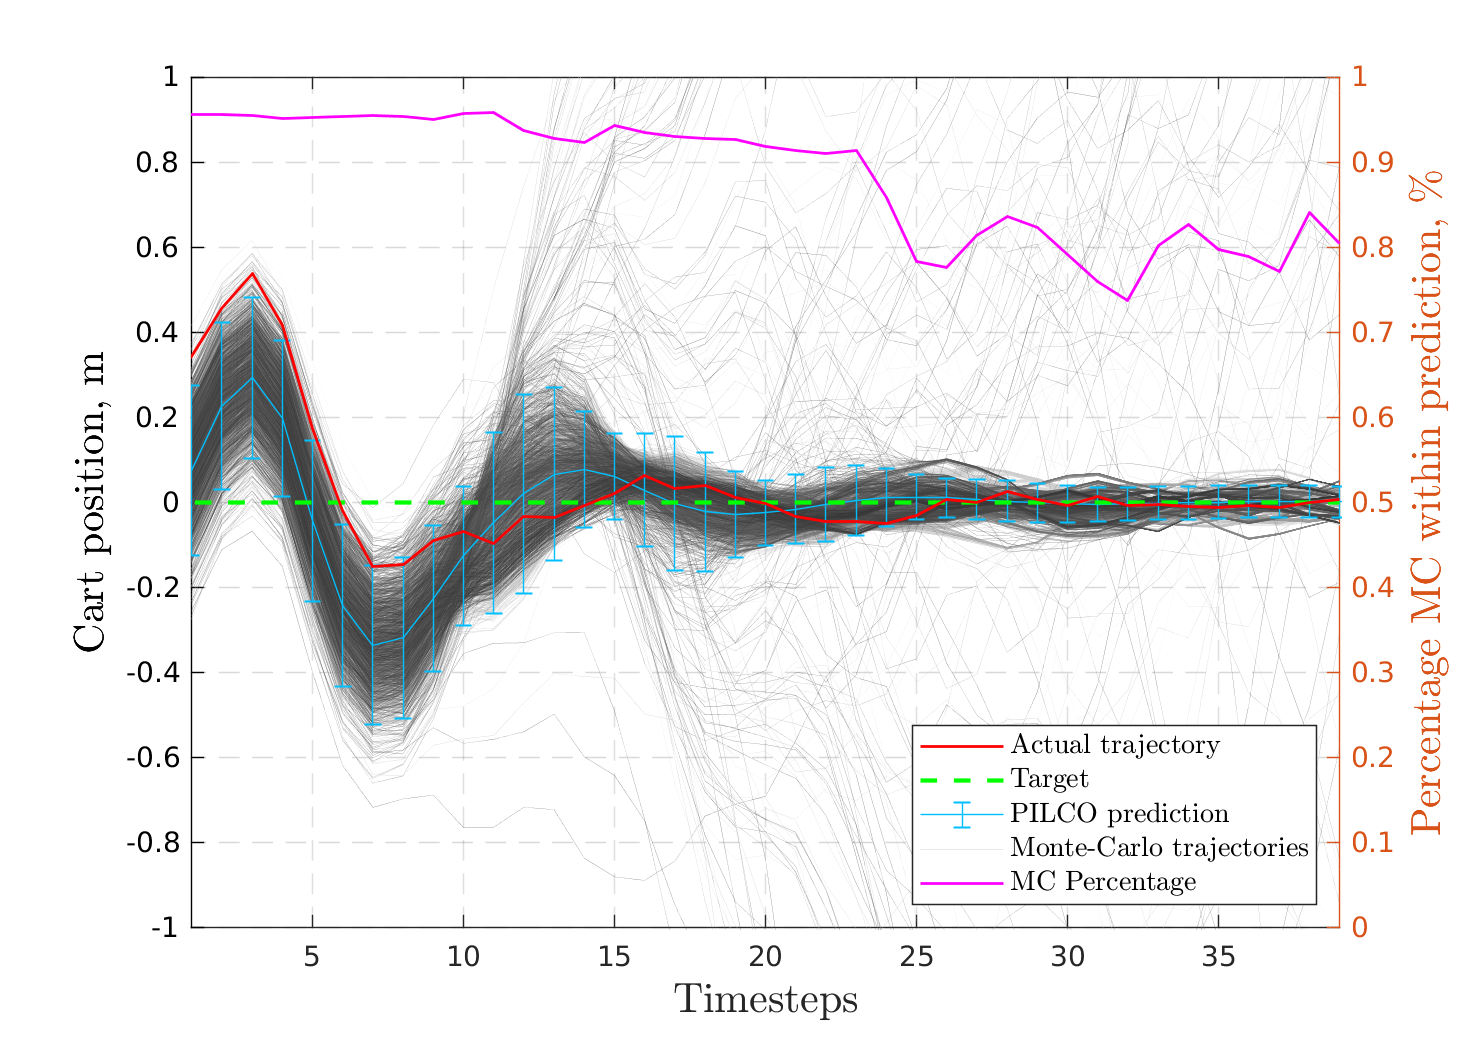
\includegraphics[height=0.4\textheight,width=1\textwidth]{Chapter3/Figures/cp_MC_rollout_Ep_15_Dim_1.png} 
    \caption{Cart position $x$ (m)} 
    \label{Fig:Re-cp-cart-position} 
  \end{subfigure} 
  \begin{subfigure}[b]{1\linewidth}
    \centering
    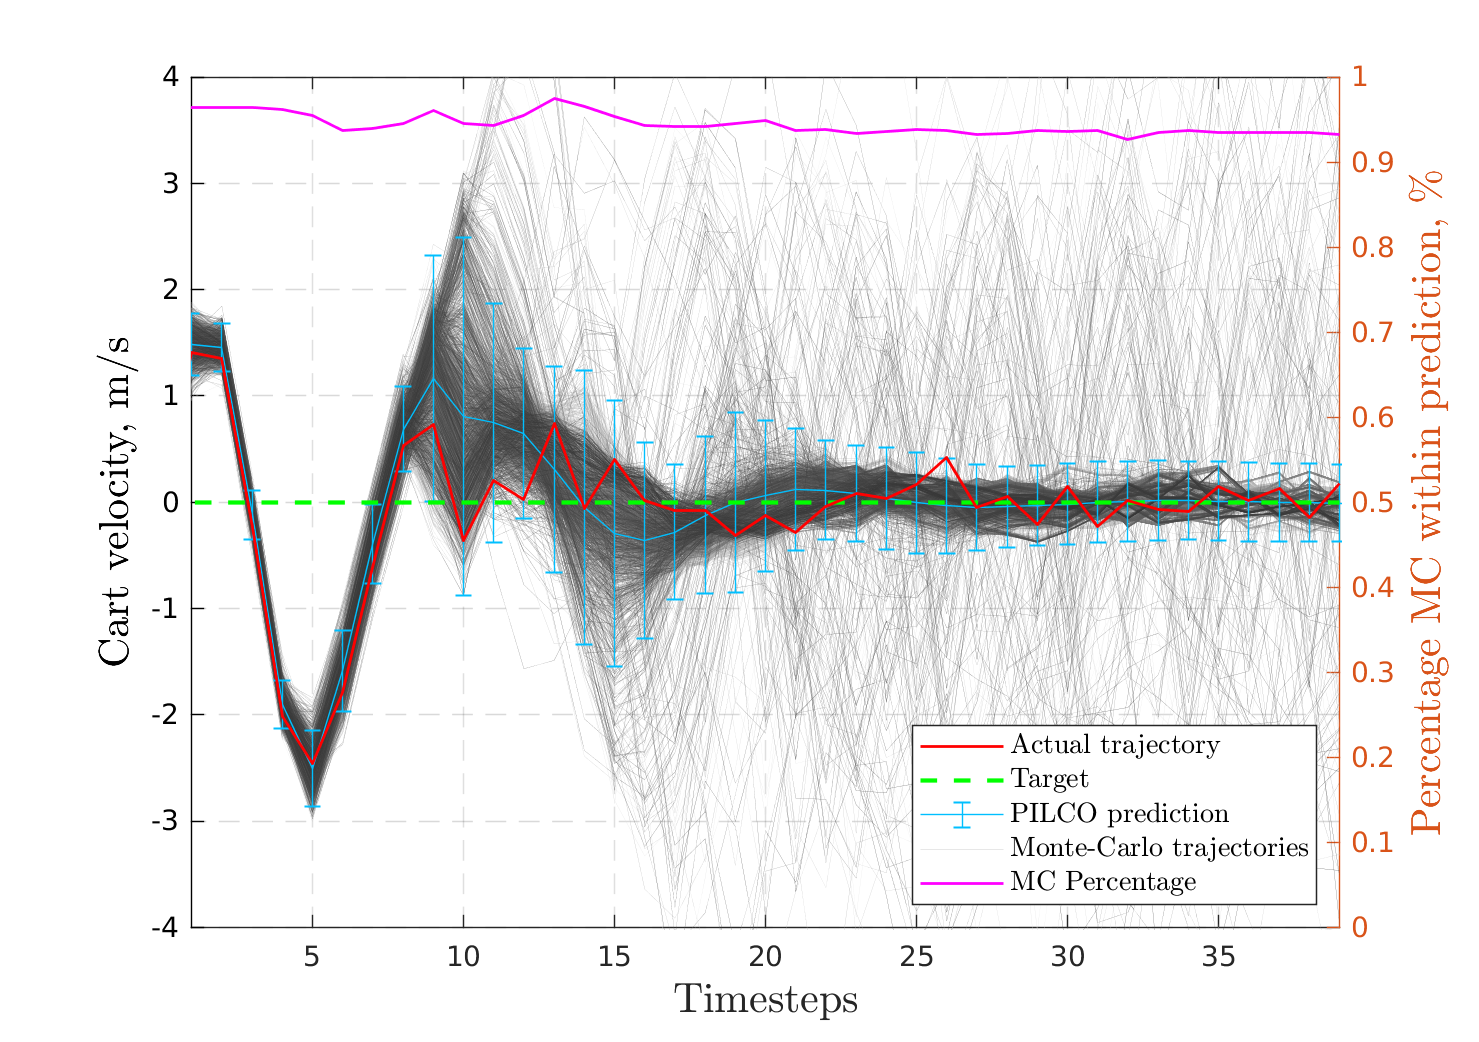
\includegraphics[height=0.4\textheight,width=1\textwidth]{Chapter3/Figures/cp_MC_rollout_Ep_15_Dim_2.png} 
    \caption{Cart velocity $\dot x$ (m/s)} 
    \label{Fig:Re-cp-cart-velocity} 
  \end{subfigure} 
\caption[Monte-Carlo roll outs for \textbf{cart-pole} cart position and cart velocity]{Monte-Carlo roll outs for the \textbf{cart-pole} environment for cart position and cart velocity. Figures show a random sample of the Monte-Carlo trajectories for episode 15. The first three legend items (actual trajectory, target, PILCO prediction and MC trajectories) correspond to the state variable axis (left axis) and the magenta line shows the percentage of MC trajectories inside PILCO's prediction (2 standard deviations) (right axis). Sample time 0.1s, roll out horizon 4.0s}
\label{Fig:Re-cp-MC-roll-outs-1} 
\end{figure}
 
 
\begin{figure}[H]    
  \begin{subfigure}[b]{1\linewidth}
    \centering
    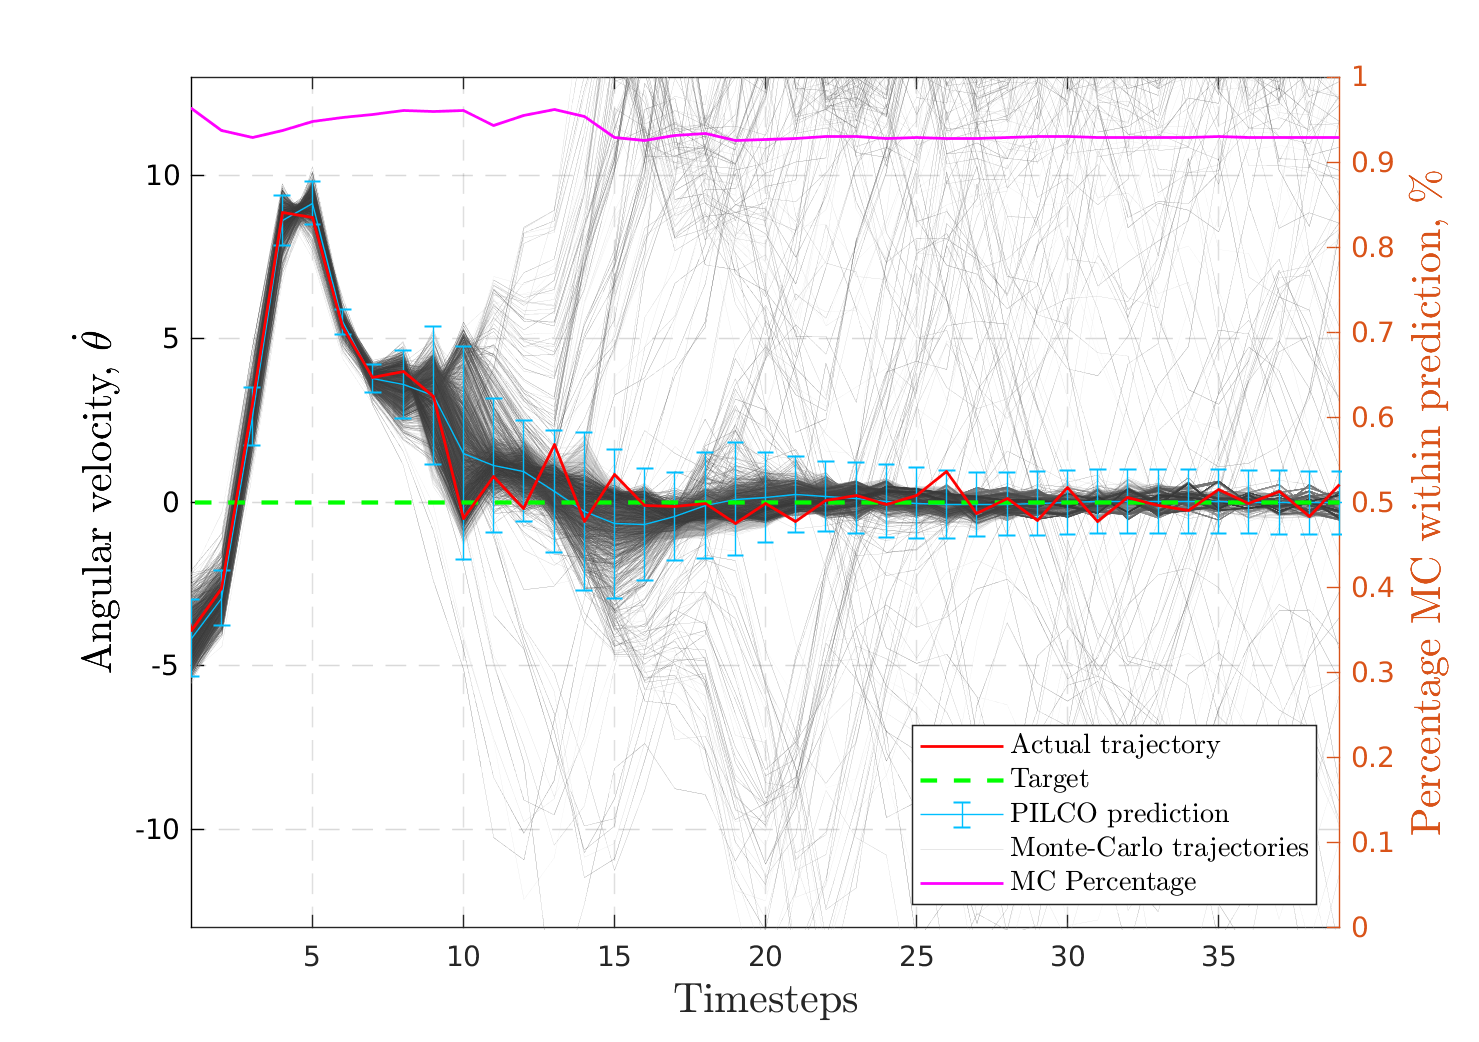
\includegraphics[height=0.4\textheight,width=1\textwidth]{Chapter3/Figures/cp_MC_rollout_Ep_15_Dim_3.png} 
    \caption{Pendulum angular velocity $\dot \theta$ (rad/s)} 
    \label{Fig:Re-cp-pen-velocity} 
  \end{subfigure} 

  \begin{subfigure}[b]{1\linewidth}
    \centering
    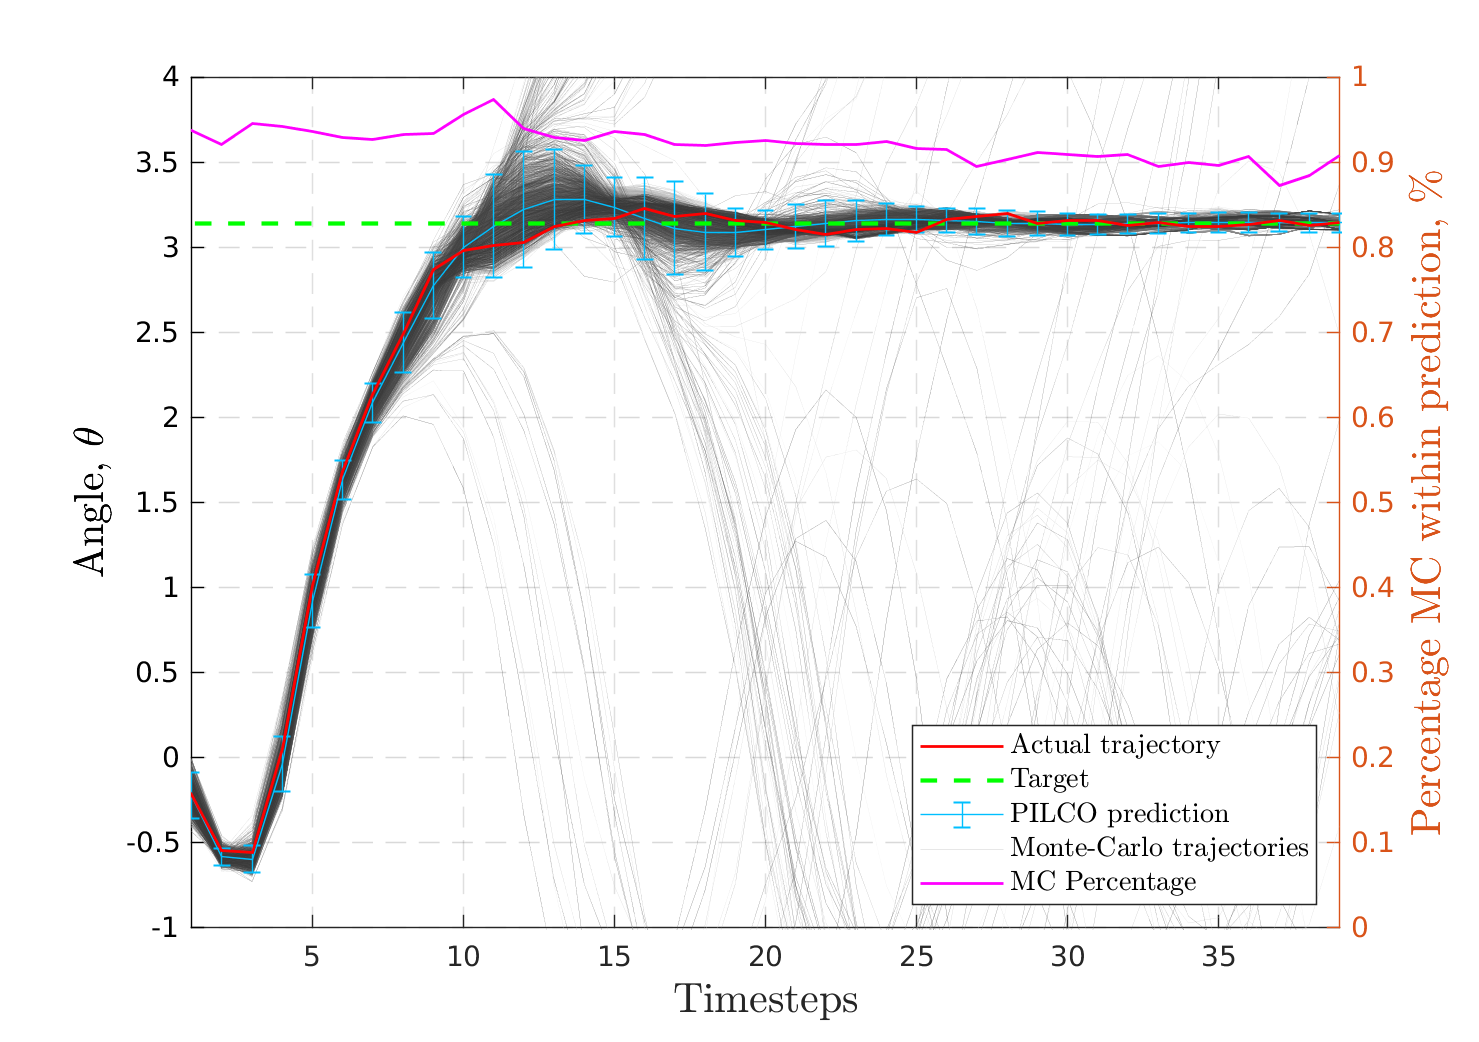
\includegraphics[height=0.4\textheight,width=1\textwidth]{Chapter3/Figures/cp_MC_rollout_Ep_15_Dim_4.png} 
    \caption{Pendulum angle $\theta$ (rad)} 
    \label{Fig:Re-cp-pen-angle} 
  \end{subfigure} 
\caption[Monte-Carlo roll outs for \textbf{cart-pole} pendulum angular velocity and pendulum angle]{Monte-Carlo roll outs for the \textbf{cart-pole} environment for pendulum angular velocity and pendulum angle. Figures show a random sample of the Monte-Carlo trajectories for episode 15. The first three legend items (actual trajectory, target, PILCO prediction and MC trajectories) correspond to the state variable axis (left axis) and the magenta line shows the percentage of MC trajectories inside PILCO's prediction (2 standard deviations) (right axis). Sample time 0.1s, roll out horizon 4.0s}
\label{Fig:Re-cp-MC-roll-outs-2} 
\end{figure}
 
\begin{figure}[H]    
  \begin{subfigure}[b]{1\linewidth}
    \centering
    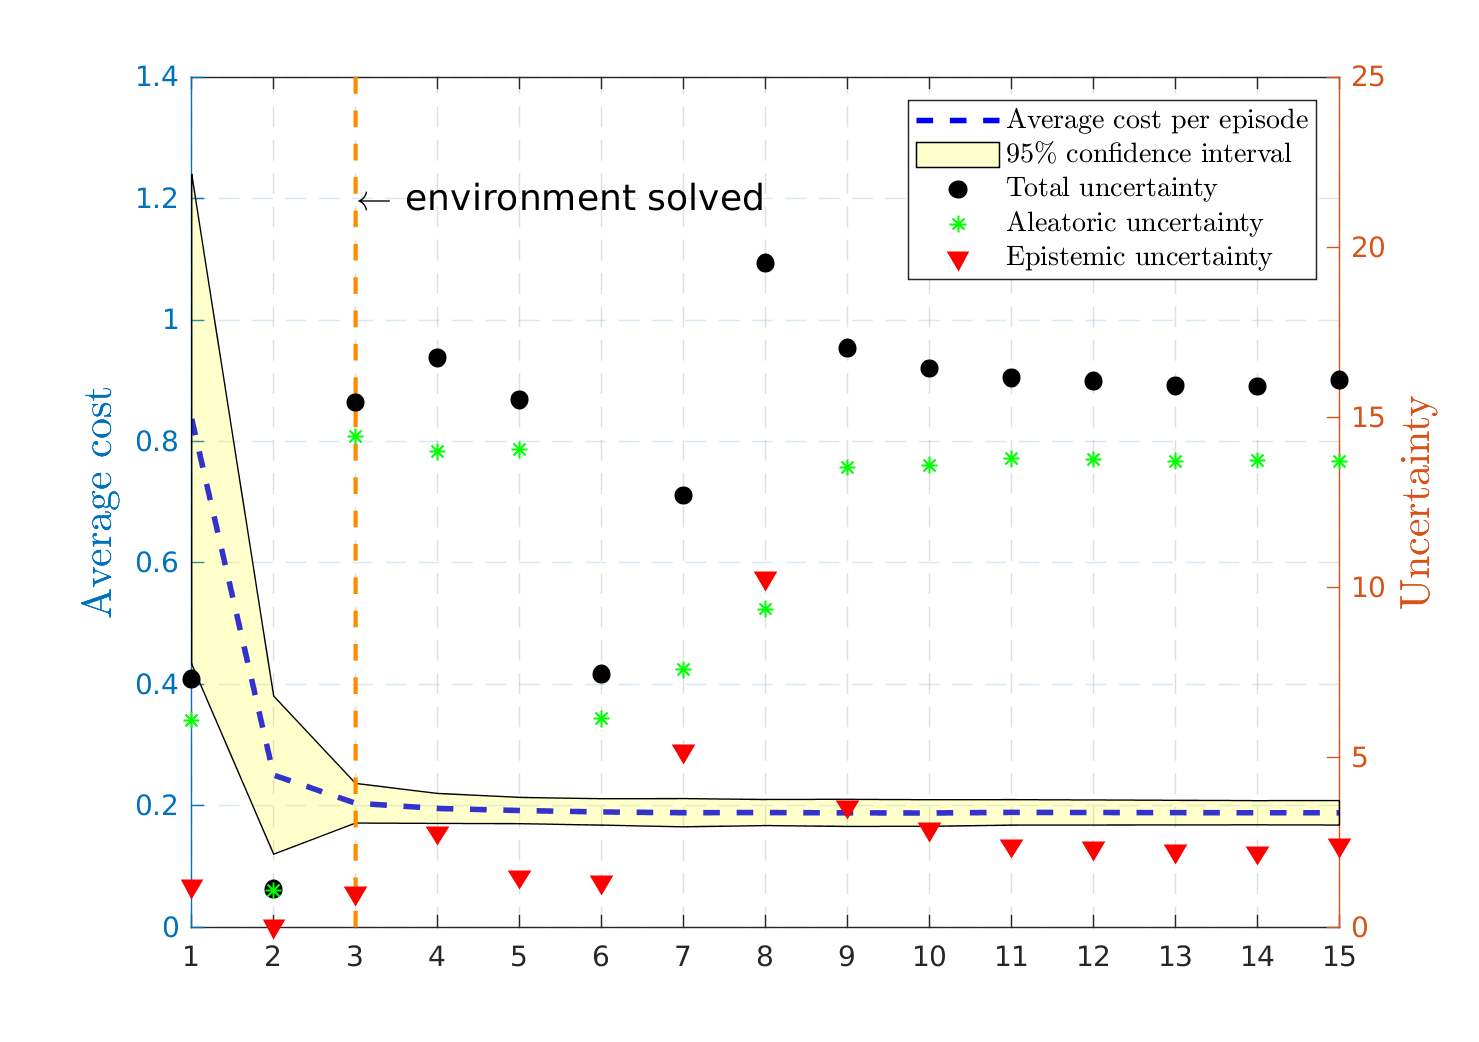
\includegraphics[height=0.4\textheight,width=1\textwidth]{Chapter3/Figures/cp_uncertainty.png} 
    \caption{Average cost (left axis) and uncertainty decomposition (right axis) for each episode over the course of learning.} 
    \label{Fig:Re-cp-uncertainty} 
  \end{subfigure}
  
  \begin{subfigure}[b]{1\linewidth}
    \centering
    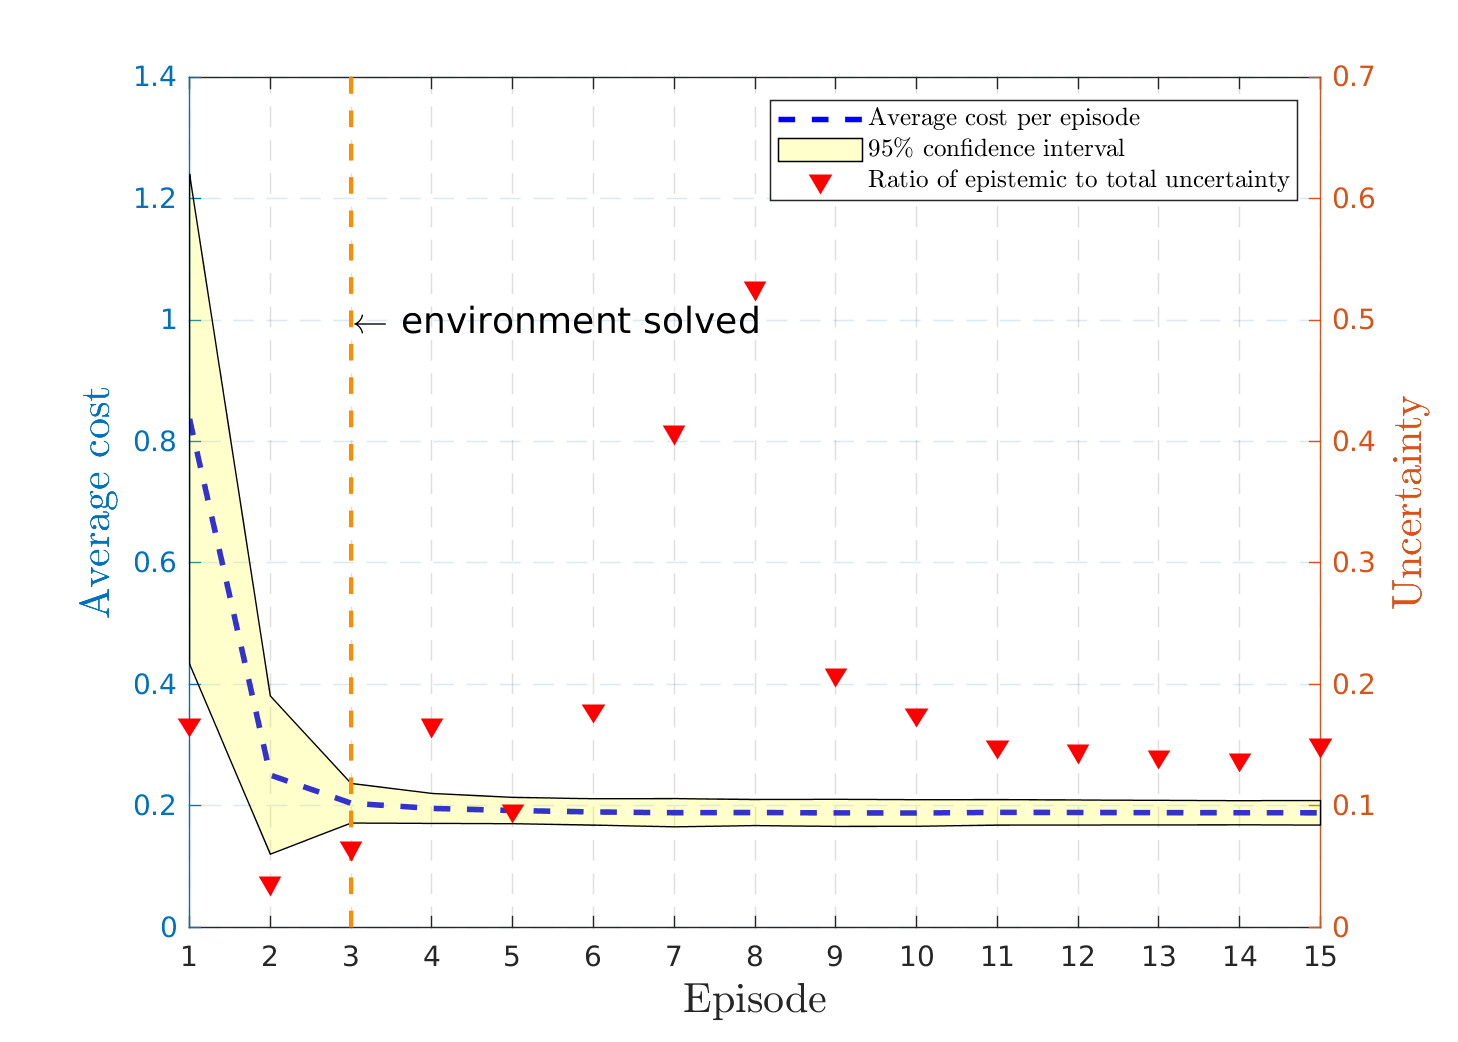
\includegraphics[height=0.4\textheight,width=1\textwidth]{Chapter3/Figures/cp_uncertainty_norm.png} 
    \caption{Average cost (left axis) and ratio of epistemic to total uncertainty (right axis) for each episode over the course of learning.} 
    \label{Fig:Re-cp-uncertainty-norm} 
  \end{subfigure}  
\caption[Uncertainty decomposition for \textbf{cart-pole} environment]{\textbf{Cart-pole}: Average cost (left axis) and uncertainty (right axis) for each episode over the course of learning.}
\label{Fig:Re-cp-full-uncertainty} 
\end{figure}
 
\subsubsection{Pendubot}
Fig. \ref{Fig:Re-pen-MC-roll-outs-1} and \ref{Fig:Re-pen-MC-roll-outs-2} show a random sample of the Monte-Carlo trajectory roll outs for the state variables of the pendubot environment: pendulum angular velocities $\dot{\theta}_{2}$, $\dot{\theta}_{3}$ and pendulum angles $\theta_{2}$, $\theta_{3}$. The trajectories shown in the figures are from episode 20, when PILCO has achieved the environment objective, and so represent trajectories under a mature policy $\pi$. Up to approximately 20 time steps there is cohesion in the Monte-Carlo trajectories which corresponds to the period where the pendulums are being manoeuvred to the upright position. After this, the trajectories spread out which corresponds to the period where the agent attempts to balance the pendulums in the upright position. This indicates that there is more uncertainty in the policy during the balancing phase than during the swing-up phase. Although there is a large amount of spread in the trajectories, approximately $70\%$ are still within PILCO's 2 standard deviation prediction. 

Fig. \ref{Fig:Re-pen-full-uncertainty} shows the average cost per episode and the uncertainty in the cost over the course of learning. Starting with Fig. \ref{Fig:Re-pen-uncertainty}. Over the first five episodes, the agent learns to swing the pendulums to the upright position but cannot keep them balance. During this phase, the average cost steps down from its initial value and consequently the total and aleatoric uncertainties in the cost increase while the epistemic cost uncertainty remains low. The increase in total cost uncertainty is due to the agent forming an initial belief about the environment (with no belief there is no uncertainty). Over the course of the next 10 episodes, the agent learns to maintain the balance of the pendulums. Again a step down in average cost is observed and this time an increase in aleatoric, epistemic and total cost uncertainty is observed. Once the environment is solved, the aleatoric cost uncertainty stabilises and the epistemic cost uncertainty reduces. From this representation, it is difficult to see the how the breakdown of cost uncertainties relate to learning. 

In Fig. \ref{Fig:Re-pen-uncertainty-norm}, the cost uncertainty is represented as the ratio of epistemic to total uncertainty. The first three episodes each yield an average cost of approximately 0.95 indicating that little learning is occurring over this period. During these episodes, PILCO has selected policies that have a low ratio of epistemic to total cost uncertainty. From episodes 3 to 4, the average cost reduces from 0.95 to 0.83 and this step in learning corresponds to a policy which has a higher ratio of epistemic to total cost uncertainty than the previous episodes. This trend repeats for episodes 5, 6 and 7 where the average cost plateaus for 5 and 6, corresponding to policies with a low ratio of epistemic to total cost uncertainty, but reduces for episode 7, corresponding to a policy with a high ratio of epistemic to total cost uncertainty. Perhaps the most convincing demonstration of this correlation occurs between episodes 7 and 8 where the largest observed step decrease in average cost occurs and corresponds to a policy with the largest ratio of total to epistemic cost uncertainty. Finally, after the environment is solved around episode 8, the ratio of total to epistemic cost uncertainty drops off as the agent refines the policy and model confidence increases. 

 \begin{figure}[H]    
    \begin{subfigure}[b]{1\linewidth}
    \centering
    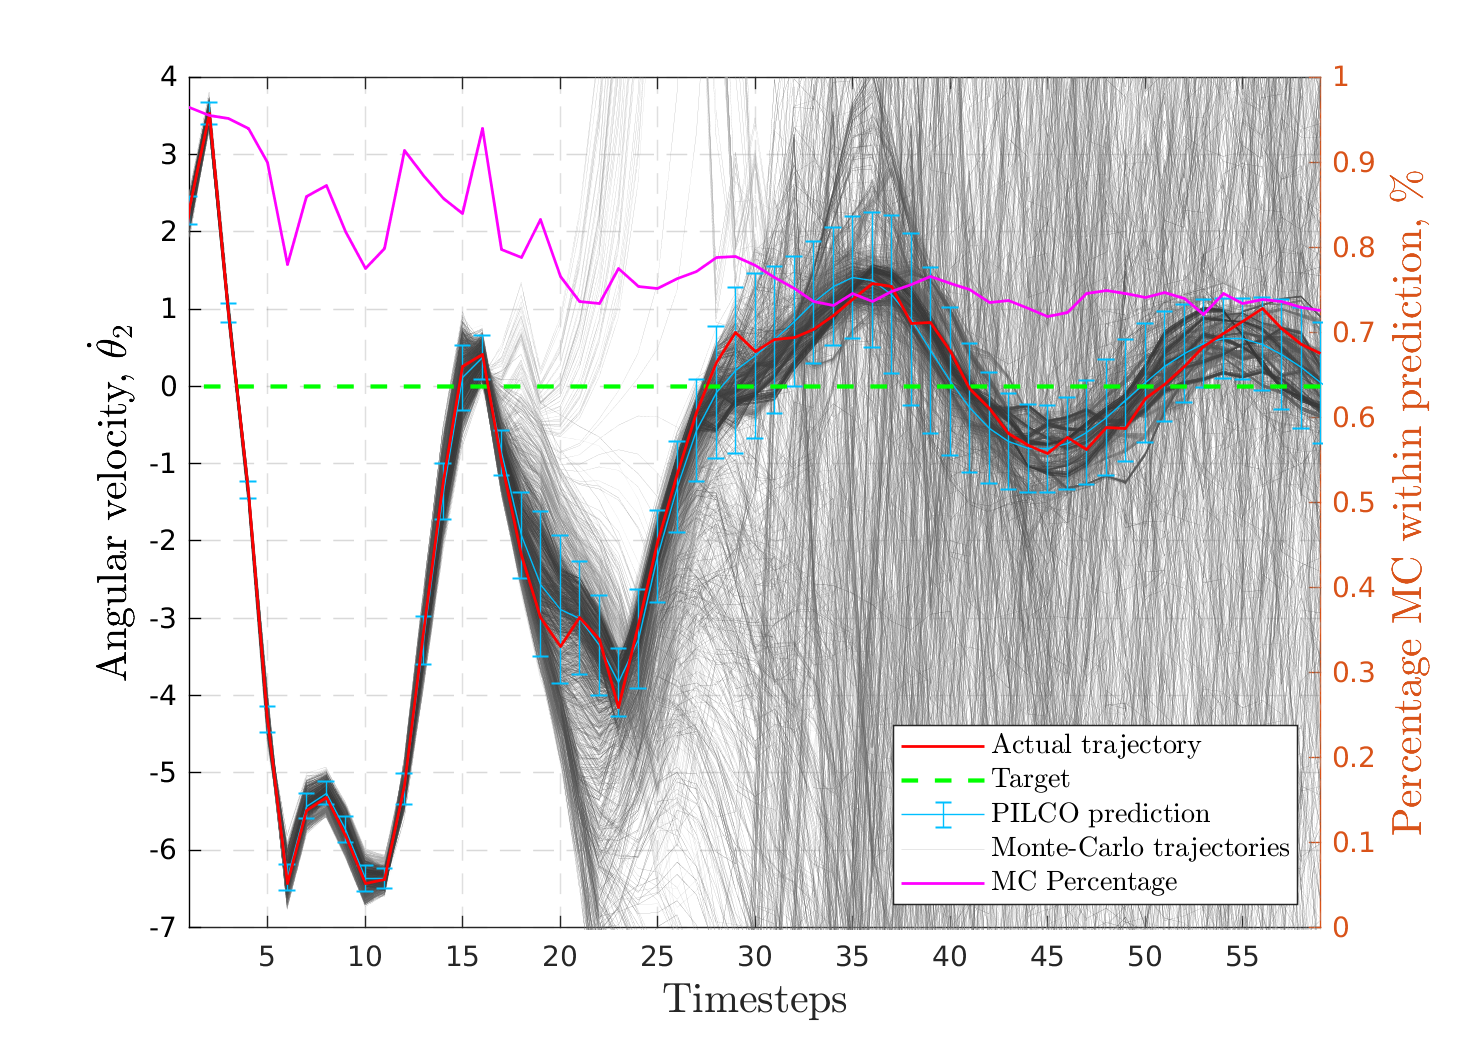
\includegraphics[height=0.4\textheight,width=1\textwidth]{Chapter3/Figures/pen_MC_rollout_Ep_40_Dim_1.png} 
    \caption{Pendulum angular velocity $\dot \theta_{2}$ (rad/s)} 
    \label{Fig:Re-pen-cart-position} 
  \end{subfigure} 
  \hspace{\fill}  %% maximize space between adjacent subfigures
  \begin{subfigure}[b]{1\linewidth}
    \centering
    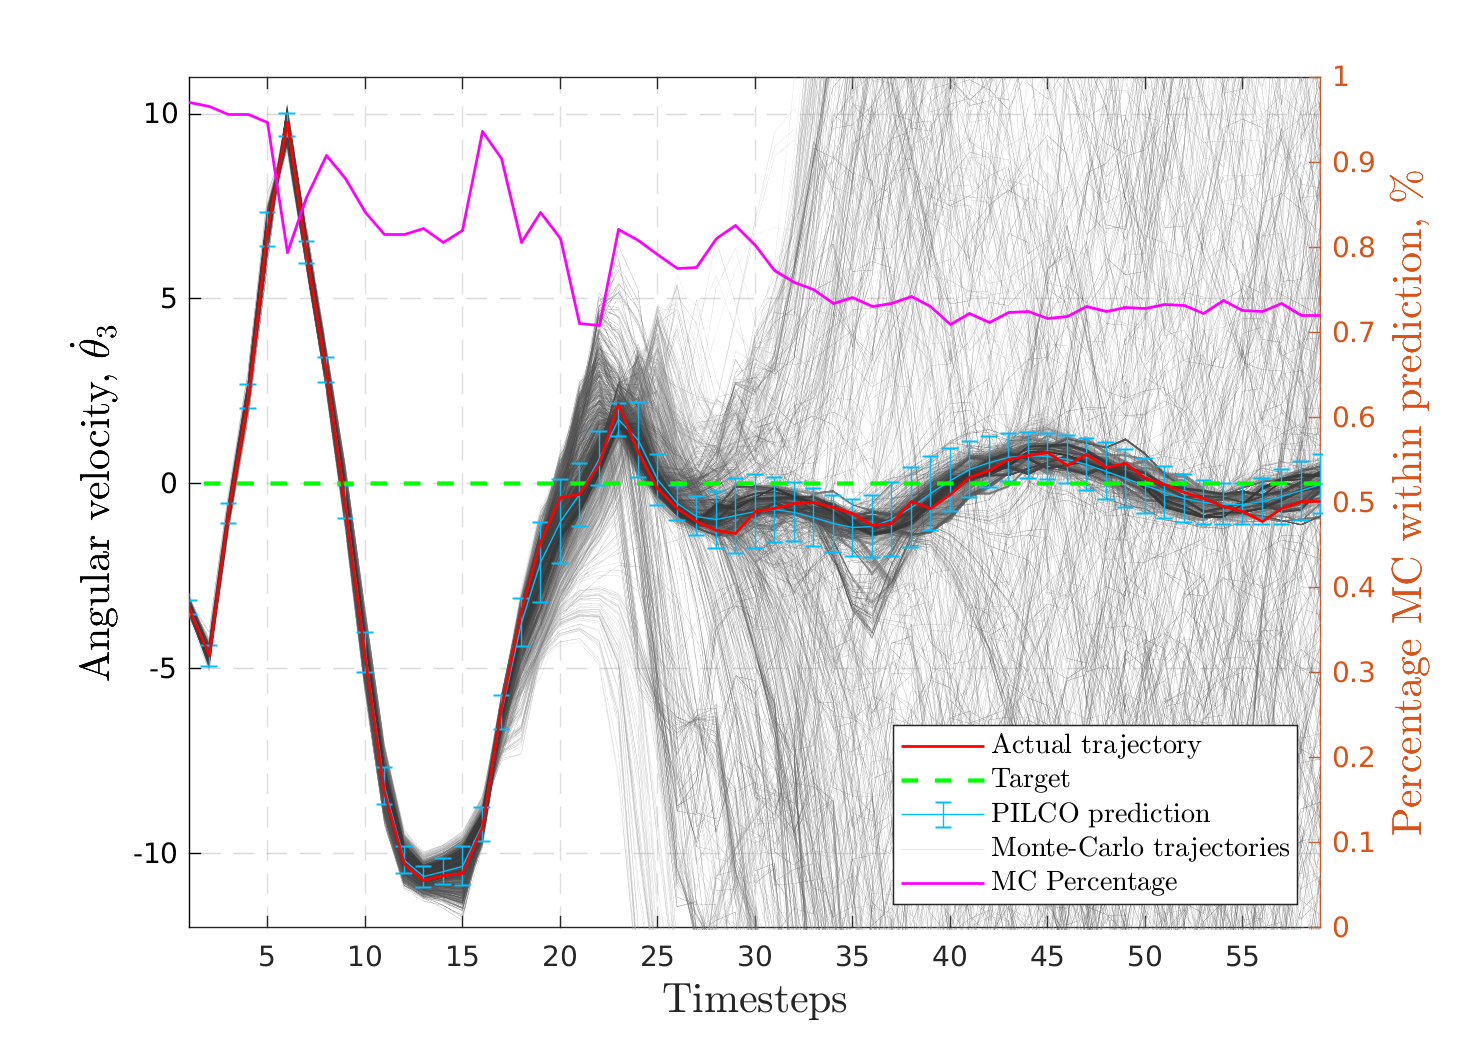
\includegraphics[height=0.4\textheight,width=1\textwidth]{Chapter3/Figures/pen_MC_rollout_Ep_40_Dim_2.png} 
    \caption{Pendulum angular velocity $\dot \theta_{3}$ (rad/s)} 
    \label{Fig:Re-pen-cart-velocity} 
  \end{subfigure} 
\caption[Monte-Carlo roll outs for \textbf{pendubot} pendulum angular velocities]{Monte-Carlo roll outs for the \textbf{pendubot} environment for pendulum angular velocities. Figures show a random sample of the Monte-Carlo trajectories for episode 20. The first three legend items (actual trajectory, target, PILCO prediction and MC trajectories) correspond to the state variable axis (left axis) and the magenta line shows the percentage of MC trajectories inside PILCO's prediction (2 standard deviations) (right axis). Sample time 0.05s, roll out horizon 3.0s.}
\label{Fig:Re-pen-MC-roll-outs-1} 
\end{figure}
 
 
\begin{figure}[htp!]    
   \begin{subfigure}[b]{1\linewidth}
    \centering
    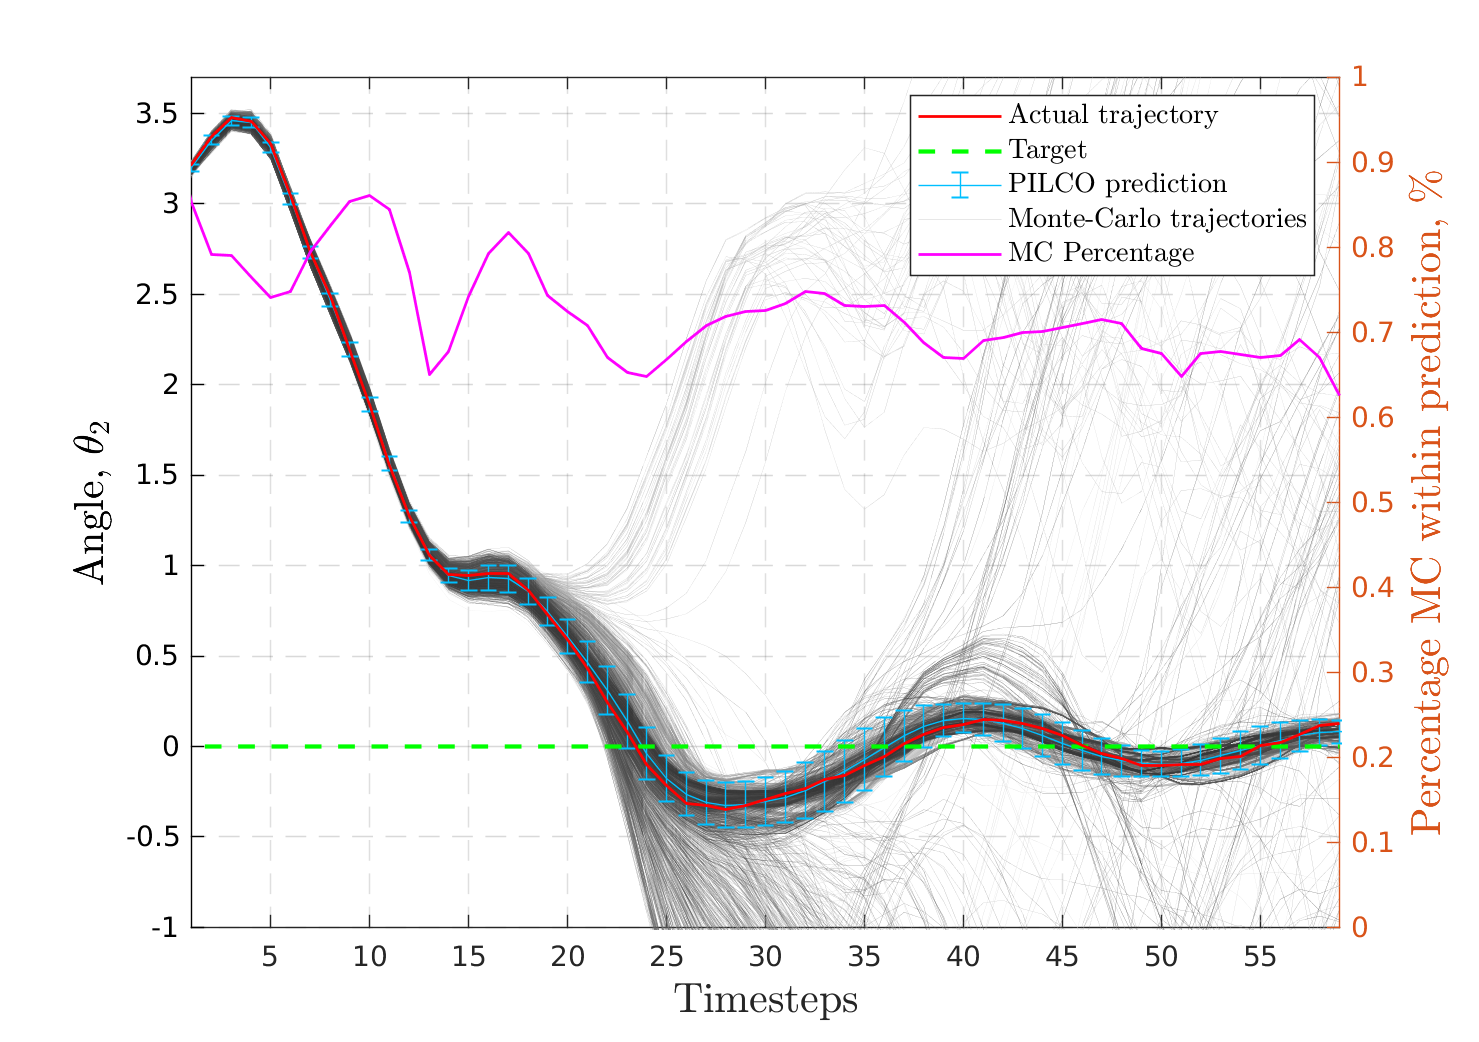
\includegraphics[height=0.4\textheight,width=1\textwidth]{Chapter3/Figures/pen_MC_rollout_Ep_40_Dim_3.png} 
    \caption{Pendulum angle $\theta_2$ (rad)} 
    \label{Fig:Re-pen-pen-velocity} 
  \end{subfigure} 
  \hspace{\fill}
  \begin{subfigure}[b]{1\linewidth}
    \centering
    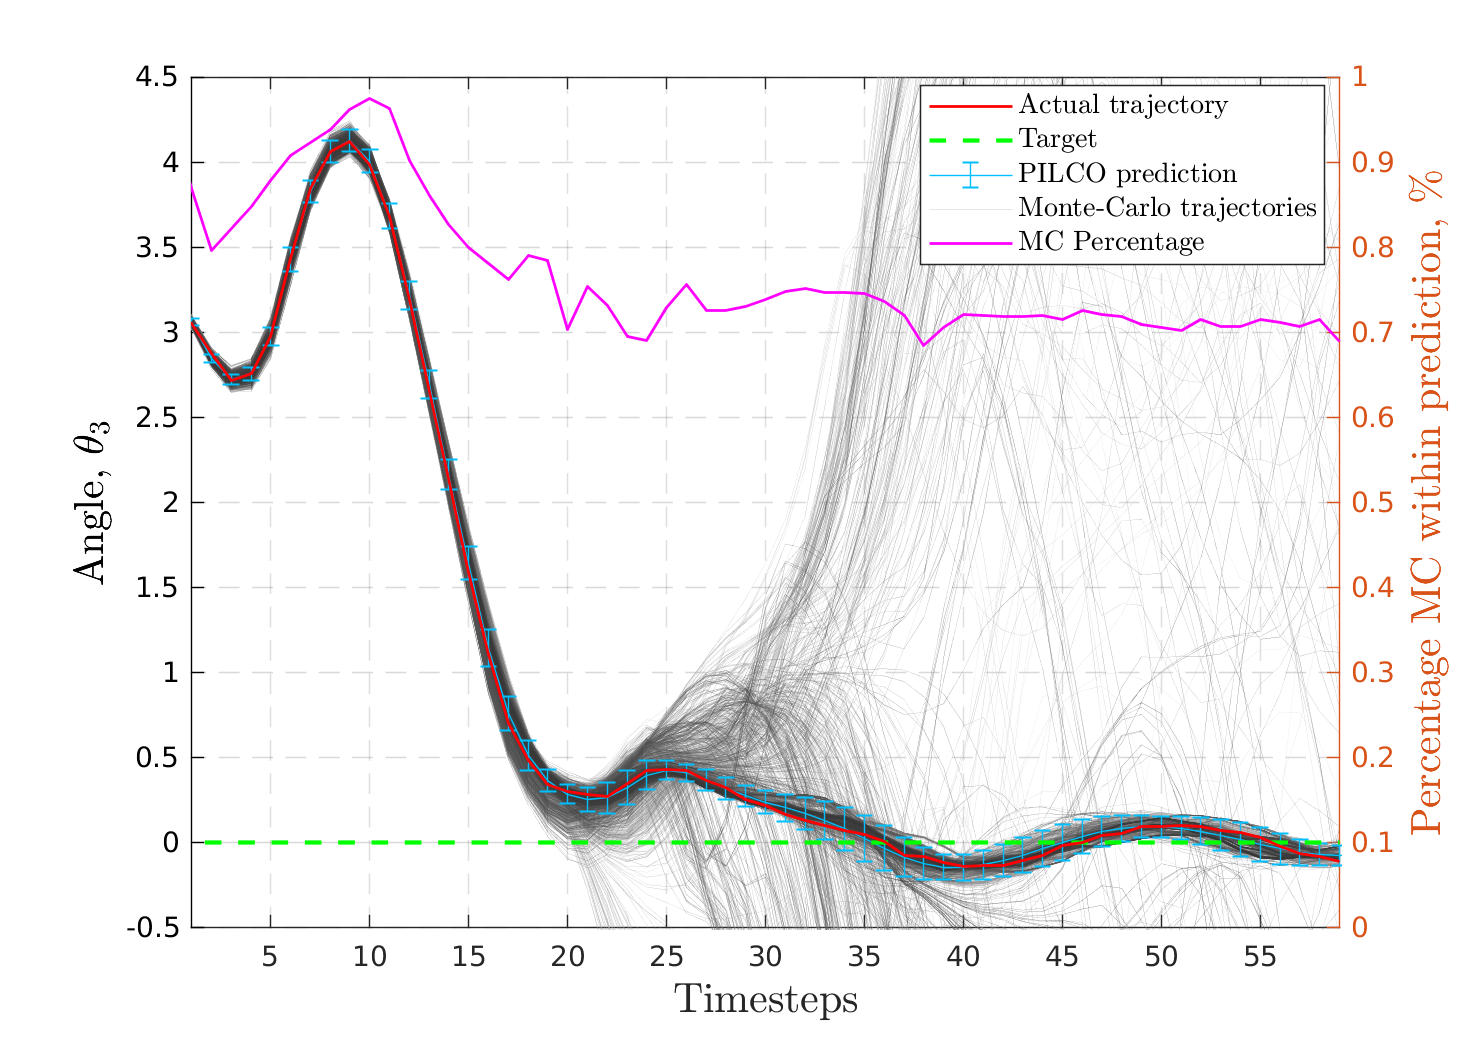
\includegraphics[height=0.4\textheight,width=1\textwidth]{Chapter3/Figures/pen_MC_rollout_Ep_40_Dim_4.png} 
    \caption{Pendulum angle $\theta_3$ (rad)} 
    \label{Fig:Re-pen-pen-angle} 
  \end{subfigure} 

\caption[Monte-Carlo roll outs for \textbf{pendubot} pendulum angles]{Monte-Carlo roll outs for the \textbf{pendubot} environment for pendulum angles. Figures show a random sample of the Monte-Carlo trajectories for episode 20. The first three legend items (actual trajectory, target, PILCO prediction and MC trajectories) correspond to the state variable axis (left axis) and the magenta line shows the percentage of MC trajectories inside PILCO's prediction (2 standard deviations) (right axis). Sample time 0.05s, roll out horizon 3.0s.}
\label{Fig:Re-pen-MC-roll-outs-2} 
\end{figure}
 
\begin{figure}[htp!]    
   \begin{subfigure}[b]{1\linewidth}
    \centering
    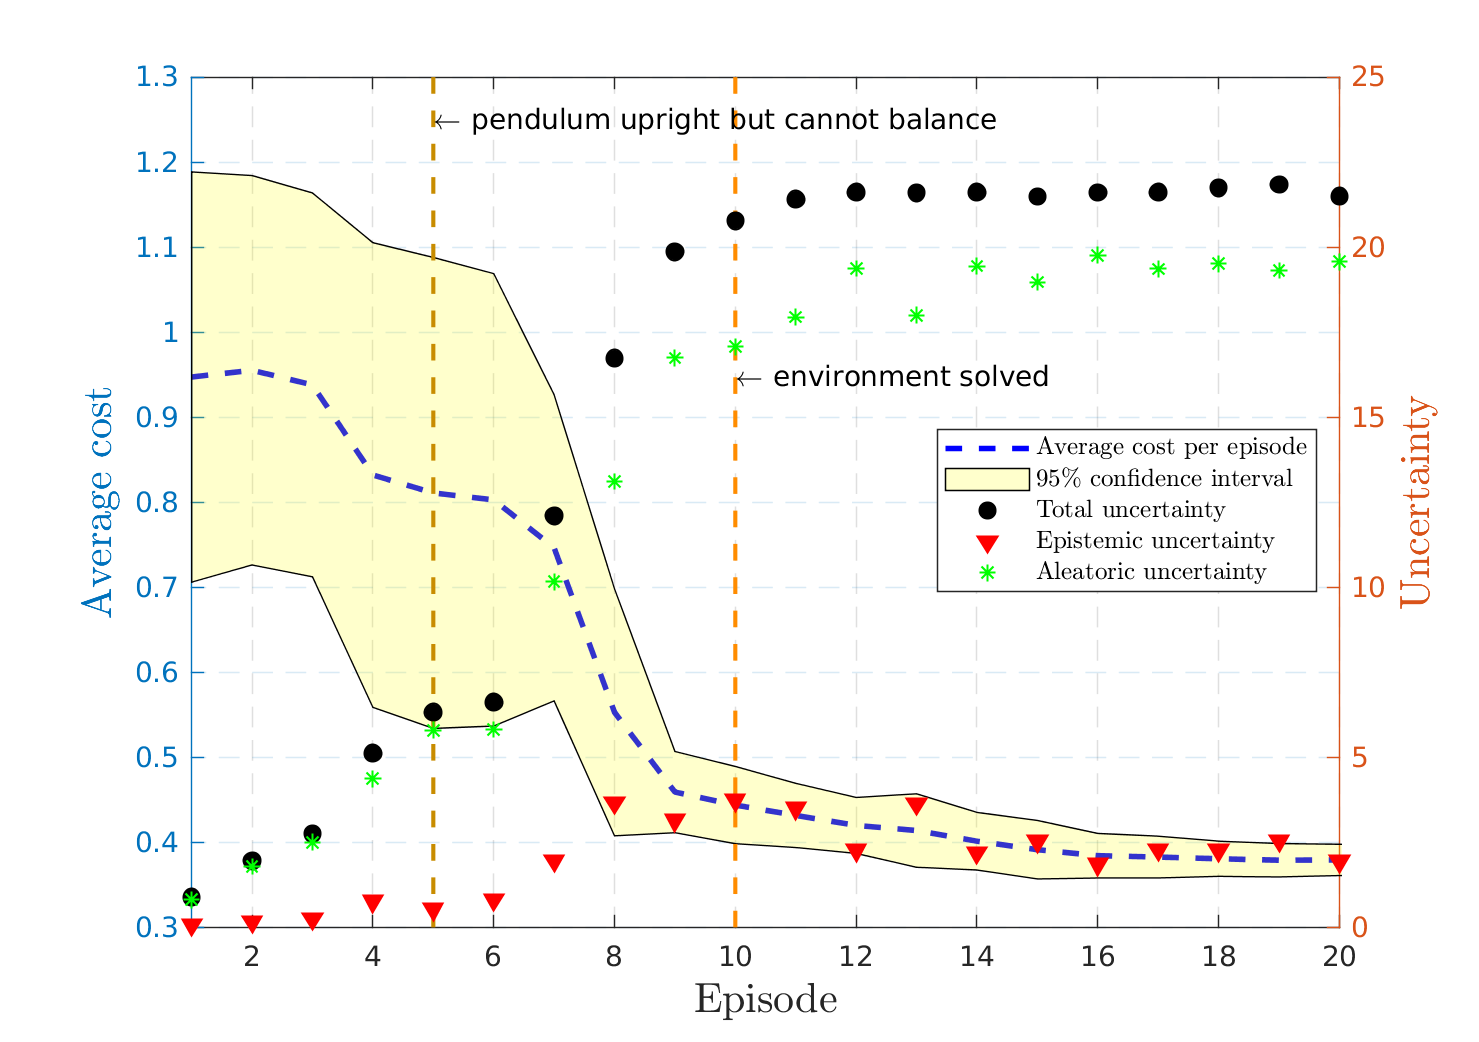
\includegraphics[height=0.4\textheight,width=1\textwidth]{Chapter3/Figures/pen_uncertainty.png} 
    \caption{Average cost (left axis) and uncertainty decomposition (right axis) for each episode over the course of learning.} 
    \label{Fig:Re-pen-uncertainty} 
  \end{subfigure}
  \hspace{\fill}
  \begin{subfigure}[b]{1\linewidth}
    \centering
    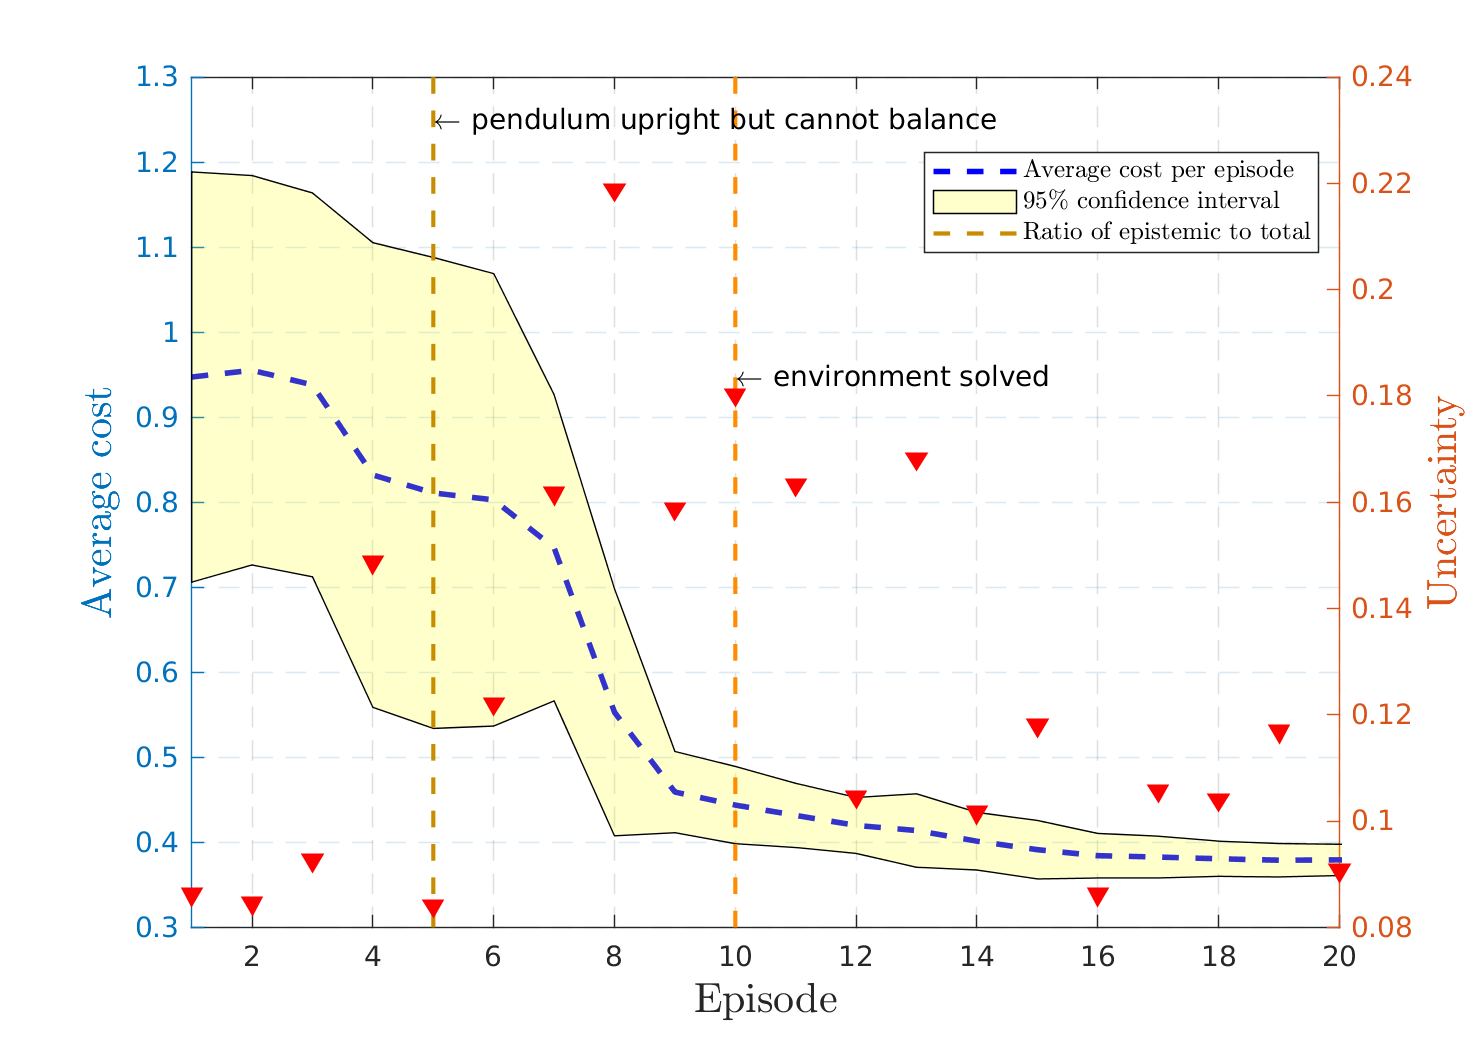
\includegraphics[height=0.4\textheight,width=1\textwidth]{Chapter3/Figures/pen_uncertainty_norm.png} 
    \caption{Average cost (left axis) and ratio of epistemic to total uncertainty (right axis) for each episode over the course of learning.} 
    \label{Fig:Re-pen-uncertainty-norm} 
  \end{subfigure} 
\caption[Uncertainty decomposition for \textbf{pendubot} environment]{\textbf{Pendubot}: Average cost (left axis) and uncertainty (right axis) for each episode over the course of learning.}
\label{Fig:Re-pen-full-uncertainty} 
\end{figure}


\subsubsection{Cart-Double-Pendulum}
Fig. \ref{Fig:Re-cdp-MC-roll-outs-1} - \ref{Fig:Re-cdp-MC-roll-outs-3} show a random sample of the Monte-Carlo trajectory roll outs for the state variables of the cart-double-pendulum environment: cart position $x$, cart velocity $\dot x$, pendulum angular velocities $\dot{\theta}_{2}$, $\dot{\theta}_{3}$ and pendulum angles $\theta_{2}$, $\theta_{3}$. The trajectories shown in the figures are from episode 80, when PILCO has achieved the environment objective, and so represent trajectories under a mature policy $\pi$. Up to approximately 30 time steps there is cohesion in the Monte-Carlo trajectories which again corresponds to the swing-up phase. During the balance phase, the trajectories spread out. By the end of the episode, only about $40\%$ of the trajectories fall within PILCO's predictions. 

Fig. \ref{Fig:Re-cdp-full-uncertainty} shows the average cost per episode and the uncertainty in the cost over the course of learning. Starting with Fig. \ref{Fig:Re-cdp-uncertainty}. After 10 episodes, the agent has learned to swing the pendulums into the upright position but cannot yet maintain them in a balanced state. During this phase there is a small reduction in average cost. The agent then takes a further 33 episodes to learn to maintain the pendulums in a balanced but off-centre position. Remarkably, the act of balancing the pendulums is a significantly harder problem to solve than swinging them into position. During this second phase of learning, the total and epistemic cost uncertainties increase as the agent forms a belief about the environment, however, policies associated with low epistemic cost uncertainty are consistently being selected. Consequently, the learning gradient is gentle. Just after 40 episodes, there is a rapid increase in learning. During this phase, the total cost uncertainty rises further and departs from the trend  of the aleatoric cost uncertainty due to the increase in epistemic cost uncertainty. 

Fig. \ref{Fig:Re-cdp-uncertainty-normalised} shows a more pronounced trend in the ratio of total to epistemic cost uncertainty. Approaching the 40 episode mark, PILCO selects policies with an increasing ratio of total to epistemic cost uncertainty and as a consequence learning increases. Here there is a clear correlation between the amount of epistemic cost uncertainty present in the policy and the average cost. This shows that policies with a high epistemic cost uncertainty lead to a steeper learning gradient. 

 \begin{figure}[H]    
    \begin{subfigure}[b]{1\linewidth}
    \centering
    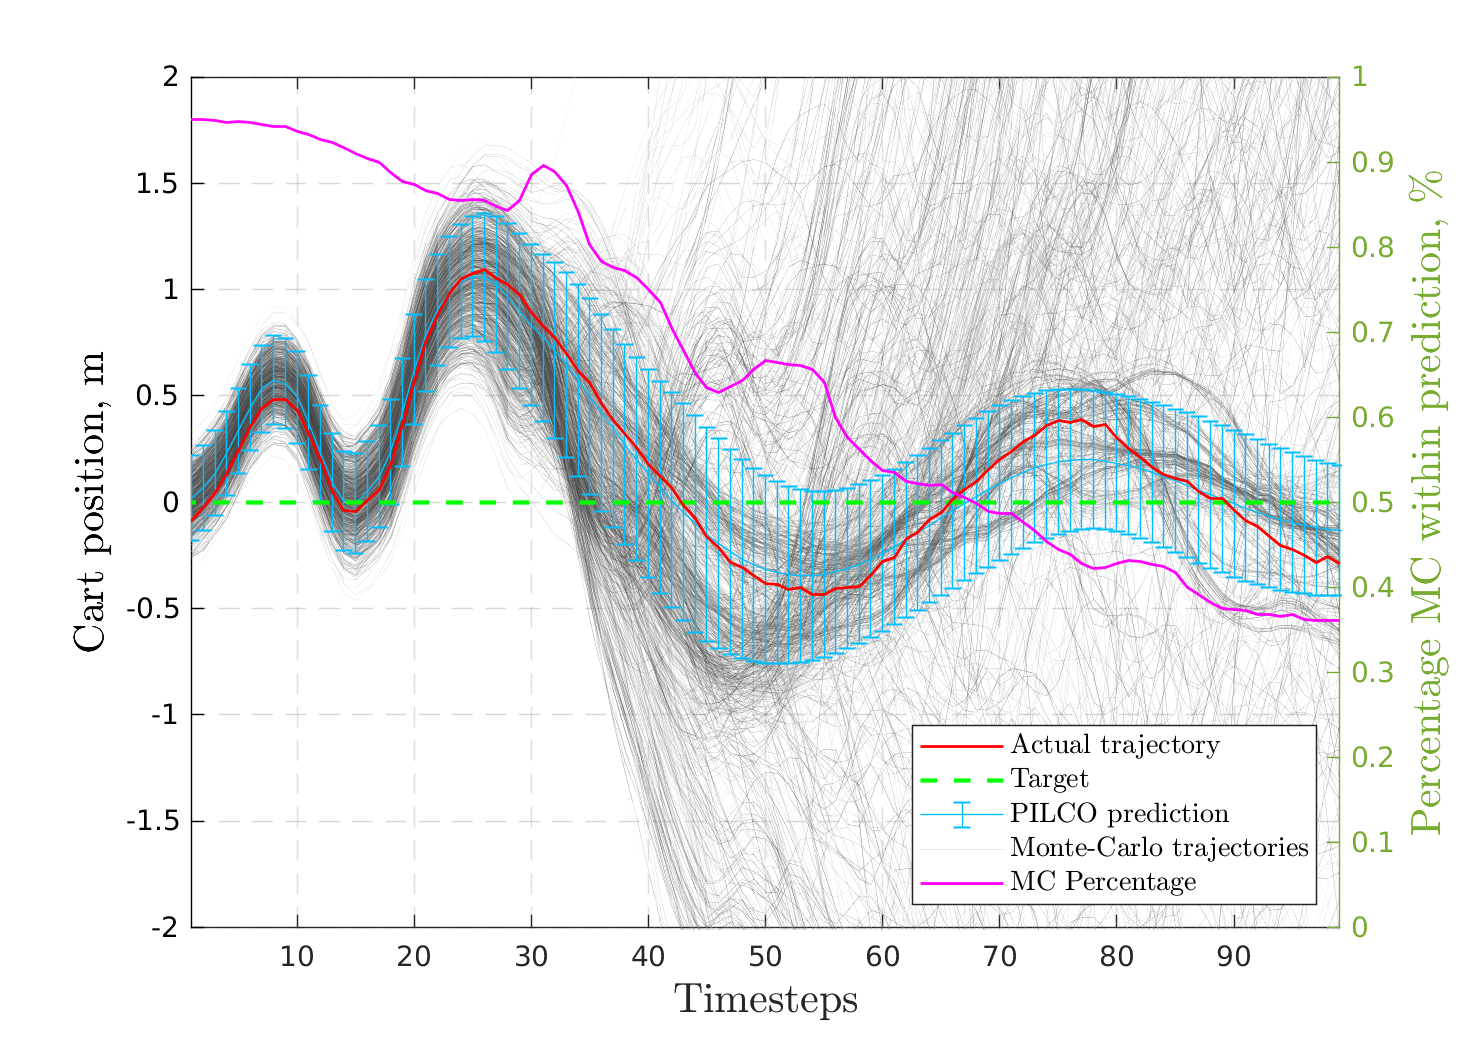
\includegraphics[height=0.4\textheight,width=1\textwidth]{Chapter3/Figures/cdp_MC_rollout_Ep_80_Dim_1.png} 
    \caption{Cart position $x_1$ (m)} 
    \label{Fig:Re-cdp-cart-position} 
  \end{subfigure} 

  \begin{subfigure}[b]{1\linewidth}
    \centering
    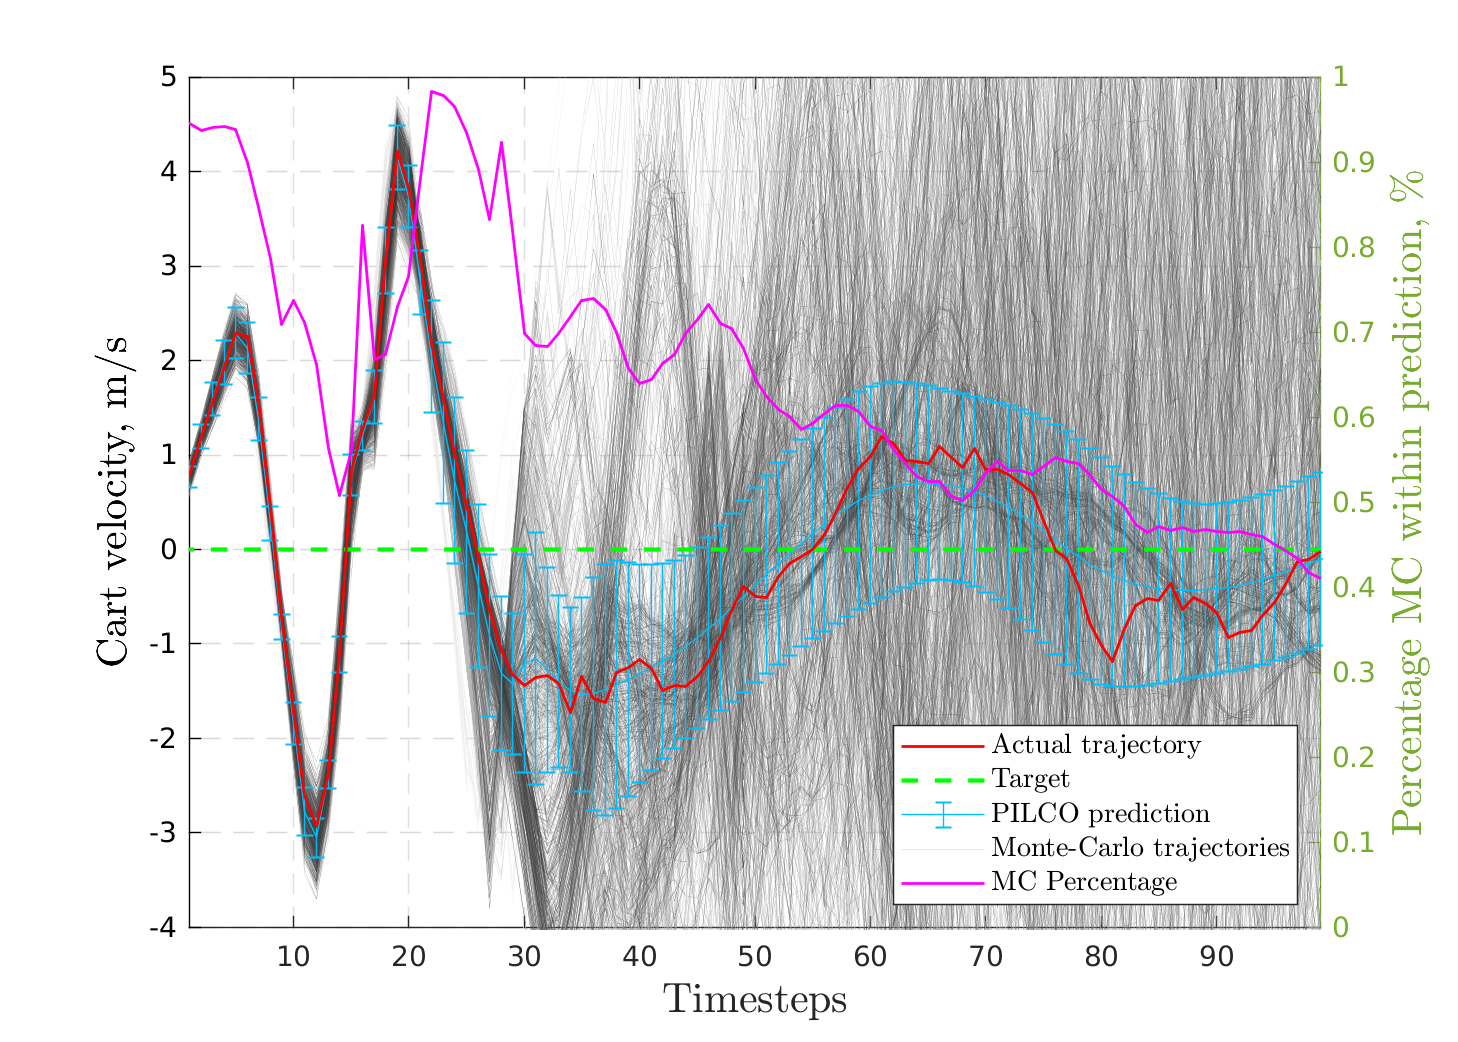
\includegraphics[height=0.4\textheight,width=1\textwidth]{Chapter3/Figures/cdp_MC_rollout_Ep_80_Dim_2.png} 
    \caption{Cart velocity $\dot{x}_1$ (m/s)} 
    \label{Fig:Re-cdp-cart-velocity} 
  \end{subfigure} 
\caption[Monte-Carlo roll outs for \textbf{cart-double-pendulum} cart position and cart velocity]{Monte-Carlo roll outs for the \textbf{cart-double-pendulum} environment for cart position and cart velocity. Figures show a random sample of the Monte-Carlo trajectories for episode 75. The first three legend items (actual trajectory, target, PILCO prediction and MC trajectories) correspond to the state variable axis (left axis) and the magenta line shows the percentage of MC trajectories inside PILCO's prediction (2 standard deviations) (right axis). Sample time 0.05s, roll out horizon 5.0s.}
\label{Fig:Re-cdp-MC-roll-outs-1} 
\end{figure}
 
 
\begin{figure}[H]    
   \begin{subfigure}[b]{1\linewidth}
    \centering
    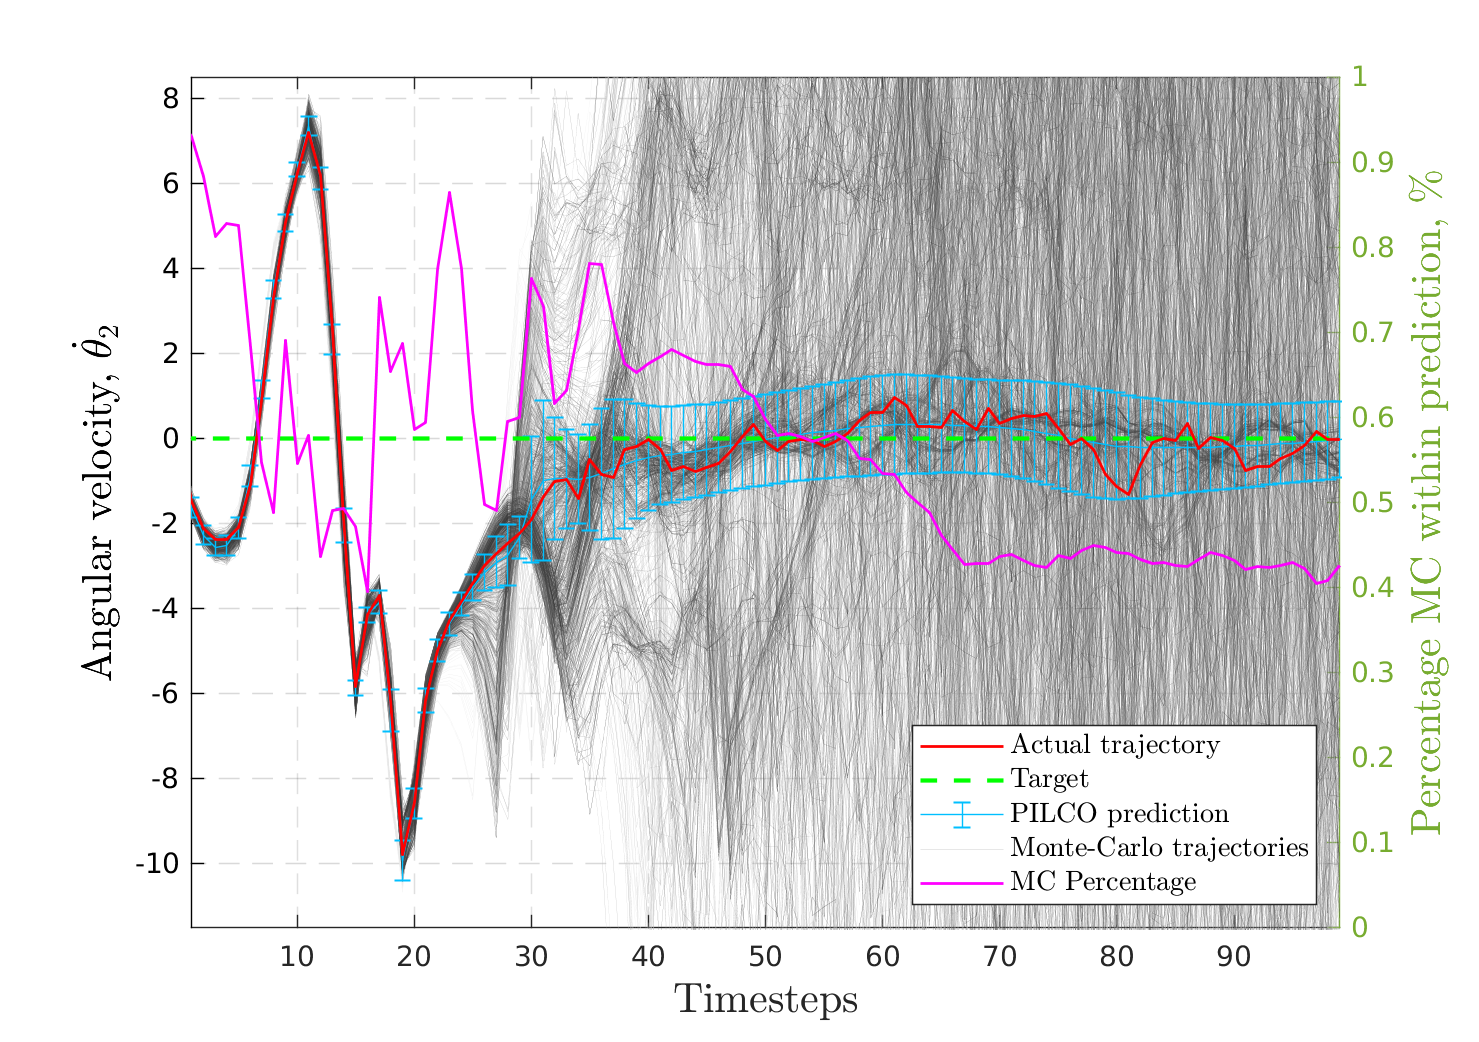
\includegraphics[height=0.4\textheight,width=1\textwidth]{Chapter3/Figures/cdp_MC_rollout_Ep_80_Dim_3.png} 
    \caption{Pendulum angular velocity $\dot{\theta}_2$ (rad/s)} 
    \label{Fig:Re-cdp-pen2-velocity} 
  \end{subfigure} 
  \hspace{\fill}
  \begin{subfigure}[b]{1\linewidth}
    \centering
    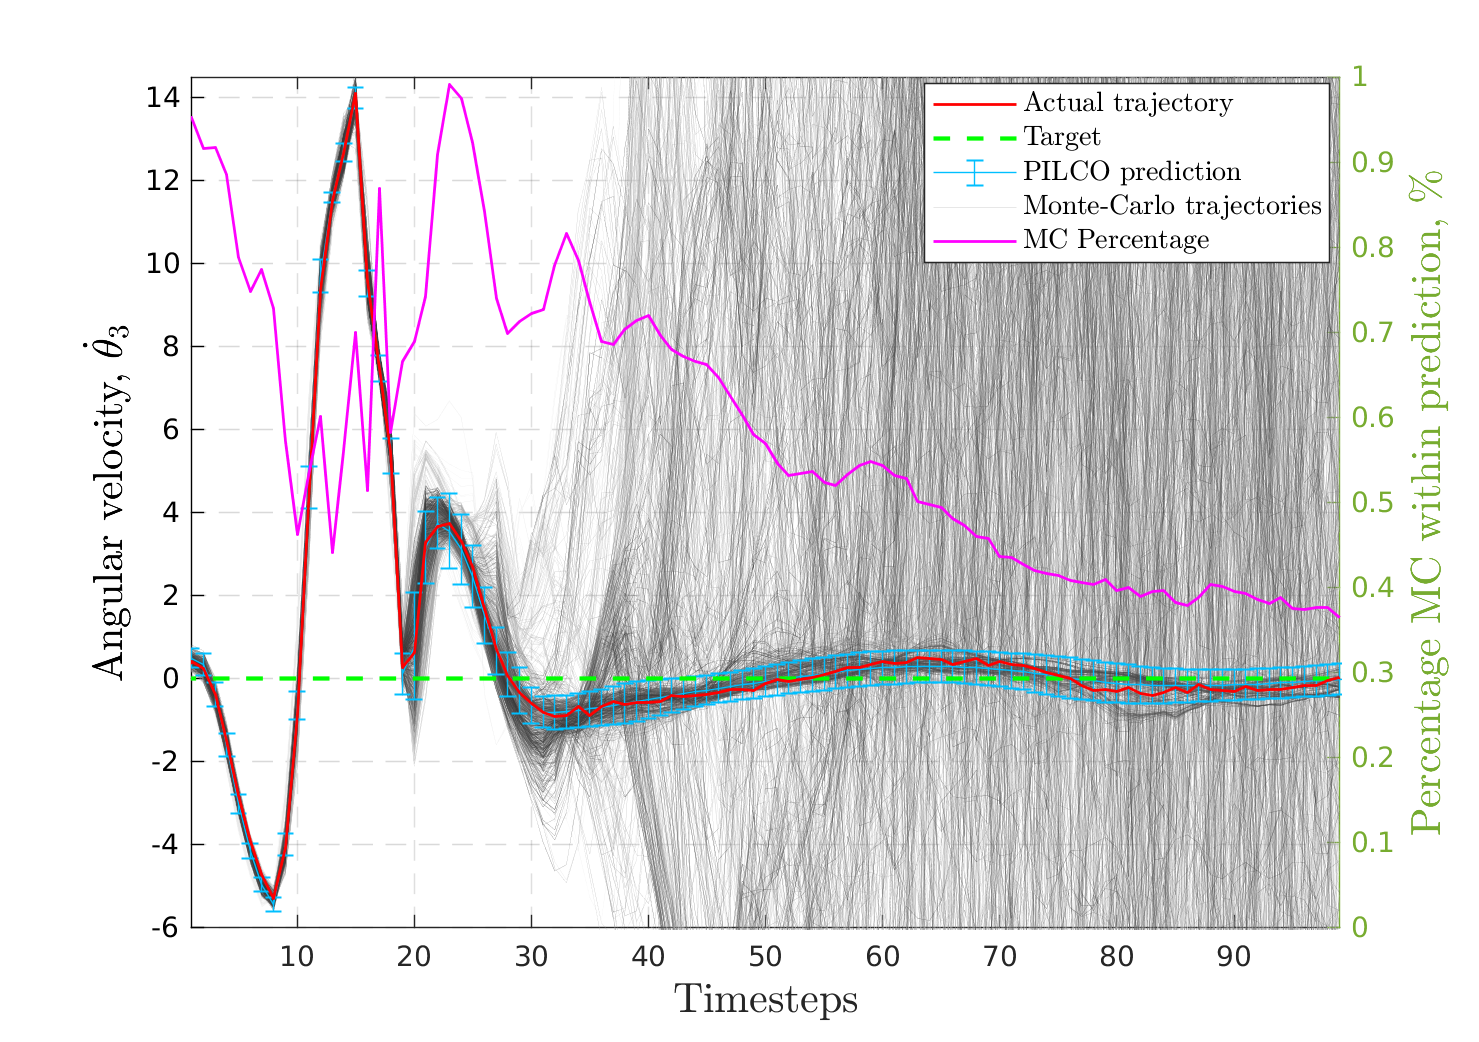
\includegraphics[height=0.4\textheight,width=1\textwidth]{Chapter3/Figures/cdp_MC_rollout_Ep_80_Dim_4.png} 
    \caption{Pendulum angular velocity $\dot{\theta}_3$ (rad/s)} 
    \label{Fig:Re-cdp-pen3-velocity} 
  \end{subfigure} 

\caption[Monte-Carlo roll outs for \textbf{cart-double-pendulum} pendulum angular velocities]{Monte-Carlo roll outs for the \textbf{cart-double-pendulum} environment for  pendulum angular velocities]. Figures show a random sample of the Monte-Carlo trajectories for episode 75. The first three legend items (actual trajectory, target, PILCO prediction and MC trajectories) correspond to the state variable axis (left axis) and the magenta line shows the percentage of MC trajectories inside PILCO's prediction (2 standard deviations) (right axis). Sample time 0.05s, roll out horizon 5.0s.}
\label{Fig:Re-cdp-MC-roll-outs-2} 
\end{figure}
 
\begin{figure}[H]    
    \begin{subfigure}[b]{1\linewidth}
    \centering
    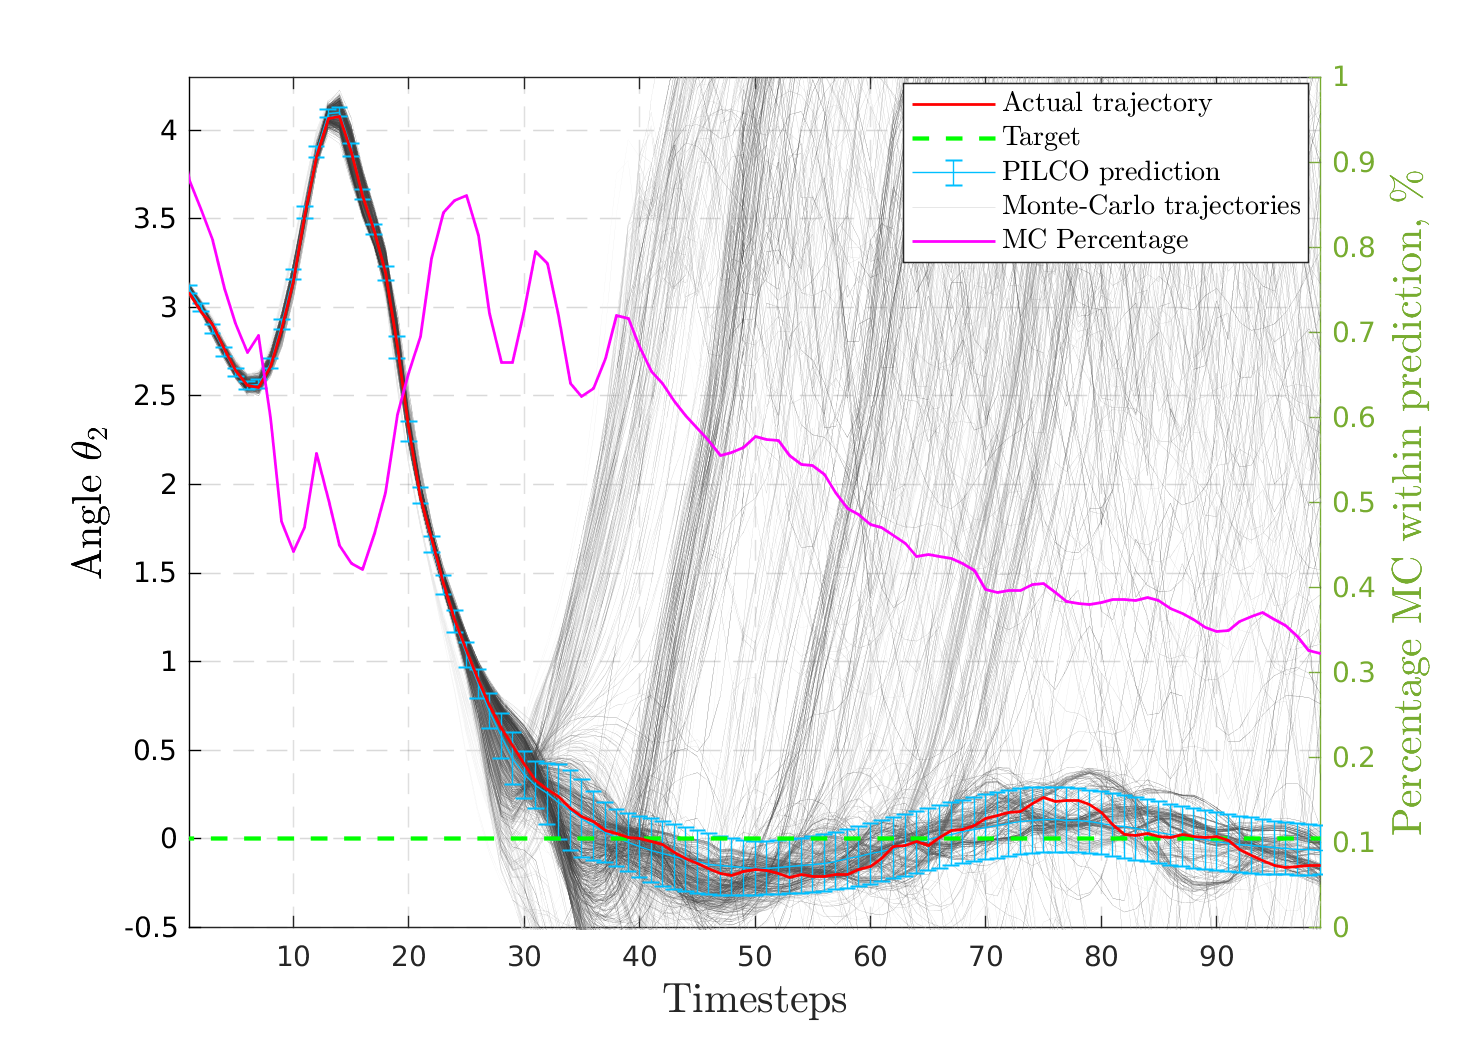
\includegraphics[height=0.4\textheight,width=1\textwidth]{Chapter3/Figures/cdp_MC_rollout_Ep_80_Dim_5.png} 
    \caption{Pendulum angle $\theta_2$ (rad)} 
    \label{Fig:Re-cdp-angle2} 
  \end{subfigure}
  \hspace{\fill}
  \begin{subfigure}[b]{1\linewidth}
    \centering
    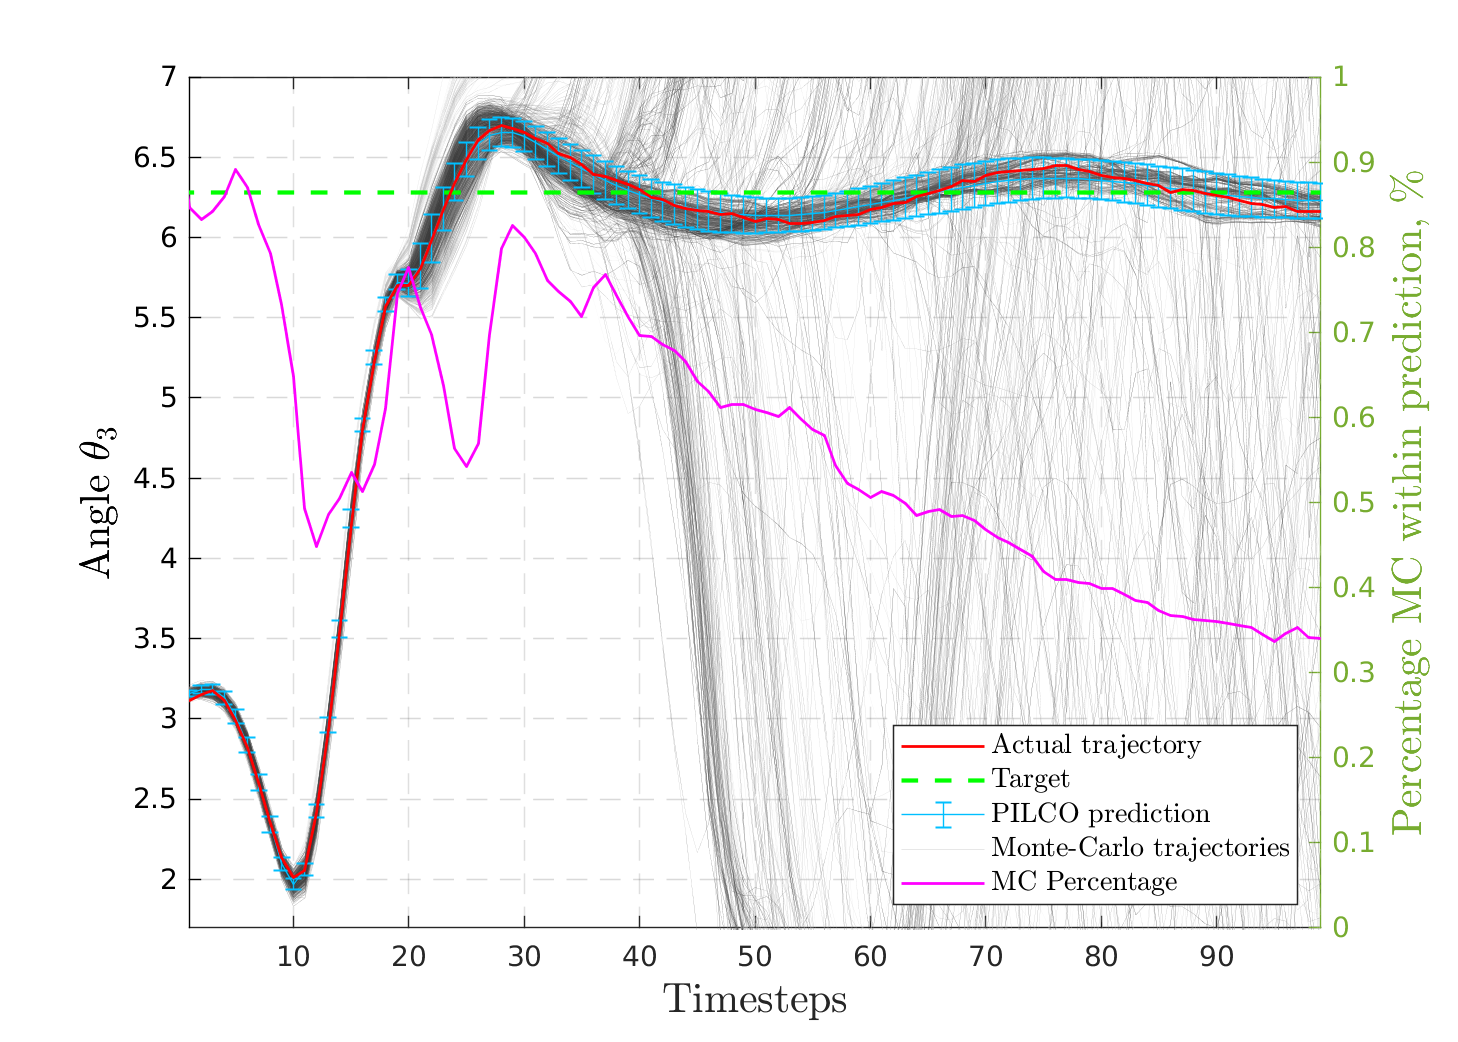
\includegraphics[height=0.4\textheight,width=1\textwidth]{Chapter3/Figures/cdp_MC_rollout_Ep_80_Dim_6.png} 
    \caption{Pendulum angle $\theta_3$ (rad)} 
    \label{Fig:Re-cdp-angle3} 
  \end{subfigure} 
\caption[Monte-Carlo roll outs for \textbf{cart-double-pendulum} pendulum angles]{Monte-Carlo roll outs for the \textbf{cart-double-pendulum} environment for  pendulum angles]. Figures show a random sample of the Monte-Carlo trajectories for episode 75. The first three legend items (actual trajectory, target, PILCO prediction and MC trajectories) correspond to the state variable axis (left axis) and the magenta line shows the percentage of MC trajectories inside PILCO's prediction (2 standard deviations) (right axis). Sample time 0.05s, roll out horizon 5.0s.}
\label{Fig:Re-cdp-MC-roll-outs-3} 
\end{figure} 
 
 
\begin{figure}[H]    
  \begin{subfigure}[b]{1\linewidth}
    \centering
    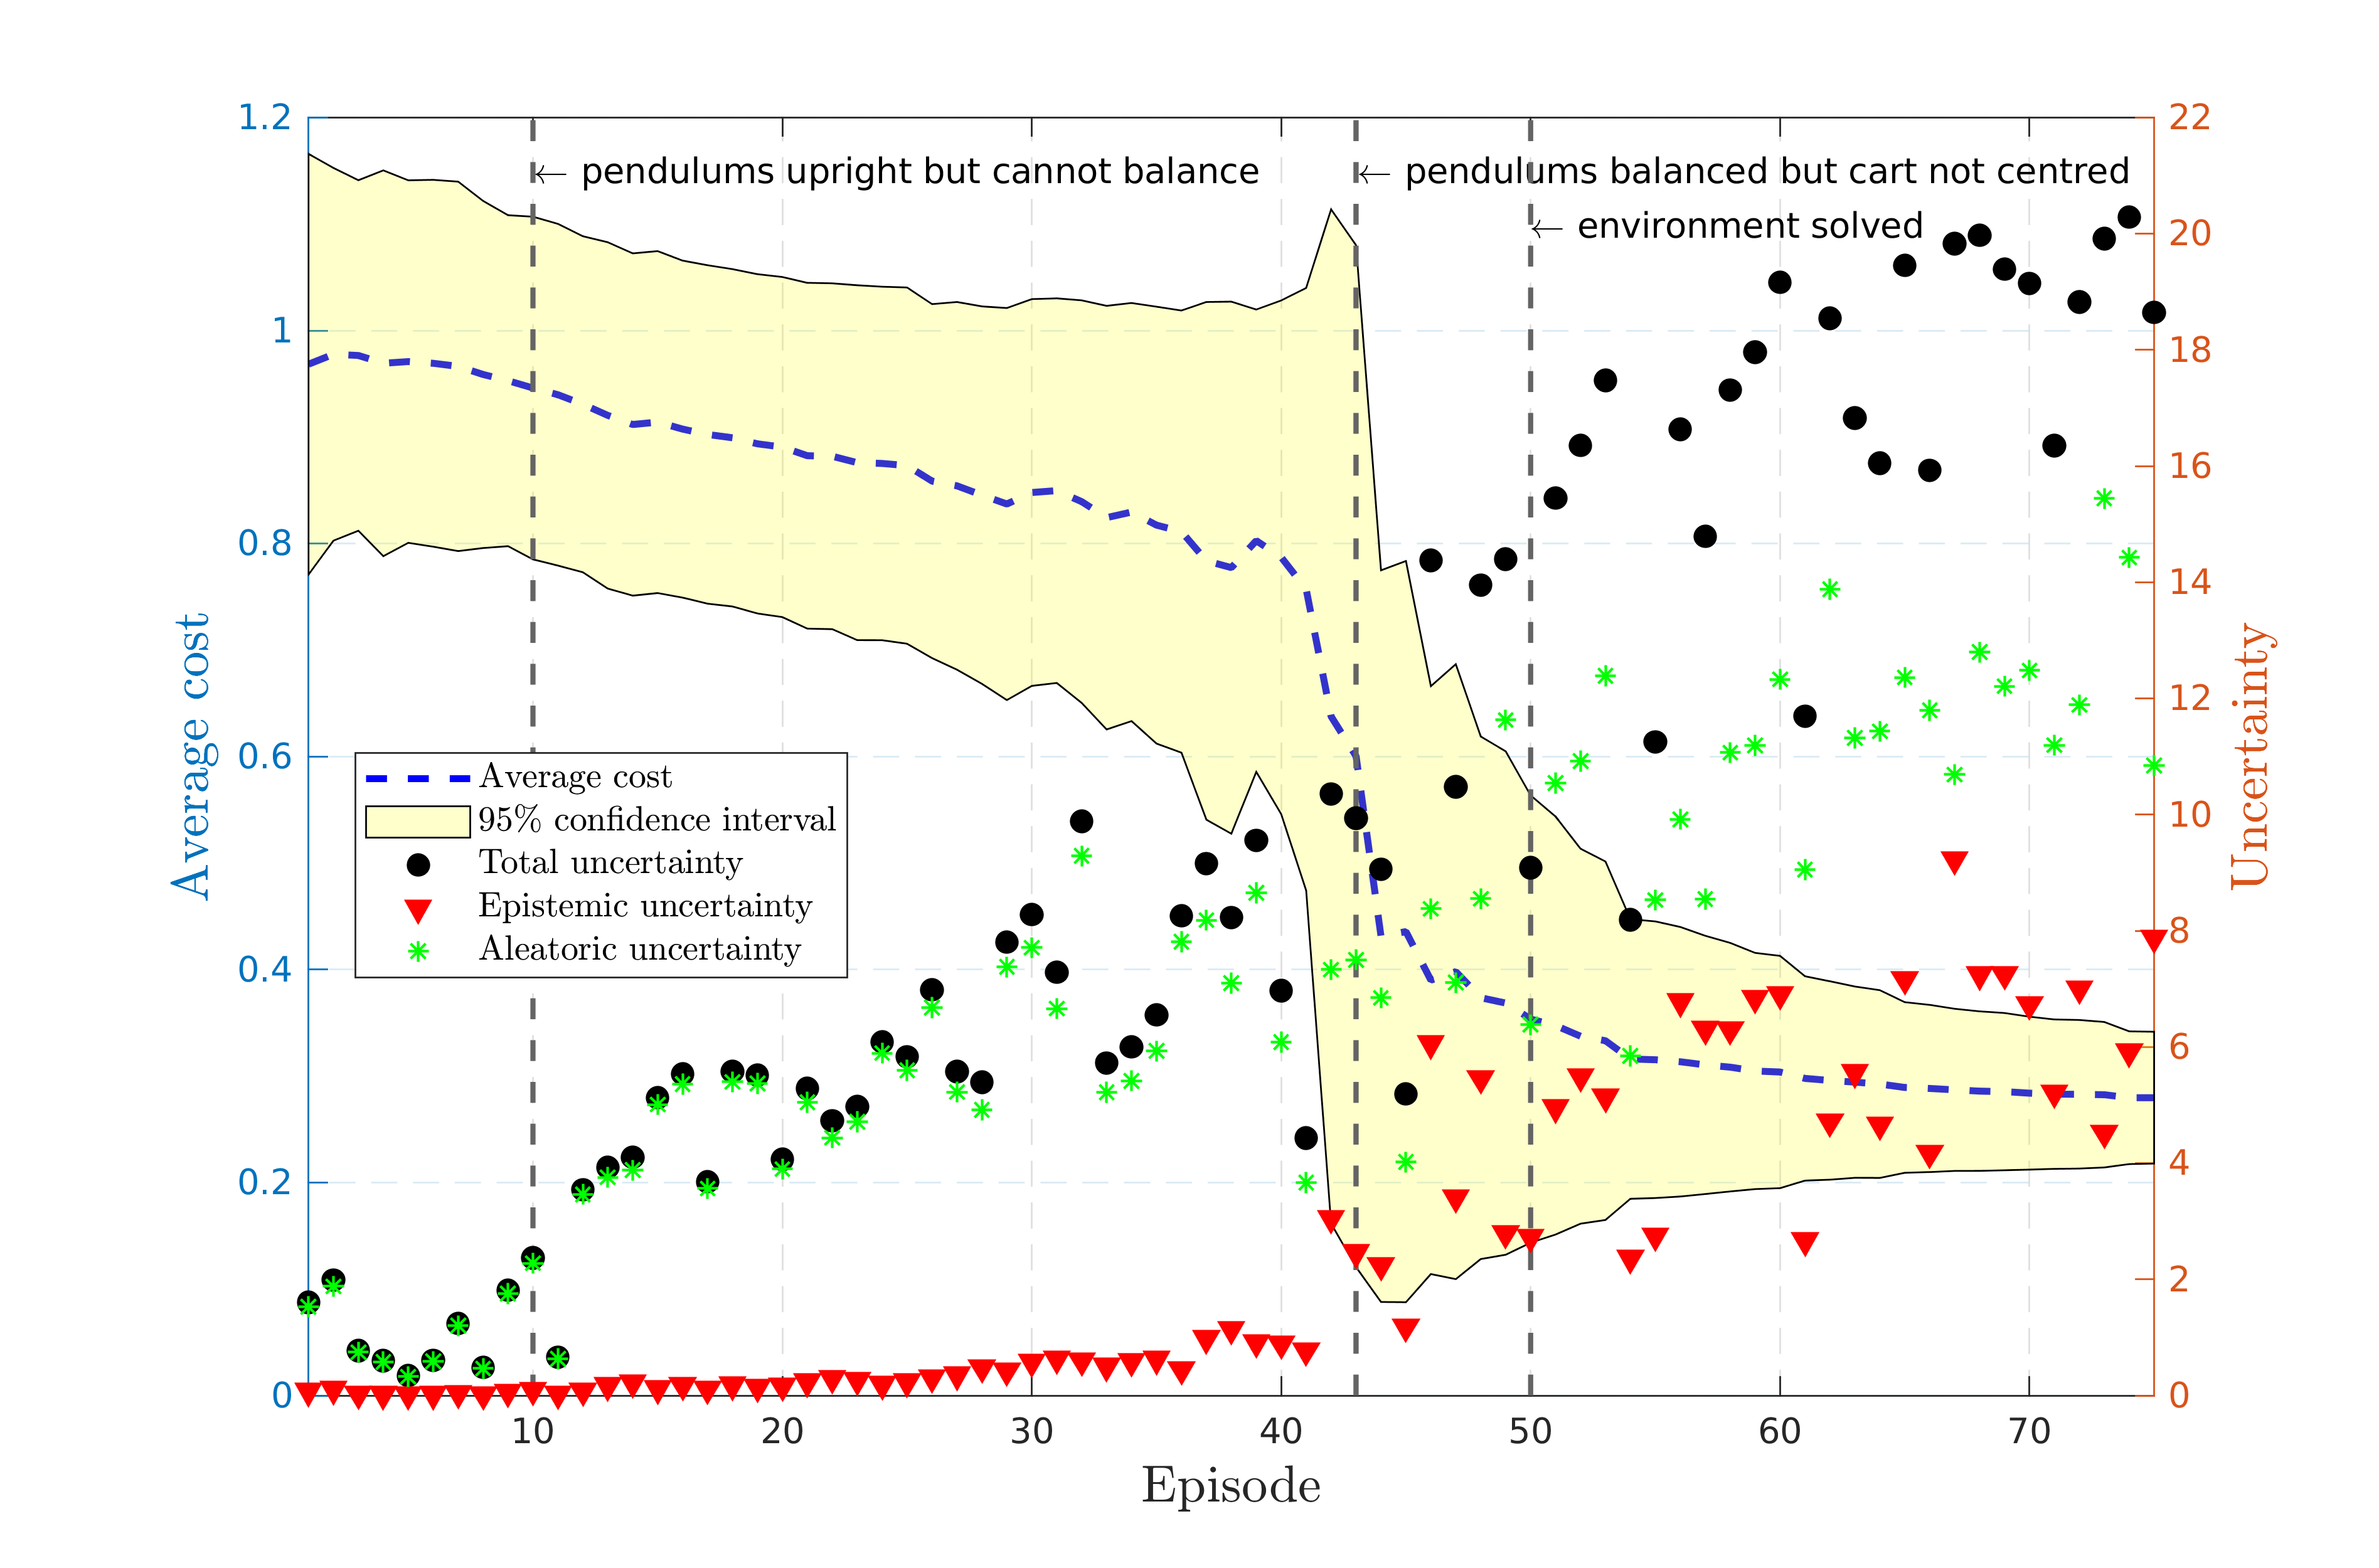
\includegraphics[height=0.4\textheight,width=1\textwidth]{Chapter3/Figures/cdp_uncertainty.png}
    \caption{Average cost (left axis) and uncertainty decomposition (right axis) for each episode over the course of learning.} 
    \label{Fig:Re-cdp-uncertainty} 
  \end{subfigure} 
  \begin{subfigure}[b]{1\linewidth}
    \centering
    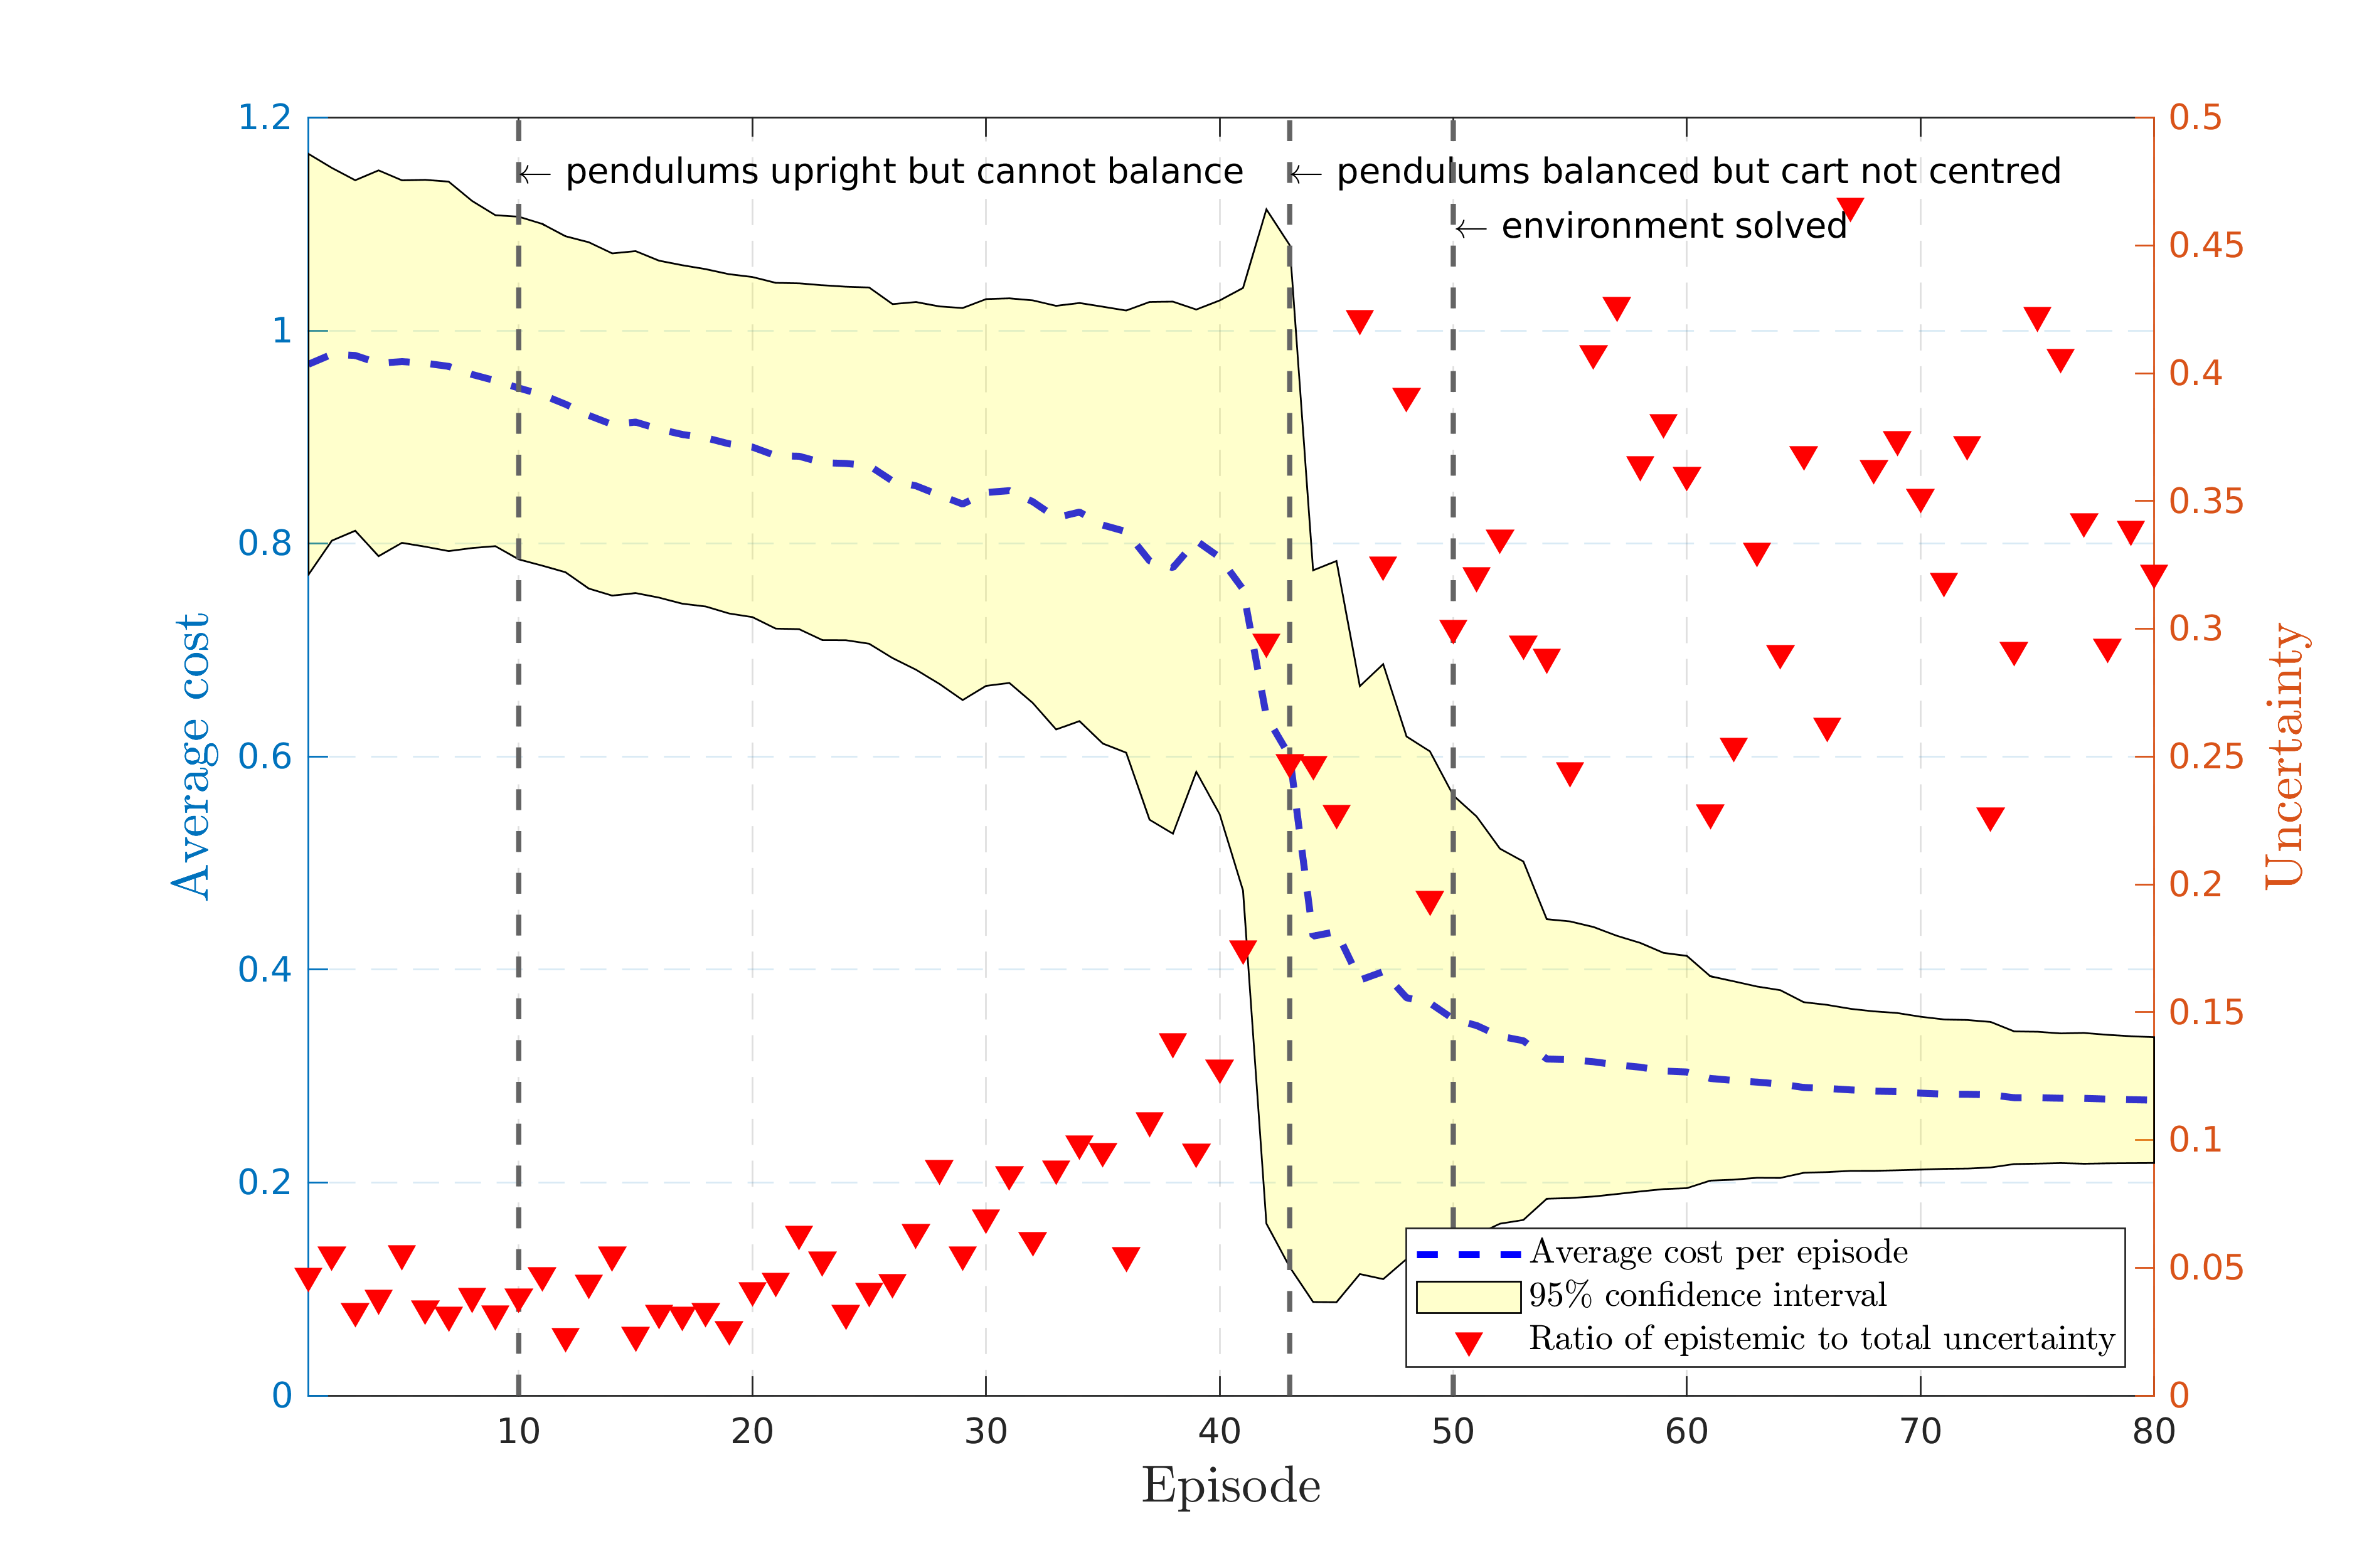
\includegraphics[height=0.4\textheight,width=1\textwidth]{Chapter3/Figures/cdp_uncertainty_normalised.png} 
    \caption{Average cost (left axis) and ratio of epistemic to total uncertainty (right axis) for each episode over the course of learning.} 
    \label{Fig:Re-cdp-uncertainty-normalised} 
  \end{subfigure} 
\caption[Uncertainty decomposition for \textbf{cart-double-pole} environment]{\textbf{Cart-double-pole}: Average cost (left axis) and uncertainty (right axis) for each episode over the course of learning.}
\label{Fig:Re-cdp-full-uncertainty} 
\end{figure}

\section{Discussion}
Discussion:
During this second phase of learning, the total and epistemic cost uncertainties increase as the agent forms a belief about the environment but is consistently selecting policies associated with low epistemic cost uncertainty. This is indicative of both PILCO's purely exploitative policy and the its tendency to favour uncertain states makes the learning creep forward.

Should more episodes be run one would then expect the epistemic cost uncertainty to decrease as the agents belief becomes more confident. And then again increase because of favour towards uncertain states.
\section{Conclusion}




%\include{Chapter4/chapter4}
%\include{Chapter5/chapter5}
%\include{Chapter6/chapter6}
%\include{Chapter7/chapter7}



% ********************************** Back Matter *******************************
% Backmatter should be commented out, if you are using appendices after References
%\backmatter

% ********************************** Bibliography ******************************
\begin{spacing}{0.9}

% To use the conventional natbib style referencing
% Bibliography style previews: http://nodonn.tipido.net/bibstyle.php
% Reference styles: http://sites.stat.psu.edu/~surajit/present/bib.htm

\bibliographystyle{apalike}
%\bibliographystyle{unsrt} % Use for unsorted references  
%\bibliographystyle{plainnat} % use this to have URLs listed in References
\cleardoublepage
\bibliography{References/references} % Path to your References.bib file


% If you would like to use BibLaTeX for your references, pass `custombib' as
% an option in the document class. The location of 'reference.bib' should be
% specified in the preamble.tex file in the custombib section.
% Comment out the lines related to natbib above and uncomment the following line.

%\printbibliography[heading=bibintoc, title={References}]


\end{spacing}

% ********************************** Appendices ********************************

\begin{appendices} % Using appendices environment for more functunality

%!TEX root = ../thesis.tex
% ******************************* Thesis Appendix A ****************************
\chapter{Derivations} 

\section{Model}
\subsection{Posterior Distribution}
\label{A:derivation-posterior-over-weights}
The prior distribution over the weights $p(\mathbf{w})$ and the model likelihood $p(\mathbf{y} | \mathbf{X}, \mathbf{w}, \sigma_{n}^{2})$ are 
\begin{equation}
    p\left(\mathbf{w}\right)= \mathcal{N}\left(\mathbf{w} | \mathbf{0}, \frac{\sigma_{0}^{2}}{m}\mathbf{I}\right)
\end{equation}
\begin{equation}
    p\left(\mathbf{y} | \mathbf{X}, \mathbf{w}, \sigma_{n}^{2}\right)=\prod_{n=1}^{N} \mathcal{N}\left(y_{n} | \mathbf{w}^{\mathrm{T}} \varphi\left(\mathbf{x}_{n}\right), \sigma_{n}^{2}\right)
\end{equation}
The posterior distribution is proportional to the product of the prior and the likelihood
\begin{equation}
    p(\mathbf{w} | \mathbf{y}) \propto \prod_{n=1}^{N} \mathcal{N}\left(y_{n} | \mathbf{w}^{\mathrm{T}} \varphi\left(\mathbf{x}_{n}\right), \sigma_{n}^{2}\right) \mathcal{N}\left(\mathbf{w} | \mathbf{0}, \frac{\sigma_{0}^{2}}{m}\mathbf{I}\right).
\end{equation}
Focusing on the exponential term $E$
\begin{equation}
    \begin{aligned}  E 
    &=-\frac{1}{2\sigma_{n}^{2}} \sum_{n=1}^{N}\left\{y_{n}-\mathbf{w}^{\top} \varphi\left(\mathbf{x}_{n}\right)\right\}^{2}-\frac{m}{2\sigma_{0}^2}\mathbf{w}^{\top} \mathbf{w} \\ 
    &=-\frac{1}{2\sigma_{n}^{2}} \sum_{n=1}^{N}\left\{y_{n}^{2}-2 y_{n} \mathbf{w}^{\top} \varphi\left(\mathbf{x}_{n}\right)+\mathbf{w}^{\top} \varphi\left(\mathbf{x}_{n}\right) \varphi\left(\mathbf{x}_{n}\right)^{\top} \mathbf{w}\right\}-\frac{m}{2\sigma_{0}^2}\mathbf{w}^{\top} \mathbf{w} \\ 
    &= -\frac{1}{2} \mathbf{w}^{\top}\left[\sum_{n=1}^{N} \frac{1}{\sigma_{n}^{2}} \varphi\left(\mathbf{x}_{n}\right) \varphi\left(\mathbf{x}_{n}\right)^{\top} + \frac{m}{\sigma_{0}^2}\mathbf{I}\right] \mathbf{w} -\frac{1}{2}\left[-\sum_{n=1}^{N}  \frac{2}{\sigma_{n}^{2}} y_{n} \varphi\left(\mathbf{x}_{n}\right)^{\top}\right] \mathbf{w} + \mathbf{C}
    \end{aligned}
    \label{A-posterior-complete-square}
\end{equation}
Through comparison of the quadratic term of the above equation with that of the standard Gaussian distribution, it can be seen that posterior precision matrix $\mathbf{A}$ is
\begin{equation}
    \mathbf{A}=\frac{1}{\sigma_{n}^{2}} \Phi \Phi^{\top} + \frac{m}{\sigma_{0}^2}\mathbf{I}.
\end{equation}
Now comparing the linear term from Equation \ref{A-posterior-complete-square} with that of a standard Gaussian distribution gives
\begin{equation}
    - \boldgreek{\mu}^{\top} \mathbf{A}=-\sum_{n=1}^{N}  \frac{1}{\sigma_{n}^{2}} y_{n} \varphi\left(\mathbf{x}_{n}\right)^{\top}.
\end{equation}
Transposing both sides (noting that $\mathbf{A}$ is symmetrical) and multiplying through by the posterior precision gives the posterior mean $\boldgreek{\mu}_{p}$ as
\begin{equation}
    \boldgreek{\mu}_{p}=\frac{1}{\sigma_{n}^{2}}\mathbf{A}^{-1} \Phi \mathbf{y}
\end{equation}

\subsection{Predictive Distribution}
\label{A:derivation-predictive-distribution}
Consider a marginal Gaussian distribution for $\textbf{x}$ and a conditional Gaussian distribution for $\textbf{y}$ given $\textbf{x}$
\begin{equation}
    p(\mathbf{x})=\mathcal{N}\left(\mathbf{x} | \boldgreek{\mu}, \boldgreek{\Lambda}\right)
\end{equation}
\begin{equation}
    p(\mathbf{y} | \mathbf{x})=\mathcal{N}\left(\mathbf{y} | \mathbf{C} \mathbf{x}+\mathbf{b}, \boldgreek{\Gamma}\right)
\end{equation}
where $\mathbf{C}$, $\mathbf{b}$ and $\boldgreek{\mu}$ are the mean parameters and $\boldgreek{\Lambda}$ and $\boldgreek{\Gamma}$ are the covariance matrices. The marginal distribution of $\mathbf{y}$ is then defined as
\begin{equation}
    p(\mathbf{y})=\int p(\mathbf{y}|\mathbf{x})p(\mathbf{x})d\mathbf{x}.
\end{equation}
The standard result for a marginal Gaussian distribution under these conditions is \cite{bishop2006pattern}
\begin{equation}
    p(\mathbf{y})=\mathcal{N}\left(\mathbf{y} | \mathbf{C} \boldgreek{\mu}+\mathbf{b}, \boldgreek{\Gamma}+\mathbf{C} \boldgreek{\Lambda} \mathbf{C}^{\mathrm{T}}\right).
    \label{Eq:A-marginal-Gaussian-distribution}
\end{equation}
Reproducing Equations \ref{Eq:Model-posterior-over-weights} and \ref{Eq:Model-one-value-likelihood} (for a new input $\mathbf{x}_{*}$) here and noting that $f(\mathbf{x}_{*},\mathbf{w})=\mathbf{w}^{\mathrm{T}}\varphi\left(\mathbf{x}_{*}\right)=\varphi\left(\mathbf{x}_{*}\right)^{\mathrm{T}}\mathbf{w}$ gives
\begin{equation}
    p\left(\mathbf{w} | \mathbf{y}, \mathbf{X}, \sigma_{0}^{2}, \sigma_{n}^{2}\right)=\mathcal{N}\left(\mathbf{w} | \boldgreek{\mu}_{p}, \mathbf{A}^{-1}\right)
\end{equation}
\begin{equation}
    p\left(y_{*} | \mathbf{x}_{*}, \mathbf{w}, \sigma_{n}^{2}\right)=\mathcal{N}\left(y_{*} |  \varphi\left(\mathbf{x}_{*}\right)^{\mathrm{T}}\mathbf{w}, \sigma_{n}^{2}\right).
\end{equation}
Comparing these to the general result given in Equation \ref{Eq:A-marginal-Gaussian-distribution} and noting that $\varphi(\mathbf{x}_{*})^{\top} \mathbf{A}^{-1}  \varphi(\mathbf{x}_{*})=\varphi(\mathbf{x}_{*}) \mathbf{A}^{-1} \varphi(\mathbf{x}_{*})^{\top}$ gives the predictive mean $\mu_{y_{*}}$ and covariance $\sigma_{y_{*}}$
\begin{equation}
    \mu_{y_{*}}=\frac{1}{\sigma_{n}^{2}}\varphi(\mathbf{x}_{*})^{\top}\mathbf{A}^{-1}\Phi\mathbf{y}
\end{equation}
\begin{equation}
    \sigma_{y_{*}}^{2}=\sigma_{n}^{2}+\varphi(\mathbf{x}_{*})^{\top} \mathbf{A}^{-1} \varphi(\mathbf{x}_{*}).
\end{equation}

%!TEX root = ../thesis.tex
% ******************************* Thesis Appendix B ********************************

\chapter{Code}
\label{A:code}
Code to reproduce the results in this thesis can be found at:
\begin{itemize}
    \item PILCO (MATLAB): \url{https://github.com/linesd/PILCO-disentangling-uncertainty}
    \item SSGPR (Python): \url{https://github.com/linesd/SSGPR}
\end{itemize}

\end{appendices}

% *************************************** Index ********************************
\printthesisindex % If index is present

\end{document}
